%  LaTeX support: latex@mdpi.com
%  In case you need support, please attach all files that are necessary for compiling as well as the log file, and specify the details of your LaTeX setup (which operating system and LaTeX version / tools you are using).

%=================================================================
\documentclass[Dance Data
Project,article,submit,moreauthors,pdftex]{mdpi}

% If you would like to post an early version of this manuscript as a preprint, you may use preprint as the journal and change 'submit' to 'accept'. The document class line would be, e.g., \documentclass[preprints,article,accept,moreauthors,pdftex]{mdpi}. This is especially recommended for submission to arXiv, where line numbers should be removed before posting. For preprints.org, the editorial staff will make this change immediately prior to posting.

%% Some pieces required from the pandoc template
\setlist[itemize]{leftmargin=*,labelsep=5.8mm}
\setlist[enumerate]{leftmargin=*,labelsep=4.9mm}


%--------------------
% Class Options:
%--------------------
%----------
% journal
%----------
% Choose between the following MDPI journals:
% acoustics, actuators, addictions, admsci, aerospace, agriculture, agriengineering, agronomy, algorithms, animals, antibiotics, antibodies, antioxidants, applsci, arts, asc, asi, atmosphere, atoms, axioms, batteries, bdcc, behavsci , beverages, bioengineering, biology, biomedicines, biomimetics, biomolecules, biosensors, brainsci , buildings, cancers, carbon , catalysts, cells, ceramics, challenges, chemengineering, chemistry, chemosensors, children, cleantechnol, climate, clockssleep, cmd, coatings, colloids, computation, computers, condensedmatter, cosmetics, cryptography, crystals, dairy, data, dentistry, designs , diagnostics, diseases, diversity, drones, econometrics, economies, education, electrochem, electronics, energies, entropy, environments, epigenomes, est, fermentation, fibers, fire, fishes, fluids, foods, forecasting, forests, fractalfract, futureinternet, futurephys, galaxies, games, gastrointestdisord, gels, genealogy, genes, geohazards, geosciences, geriatrics, hazardousmatters, healthcare, heritage, highthroughput, horticulturae, humanities, hydrology, ijerph, ijfs, ijgi, ijms, ijns, ijtpp, informatics, information, infrastructures, inorganics, insects, instruments, inventions, iot, j, jcdd, jcm, jcp, jcs, jdb, jfb, jfmk, jimaging, jintelligence, jlpea, jmmp, jmse, jnt, jof, joitmc, jpm, jrfm, jsan, land, languages, laws, life, literature, logistics, lubricants, machines, magnetochemistry, make, marinedrugs, materials, mathematics, mca, medicina, medicines, medsci, membranes, metabolites, metals, microarrays, micromachines, microorganisms, minerals, modelling, molbank, molecules, mps, mti, nanomaterials, ncrna, neuroglia, nitrogen, notspecified, nutrients, ohbm, particles, pathogens, pharmaceuticals, pharmaceutics, pharmacy, philosophies, photonics, physics, plants, plasma, polymers, polysaccharides, preprints , proceedings, processes, proteomes, psych, publications, quantumrep, quaternary, qubs, reactions, recycling, religions, remotesensing, reports, resources, risks, robotics, safety, sci, scipharm, sensors, separations, sexes, signals, sinusitis, smartcities, sna, societies, socsci, soilsystems, sports, standards, stats, surfaces, surgeries, sustainability, symmetry, systems, technologies, test, toxics, toxins, tropicalmed, universe, urbansci, vaccines, vehicles, vetsci, vibration, viruses, vision, water, wem, wevj

%---------
% article
%---------
% The default type of manuscript is "article", but can be replaced by:
% abstract, addendum, article, benchmark, book, bookreview, briefreport, casereport, changes, comment, commentary, communication, conceptpaper, conferenceproceedings, correction, conferencereport, expressionofconcern, extendedabstract, meetingreport, creative, datadescriptor, discussion, editorial, essay, erratum, hypothesis, interestingimages, letter, meetingreport, newbookreceived, obituary, opinion, projectreport, reply, retraction, review, perspective, protocol, shortnote, supfile, technicalnote, viewpoint
% supfile = supplementary materials

%----------
% submit
%----------
% The class option "submit" will be changed to "accept" by the Editorial Office when the paper is accepted. This will only make changes to the frontpage (e.g., the logo of the journal will get visible), the headings, and the copyright information. Also, line numbering will be removed. Journal info and pagination for accepted papers will also be assigned by the Editorial Office.

%------------------
% moreauthors
%------------------
% If there is only one author the class option oneauthor should be used. Otherwise use the class option moreauthors.

%---------
% pdftex
%---------
% The option pdftex is for use with pdfLaTeX. If eps figures are used, remove the option pdftex and use LaTeX and dvi2pdf.

%=================================================================
\firstpage{1}
\makeatletter
\setcounter{page}{\@firstpage}
\makeatother
\pubvolume{xx}
\issuenum{1}
\articlenumber{5}
\pubyear{2019}
\copyrightyear{2019}
%\externaleditor{Academic Editor: name}
\history{Received: date; Accepted: date; Published: date}
\updates{yes} % If there is an update available, un-comment this line

%% MDPI internal command: uncomment if new journal that already uses continuous page numbers
%\continuouspages{yes}

%------------------------------------------------------------------
% The following line should be uncommented if the LaTeX file is uploaded to arXiv.org
%\pdfoutput=1

%=================================================================
% Add packages and commands here. The following packages are loaded in our class file: fontenc, calc, indentfirst, fancyhdr, graphicx, lastpage, ifthen, lineno, float, amsmath, setspace, enumitem, mathpazo, booktabs, titlesec, etoolbox, amsthm, hyphenat, natbib, hyperref, footmisc, geometry, caption, url, mdframed, tabto, soul, multirow, microtype, tikz

%=================================================================
%% Please use the following mathematics environments: Theorem, Lemma, Corollary, Proposition, Characterization, Property, Problem, Example, ExamplesandDefinitions, Hypothesis, Remark, Definition
%% For proofs, please use the proof environment (the amsthm package is loaded by the MDPI class).

%=================================================================
% Full title of the paper (Capitalized)
\Title{Analysis of Dance Data Company Endowments, Assets, and Labor in
the United States}

% Authors, for the paper (add full first names)
\Author{Rose
Evard$^{1}$\href{https://orcid.org/0000-0003-3293-2315}{\orcidicon}, Ruth
Button$^{1}$, Zhen
Nie$^{1}$\href{https://orcid.org/0009-0009-3690-4953}{\orcidicon}, Quinn
White$^{1}$\href{https://orcid.org/0000-0001-5399-0237}{\orcidicon}}

% Authors, for metadata in PDF
\AuthorNames{Rose Evard, Ruth Button, Zhen Nie, Quinn White}

% Affiliations / Addresses (Add [1] after \address if there is only one affiliation.)
\address{%
$^{1}$ \quad Smith College Statistical \& Data Sciences Department 1
Chapin Way, Northampton, MA, 01063; \\
}
% Contact information of the corresponding author
\corres{Correspondence: \href{mailto:andrew.hoekstra@dancedataproject.com}{\nolinkurl{andrew.hoekstra@dancedataproject.com}}}

% Current address and/or shared authorship








% The commands \thirdnote{} till \eighthnote{} are available for further notes

% Simple summary

% Abstract (Do not insert blank lines, i.e. \\)
\abstract{To understand how we can advance equity in dance, it is
crucial to understand existing financial structures and incentives that
shape these companies' success. Assessment of publicly available tax
documents on dance companies over the past decade can provide important
insights into how different companies fared financially over this time
period. Additionally, this work can provide an important basis of
understanding for future analyses on the impact of the pandemic on
existing trends on the financial performance. By analyzing publicly
available Form 990 documents on 169 dance companies across the United
States, we present information on companies' endowments, investments,
compensation of employees, and sources of labor. In the process, we also
bring light to issues of data quality to consider when analyzing Form
990 documents.}

% Keywords
\keyword{Endowment; Non-Profit; Volunteer Labor; Dance.}

% The fields PACS, MSC, and JEL may be left empty or commented out if not applicable
%\PACS{J0101}
%\MSC{}
%\JEL{}

%%%%%%%%%%%%%%%%%%%%%%%%%%%%%%%%%%%%%%%%%%
% Only for the journal Diversity
%\LSID{\url{http://}}

%%%%%%%%%%%%%%%%%%%%%%%%%%%%%%%%%%%%%%%%%%
% Only for the journal Applied Sciences:
%\featuredapplication{Authors are encouraged to provide a concise description of the specific application or a potential application of the work. This section is not mandatory.}
%%%%%%%%%%%%%%%%%%%%%%%%%%%%%%%%%%%%%%%%%%

%%%%%%%%%%%%%%%%%%%%%%%%%%%%%%%%%%%%%%%%%%
% Only for the journal Data:
%\dataset{DOI number or link to the deposited data set in cases where the data set is published or set to be published separately. If the data set is submitted and will be published as a supplement to this paper in the journal Data, this field will be filled by the editors of the journal. In this case, please make sure to submit the data set as a supplement when entering your manuscript into our manuscript editorial system.}

%\datasetlicense{license under which the data set is made available (CC0, CC-BY, CC-BY-SA, CC-BY-NC, etc.)}

%%%%%%%%%%%%%%%%%%%%%%%%%%%%%%%%%%%%%%%%%%
% Only for the journal Toxins
%\keycontribution{The breakthroughs or highlights of the manuscript. Authors can write one or two sentences to describe the most important part of the paper.}

%\setcounter{secnumdepth}{4}
%%%%%%%%%%%%%%%%%%%%%%%%%%%%%%%%%%%%%%%%%%


% tightlist command for lists without linebreak
\providecommand{\tightlist}{%
  \setlength{\itemsep}{0pt}\setlength{\parskip}{0pt}}

% From pandoc table feature
\usepackage{longtable,booktabs,array}
\usepackage{calc} % for calculating minipage widths
% Correct order of tables after \paragraph or \subparagraph
\usepackage{etoolbox}
\makeatletter
\patchcmd\longtable{\par}{\if@noskipsec\mbox{}\fi\par}{}{}
\makeatother
% Allow footnotes in longtable head/foot
\IfFileExists{footnotehyper.sty}{\usepackage{footnotehyper}}{\usepackage{footnote}}
\makesavenoteenv{longtable}


\usepackage{caption}
\captionsetup[figure]{font=scriptsize}
\usepackage{subfig}
\usepackage{booktabs}
\usepackage{longtable}
\usepackage{array}
\usepackage{multirow}
\usepackage{wrapfig}
\usepackage{float}
\usepackage{colortbl}
\usepackage{pdflscape}
\usepackage{tabu}
\usepackage{threeparttable}
\usepackage{threeparttablex}
\usepackage[normalem]{ulem}
\usepackage{makecell}
\usepackage{xcolor}

\begin{document}


%%%%%%%%%%%%%%%%%%%%%%%%%%%%%%%%%%%%%%%%%%

\hypertarget{introduction}{%
\section{Introduction}\label{introduction}}

\hypertarget{scope}{%
\subsection{Scope}\label{scope}}

As a matter of transparency and public accountability, tax documents
filed by nonprofit corporations in the United States have always
theoretically been available to the public, but it wasn't until the
development of electronic tax filing systems through the IRS that these
tax documents became easily accessible for analysis. Online tax filing
systems have been available since the late 1990's, but the 2019 Taxpayer
First Act required all nonprofits to electronically file their tax
returns \citep{ely_research_2023}. This legislation changed the
landscape for public accessibility of the financial information of
nonprofits as well as presented novel research opportunities for data
activism. Incorrect reporting, inequitable wealth distribution, and tax
fraud by nonprofit organizations has always happened, but mandatory
online reporting allows data analysts to identify suspected cases and
draw attention to them \citep{ely_research_2023}.

\hypertarget{inequality-in-the-arts}{%
\subsection{Inequality in the Arts}\label{inequality-in-the-arts}}

Financial discrepancies by nonprofits commonly impact those already at
social and economic disadvantage, such as women and girls. The study of
women and gender has consistently drawn focus to inequitable
distribution of wealth between men and women. One of the most heavily
researched phenomena regarding wealth inequality is the wage gap between
men and women that persists even when they have the same education,
experience, skills, and job titles \citep{jikar_gender_2022}. Contrary
to the popular opinion that the gender wage gap is narrowing,
Weichselbaumer \& Winter-Ebmer \citep{weichselbaumer_meta-analysis_2005}
showed that financial returns in relation to skills and education are
increasingly higher for men than for women. Even less research has been
done on the wage gap for transgender or non-binary individuals.
Additionally, compounding factors such as lack of corporate oversight
and socially-imposed gender roles further entrench the gender pay gap
into everyday life \citep{noauthor_handbook_2013}. Further understanding
the wage gap in female-dominated fields, such as in dance, can inform
future solutions to lessen the inequitable distribution of wealth
between men and women.

The wage gap has long been exacerbated by disproportionate pay in the
arts, and especially dance, in part because the vast majority of
entry-level dancers are women and girls \citep{jikar_gender_2022}.
Additionally, unpaid labor in dance is much more commonplace than in
other industries \citep{noauthor_handbook_2013}. Because dance is a
performing art, many companies that employ dancers are entitled to
government subsidies and tax breaks; however, there are no current
regulations to ensure that this governmental assistance is used to
lessen unpaid and underpaid labor by dancers \citep{fuchs_where_2021}.
Unrestricted financial assistance may worsen existing inequalities in
the field of dance by enabling company owners and executives to profit
while retaining unpaid and underpaid labor, so further understanding how
this assistance is used is essential in combating the problem.

\hypertarget{dance-and-tax-returns}{%
\subsection{Dance and Tax Returns}\label{dance-and-tax-returns}}

In the United States, nonprofit organizations file either a Form 900 or
a Form 990 EZ with the IRS each year. These documents include, but are
not limited to, information on the organization's geographic location,
number of employees and volunteers, operating costs, income,
compensation, and net assets. Additionally, some nonprofits are required
to fill out Schedule D forms alongside their 990 filings if they have
certain additional assets. This information is more accessible than ever
now that the government has required nonprofit organizations to
electronically file them. Yet, much of the public does not understand
the terms on publicly available tax forms nor does the average person
possess the skills to readily analyze hundreds of tax forms every year
\citep{lamothe_examining_2023}. Thus, data scientists can play a very
important role in analyzing these forms filed by dance companies and
presenting findings to the public. Further elucidating the financial
practices of nonprofit organizations 1) in the field of dance, 2) in
pandemic-related economic shifts and 3) through geographical analysis
can help inform proper solutions to a wide range of issues, including
the gender pay gap in dance.

\hypertarget{the-dance-data-project}{%
\subsection{The Dance Data Project}\label{the-dance-data-project}}

We completed this project in collaboration with our project sponsor, the
Dance Data Project ® (also known as the DDP ® ). The Dance Data Project®
is a non-profit organization dedicated to equality in the arts. Founded
in 2015 by former ballet dancer and philanthropist Elizabeth Yntema, the
DDP ® uses data and research to promote transparency, accountability,
and action towards gender equality in dance.

The DDP ® collects, analyzes, and presents data to outline lack of
leadership opportunities for female directors, choreographers,
composers, set, costume, lighting designers, and back-of-house positions
in dance. The organization seeks to create a world where all dancers,
regardless of gender, race, ethnicity, or socioeconomic status, have
equal access to opportunities and resources in the dance world. The
organization also advocates for removing barriers for female employment
and advancement in this industry, such as lack of parental and elder
leave, day care system, and protocol for sexual harassment by presenting
their findings on television news such as MSNBC and publishing articles
in magazines such as \emph{Vogue} and \emph{People}. Through its
data-driven research, advocacy, and education efforts, the DDP ® works
to create a more equitable and inclusive dance community where all
individuals have the opportunity to pursue their passion for dance.

\hypertarget{current-study}{%
\subsection{Current Study}\label{current-study}}

This project was a preliminary analysis of publicly available financial
information on dance companies in the United States. Results were
collected for and shared with Dance Data Project ® for any publications
or future analyses that they perform. Because little analysis has been
done on financial practices of dance companies in the United States, our
exploratory approach examined broad research areas regarding how dance
companies manage endowments, employment, and properties.

The bulk of our report consists of examining how companies' financial
resources (particularly endowments) behave over time, in comparison to
one another, and in comparison to the S\&P 500. We also look into the
use of volunteer labor alongside the use of paid employment labor and
how geographical location impacts the use of each type of labor.

The data source for this project is a collection of IRS Form 990's and
IRS Form 990 EZ's from dance companies in the United States. These
publicly available tax documents are required annual filings for
nonprofits\footnote{Most major dance companies are nonprofits.} and
include information such as the number of employees and volunteers,
compensation to employees, geographical location, and annual revenue. As
part of the Form 990's, companies with certain financial assets must
report Schedule D forms, which contain data on endowment funds as well
as building values and other assets. We primarily present analysis based
on Schedule D of the Form 990. Our analysis seeks to capture trends in
how these companies have managed their assets and endowments, primarily
in the time span of 2014 to 2020, with the goal of bringing transparency
to the financial side of the dance industry.

\hypertarget{ethics-statement}{%
\section{Ethics Statement}\label{ethics-statement}}

This project included signing a non-disclosure agreement with Dance Data
Project ® in which each group member agreed to keep specific collections
of data produced by DDP ® confidential. Still, data that was collected
during our analyses was not covered by the NDA but was still sensitive.
The potential impact of this information getting into the wrong hands
would be harmful to the Dance Data Project ® and their ability to
publish the findings. Certain information could be used by dance
companies to silence the DDP's ® message or competitors could publish
and get recognition for DDP's ® proprietary information. Therefore, each
team member was especially careful not to disclose any information that
may harm DDP's ® work to third parties.

We also assumed that data reported on the IRS 990, 990EZ, and Schedule D
forms was accurate unless identifiable discrepancies were found or
amendments were reported. The social harm that could occur from this
assumption is dance companies who accidentally misreport on their tax
documents may be identified in our analyses as violating ethical or
financial norms. In order to prevent this, our team and DDP ®
collaborated to reach out to companies to ask for clarification of our
findings before potentially publishing their name.

Finally, all of us have training in data science, but we are not
dancers. Because none of us have lived experience in dance, we cannot
provide personal expertise in analyzing this data. Additionally, our
group all identifies as female and we have limited racial diversity and
no input from the Black community. The standpoints of dancers, men, and
people of diverse backgrounds in data analyses may offer a more
comprehensive understanding of the context behind our dataset. In order
to reduce our bias (although it was not possible to change our social
identities), we spoke with our project sponsors about how to approach
this data that may impact other social groups.

\hypertarget{detailed-methodology}{%
\section{Detailed Methodology}\label{detailed-methodology}}

\hypertarget{data-acquisition}{%
\subsection{Data Acquisition}\label{data-acquisition}}

Data files were gathered by Andrew Hoekstra, data consultant from DDP ®
, prior to February 8th, 2022 from publicly available IRS APIs. Form
990s were downloaded as XMLs. Our sample contained 169 US dance
companies in total, with Form 990s submitted between 2015 and 2022, thus
representing fiscal years 2014 through 2021. For Schedule D in
particular, companies are required to report endowment totals up to 4
fiscal years prior, thus our endowment data spans 2010 to 2021.

\hypertarget{initial-wrangling-filtering}{%
\subsection{Initial Wrangling \&
Filtering}\label{initial-wrangling-filtering}}

Form 990 can be completed in three different formats: Form 990, Form
900-EZ, and Form 990-T. We excluded all Form 990-Ts because these forms
do not contain relevant information on variables considered in our
analyses. Additionally, when a company amended a filing, and hence had
multiple filings corresponding to a single fiscal year, we took the
amended filing.

\hypertarget{quality-assurance}{%
\subsection{Quality Assurance}\label{quality-assurance}}

Because in a single filing, a company reports years for several
endowment variables not only for the current year but for the prior
year, two years back, three years back, and four years back, we can
check if filings across years are concordant.

For example, when a company reports in their 2020 filing the beginning
of year endowment balance for years 2016 through 2020, we can check
whether the value they reported for 2016 in the 2020 filing (in the four
years back column) was indeed what they reported in 2016 (in the current
year column). Reporting was highly consistent across the companies
considered; however, there were some notable discrepancies, particularly
in earlier years. When we identified these discrepancies, we reached out
to the companies to clarify which values were correct (Table
\ref{table:discrep}). We received prompt responses from BalletMet and
Pittsburgh Ballet, who confirmed the more recently reported values were
correct. Aspen Santa Fe noted that there are issues with the filing for
fiscal year 2020 filing that have been addressed in an amendment that is
not yet publicly available; the values for Aspen Santa Fe we use in this
report are from the released 2020 filing that is not amended.

Because discrepancies were typically in earlier years, and our
communications with the companies who did respond noted their most
recently reported values were correct, in our analyses we took the most
recent data available. For example, we took values for 2016-2020 from
the 2020 filing instead of taking the current year values for the filing
from each year separately.

Another result of this approach is that we can look back through 2010 in
some cases, since although we only have filings that go back to 2014,
each filing has data going back four years.

\begin{table}[H]

\caption{\label{tab:unnamed-chunk-1}\label{table:discrep}Companies Reached Out to Regarding Discrepancies}
\centering
\begin{tabular}[t]{l>{\raggedright\arraybackslash}p{35em}}
\toprule
Company & Discrepancy\\
\midrule
Aspen Santa Fe & The current year value for other expenditures for fiscal year 2018 is \$6,906,449, but in 2019 the prior year value for other expenditures is \$6,356,449 and, in accordance with the 2019 report, in 2020 the two years back value is \$6,356,449.\\
\addlinespace
BalletMet & In 2015, the current year beginning of year balance is reported as \$262,509, but then in 2016, the prior year beginning year balance is said to be \$235,225; future year filings are in accordance with the \$235,225 value.\\
\addlinespace
Ballet Arizona & In the 2016 and 2017 filings, the beginning of year balance corresponding to fiscal years 2016 and 2017 were reported as \$101,399. However, in the 2018 filing the value for 2016 was reported to be \$601,399, and the value corresponding to 2017 was reported as \$4,126,424.\\
\addlinespace
The Alabama Ballet & In the filings for fiscal years 2016, 2017, and 2018,  the beginning and end of year balances are marked as \$250,000 for all included years. However, in 2019, the value reported for the prior year (2018)  is \$477,040, and in the filing for fiscal year 2020, the values are not concordant with the \$250,000 value.\\
\addlinespace
Fort Wayne Ballet & In the 2017 filing, the beginning of year balance is \$1,264,981. However, in the 2018 filing, the beginning of year balance for the prior year is reported as \$1,291,109 (second image below, and then the 2019 and 2020 filings both report the value corresponding to 2017 as \$1,413,780. There are similar discrepancies for the end of year balances.\\
\addlinespace
Joffrey Ballet & First, in the filing for the 2015 fiscal year, the value corresponding to 2015 is \$1,443,297, and the value corresponding to the 2014 filing is recorded as \$170,360.  However, in 2016, the value corresponding to 2015 is reported as \$1,136,139, and the value for 2014 is reported as \$35,600. Additionally, the reported contributions amount (under Part V: endowment funds)  for the filing on fiscal year 2016 is \$236,579, but in 2017 the contributions amount reported for the prior year (2016) is \$278,281; the value of \$278,281 is reported in following years.\\
\addlinespace
The San Francisco Ballet & In San the tax filings corresponding to fiscal year 2015, the beginning of year balance for 2013, 2014, and 2015 are reported as \$174.  These values are in accordance with the fiscal year 2016 filing, and the beginning of year balance for 2016 is also reported as \$174.  However, in the filing for the 2017 fiscal year, the reported beginning of year balance for the prior year (2016) was \$107,033,575, for two years back (2015) it was  105,867,946, for three years back (2014) it was 92,513,161, and for four years back (2013) it was \$79,137,681.\\
\addlinespace
Pittsburgh Ballet Theatre & In the filing for fiscal year 2018, the current year net investment earnings/losses/gains is \$475,508, but in the filing for fiscal year 2019, the value \$556,273 is reported for the prior year (2018), and in the 2020 filing again we see the value \$556,273 for 2 years back (2018). Also, in the filing corresponding to fiscal year 2020, the reported investment earnings/losses/gains is \$147,166, but in the 2021 filing the prior year value is reported as \$172,248.\\
\bottomrule
\end{tabular}
\end{table}

\newpage

\hypertarget{standard-definitions}{%
\subsection{Standard Definitions}\label{standard-definitions}}

Before going into our findings, below we provide a set of standard
definitions on fundamental concepts we use throughout our analyses.

\begin{longtable}[]{@{}
  >{\raggedright\arraybackslash}p{(\columnwidth - 2\tabcolsep) * \real{0.3889}}
  >{\raggedright\arraybackslash}p{(\columnwidth - 2\tabcolsep) * \real{0.6111}}@{}}
\toprule()
\begin{minipage}[b]{\linewidth}\raggedright
Term
\end{minipage} & \begin{minipage}[b]{\linewidth}\raggedright
Definition
\end{minipage} \\
\midrule()
\endhead
Endowment & The form 990 uses the definition of the endowment (and types
of endowments) from the
\href{https://asc.fasb.org/MasterGlossary}{Financial Accounting
Standards Board}, which defines an endowment fund as ``An established
fund of cash, securities, or other assets to provide income for the
maintenance of a not-for-profit entity (NFP). The use of the assets of
the fund may be with or without donor-imposed restrictions.'' \\
Rank & When ranking by a numeric variable, we defined the rank of 1 to
be the highest rank among all companies, with subsequent ranks
indicating a lower rank relative to other companies. When two companies
had identical rankings, their ranking was taken as the average was
taken. For example, the ranking of (1,2,3) would be (1,2.5,2.5). In this
work, the precise values of the rankings are less relevant than their
orderings. \\
Percent Change & The percent change is
\(\frac{\text{End Value} - \text{Beginning Value}}{\text{Beginning Value}} \times 100.\) \\
S\&P 500 & The Standard and Poor's 500 Index is a standard index used as
a benchmark to describe the behavior of the stock market overall. The
index includes 500 top publicly traded companies and is weighted by the
market value of stocks currently held by stakeholders, where companies
with higher market value receive higher weight. \\
Compound Annual Growth Rate & The compound growth rate (CAGR) describes
a company's average growth over multiple years. It is useful as a
smoothed metric to look over growth over a set of years and compare
companies in the same time period. For a time period of \(t\) years, we
compute the annual growth rate as
\({\text{Compound Annual Growth Rate} = \left( \frac{\text{End Value}}{\text{Beginning Value}}\right)^{\frac{1}{\text{End Year} - \text{Beginning Year}}}-1}\). \\
\bottomrule()
\end{longtable}

\hypertarget{findings}{%
\section{Findings}\label{findings}}

\hypertarget{endowments}{%
\subsection{Endowments}\label{endowments}}

\href{https://www.investopedia.com/terms/e/endowment.asp}{Endowments}
are donated funds to nonprofit organizations which are invested.
Endowments are typically designed to maintain initial donations
(principal funds); the investment income produced by the invested
donation can be utilized for specific purposes. Depending on endowment
management and policies, some organizations can remove a certain amount
of principal assets from their endowment per year.

\hypertarget{types-of-endowments}{%
\subsubsection{Types of Endowments}\label{types-of-endowments}}

There are \href{https://www.irs.gov/instructions/i990sd}{three
categories} of endowment funds as defined by the IRS.

\begin{itemize}
\item \textbf{Term endowments} (temporarily restricted endowments) are funds that are donor-restricted, which means they are meant to be used for a certain amount of time or until a particular event. 
\item \textbf{Permanent endowments} are endowment funds from donor-restricted gifts where the initial fund must be invested; however gains or losses from these investments can be used by the organization.  
\item \textbf{Board-designated or quasi-endowment} are funds that were internally designated for specific use but are not donor-restricted.  Investment gains and losses are typically utilized; however, the principal funds can be expended at any time.
\end{itemize}

Most dance companies have their endowment funds primarily in the
permanent endowment category, whereas the proportion held as a board
designated/quasi-endowment is typically less than 25\%, as is the
proportion held as a temporarily restricted endowment
(\ref{fig:endowment-type}). For the majority of companies, the
proportions held in each category are fairly consistent across the
years. In fact, some companies held their endowment in a single category
across all years on file (Table \ref{table:endowment-type-table}).

\begin{table}

\caption{Organizations with $100\%$ of their Endowments in One Category for All Years on File}
\centering
\begin{tabular}[t]{l>{\raggedleft\arraybackslash}p{4cm}}
\toprule
Organization Name & Number of Years on File\\
\midrule
\addlinespace[0.5em]
\multicolumn{2}{l}{\textbf{Board designated or quasi-endowment}}\\
\hline
\hspace{1em}The Tallahassee Ballet & 6\\
\hspace{1em}Ballet Quad Cities & 2\\
\hspace{1em}Canyon Concert Ballet & 1\\
\addlinespace[0.5em]
\multicolumn{2}{l}{\textbf{Permanent endowment}}\\
\hline
\hspace{1em}Pittsburgh Ballet Theatre & 7\\
\hspace{1em}Dance Theatre of Harlem, Madison Ballet & 6\\
\hspace{1em}BalletMet & 5\\
\hspace{1em}Aspen Santa Fe Ballet, Ballet West & 4\\
\hspace{1em}New Mexico Ballet Company & 3\\
\hspace{1em}Oregon Ballet Theatre & 2\\
\hspace{1em}American Repertory Ballet, Colorado Ballet, Orlando Ballet & 1\\
\addlinespace[0.5em]
\multicolumn{2}{l}{\textbf{Temporarily restricted endowment}}\\
\hline
\hspace{1em}First State Ballet Theatre & 6\\
\hspace{1em}Ballet Des Moines & 2\\
\bottomrule
\end{tabular}
\label{table:endowment-type-table}
\end{table}

\begin{figure}[H]
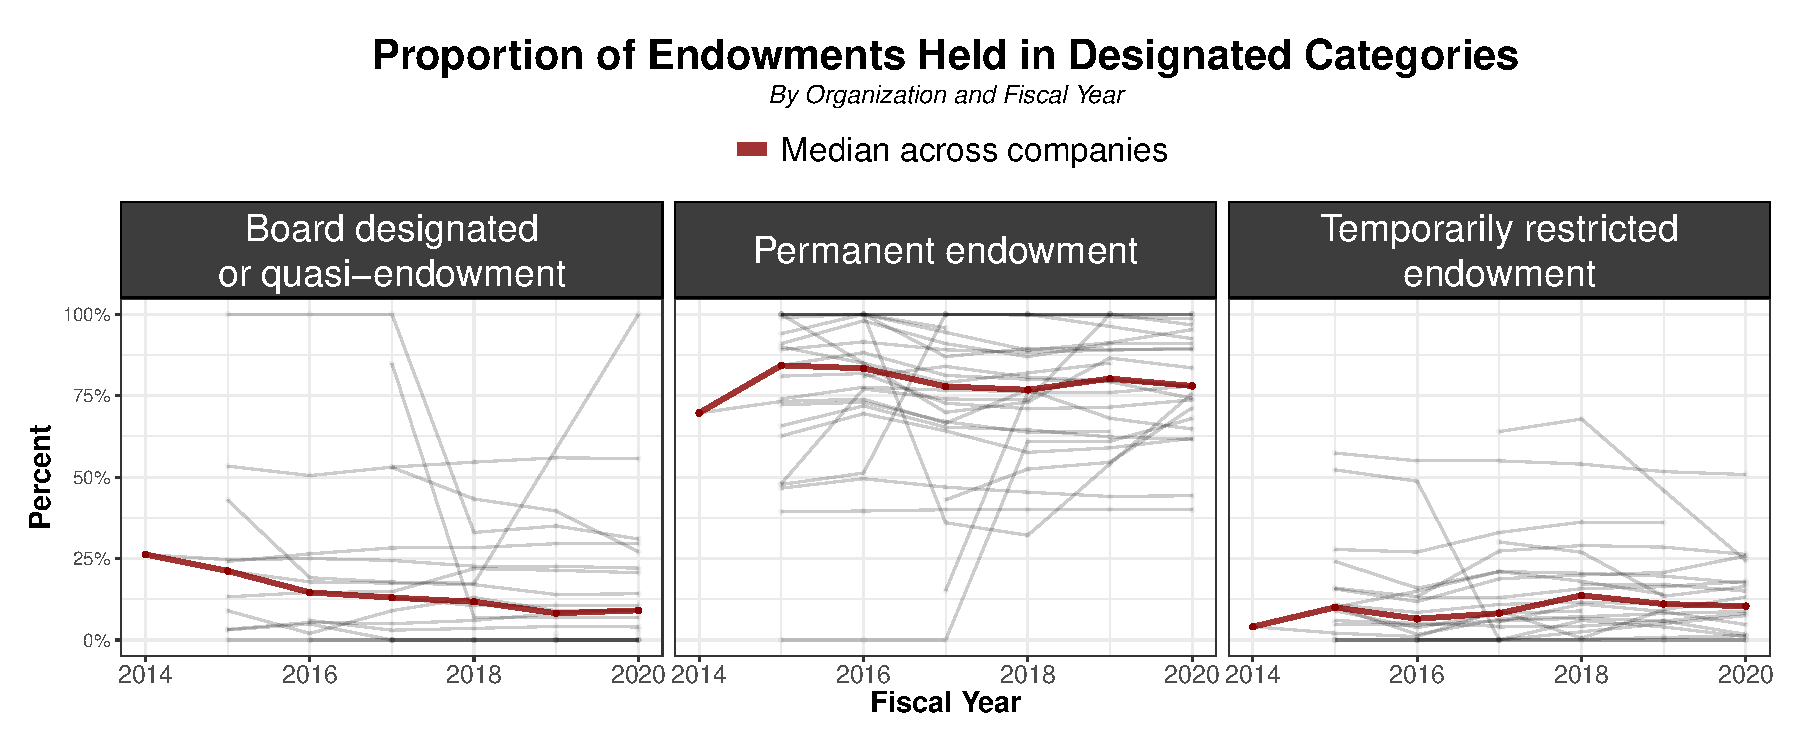
\includegraphics[width=0.9\linewidth,]{../images/proportion_endowment_categories} \caption{\label{fig:endowment-type}The percent of endowments held as a temporarily restricted endowment, permanent endowment, or board designated or quasi-endowment. The median across all companies by fiscal year is shown in red.}\label{fig:proportion-endowment-categories}
\end{figure}

However, there are several notable exceptions to the general trend of
consistency across years. Defining variability as the maximum standard
deviation of the proportions for each category, the most variable 5
companies were Fort Wayne Ballet, San Francisco Ballet, Nashville
Ballet, Atlanta Ballet, and the Washington Ballet (Figure
\ref{fig:prop-most-variable}).

\begin{itemize}
\item For Fort Wayne Ballet, most of the endowment funds (86\%) were board designated/quasi-endowment in 2017, but this dropped to a mere 7\% in 2018. The percentage of the endowment funds in the permanent endowment category increased accordingly. 
\item 100\% of San Francisco Ballet’s endowment was in the board designated/quasi-endowment category up until 2018, when the percentage in  board designated/quasi-endowment  dropped to 33\% and most (61\%) was a permanent endowment.
\item  The trends in Nashville Ballet’s endowment went the opposite direction, with a large increase in the percentage in the  board designated/quasi-endowment  category (17\% to 74\%) and decrease in the percentage in the permanent category.
\item For Atlanta Ballet, there is a dramatic shift in 2017 where the percentage held as temporarily restricted goes from 0\% to 64\%.
\item The Washington Ballet had a high proportion of its endowment in the temporarily restricted category (52\%) but by 2017 all their endowment funds were in the permanent endowment category. 
\end{itemize}

\begin{figure}[H]
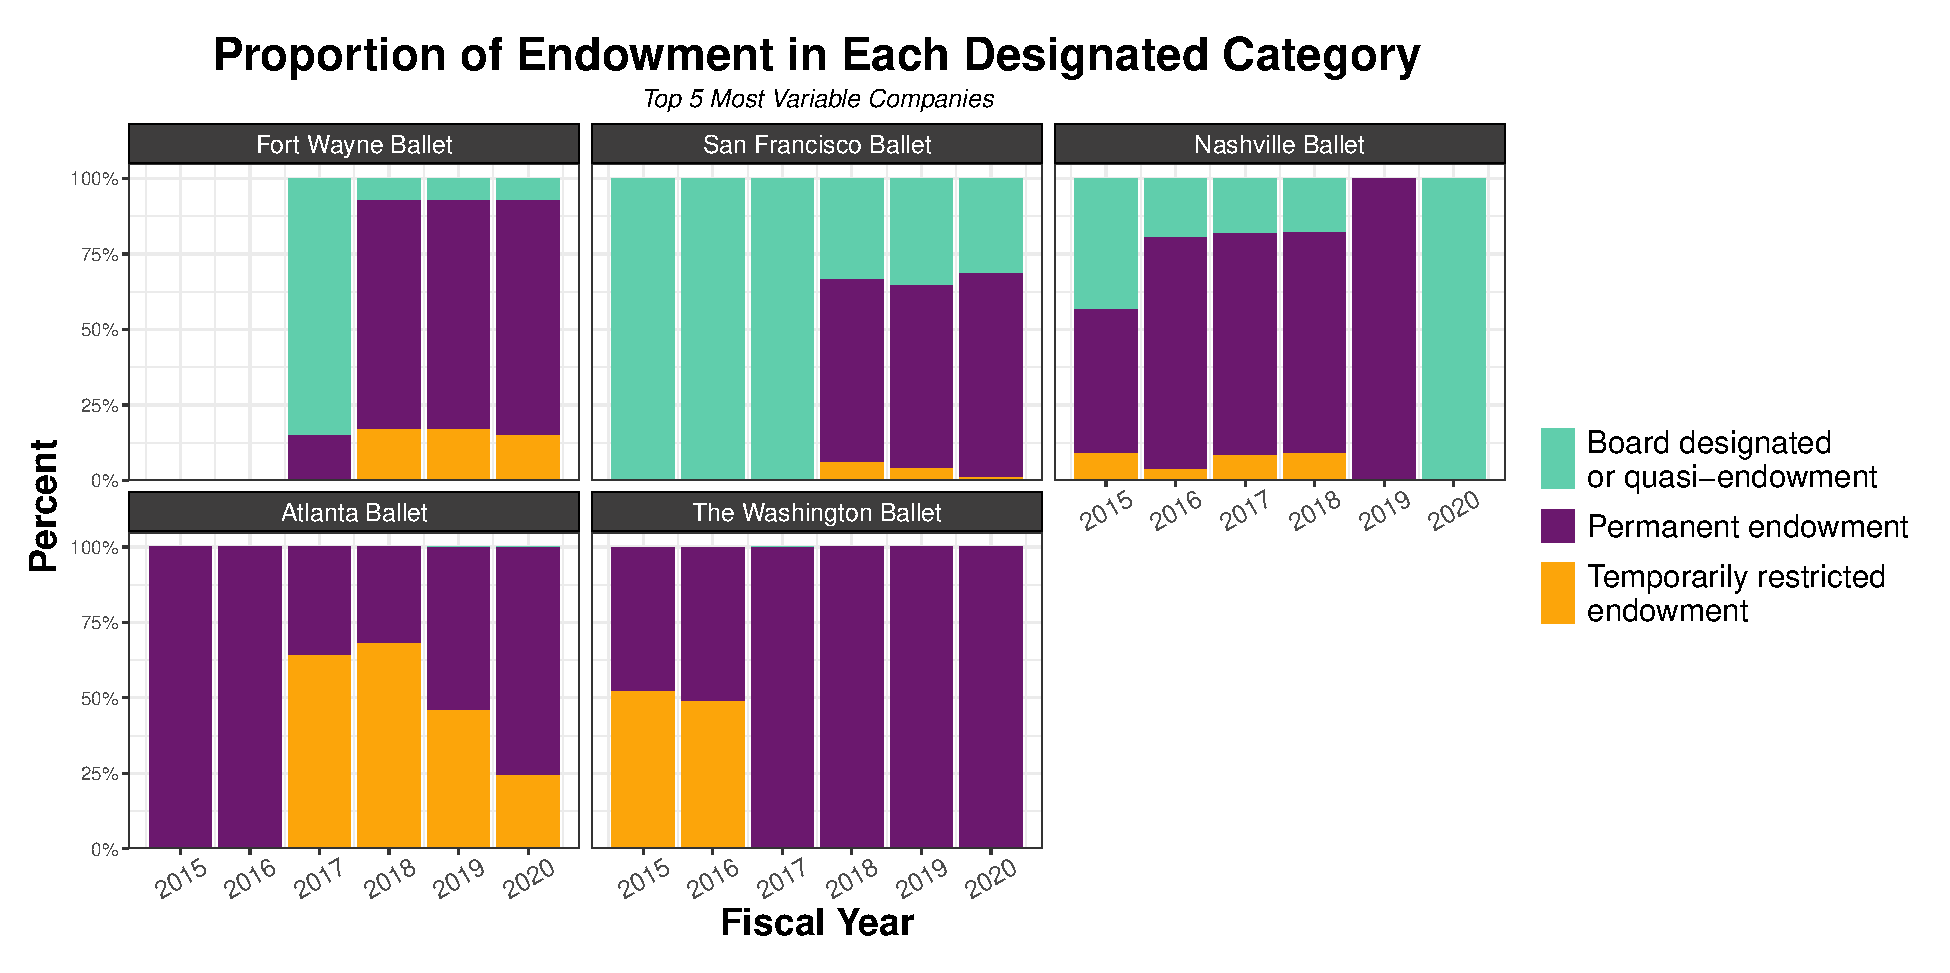
\includegraphics[width=0.9\linewidth,]{../images/prop_endowment_type_most_variable} \caption{\label{fig:prop-most-variable} Proportions of endowments in each designated category over time for the 5 companies with the most variability. We defined the most variable companies by considering the maximum standard deviation in the proportion in any one category.}\label{fig:proportion-endowment-categories-most-variable}
\end{figure}

\hypertarget{which-companies-have-endowments}{%
\subsubsection{Which Companies Have
Endowments?}\label{which-companies-have-endowments}}

As we discuss these endowment analyses, one of the most fundamental
questions about endowments is how many companies report them, and how
that varies over time. To report endowments, nonprofits fill out
Schedule D in Form 990. Out of 169 dance companies we investigated, 47
reported endowments at least once in Schedule D (Table
\ref{table:filled-scheduled}).

\begin{table}[!h]

\caption{\label{tab:unnamed-chunk-2}\label{table:filled-scheduled}Number of Companies that Reported an Endowment}
\centering
\begin{tabular}[t]{>{\raggedright\arraybackslash}p{10em}>{\raggedleft\arraybackslash}p{10em}>{\raggedleft\arraybackslash}p{10em}}
\toprule
 & Reported an Endowment & Did Not Report an Endowment\\
\midrule
\addlinespace[0.5em]
\multicolumn{3}{l}{\textbf{By Year}}\\
\hline
\hspace{1em}2014 & 6 & 1\\
\hspace{1em}2015 & 70 & 35\\
\hspace{1em}2016 & 79 & 37\\
\hspace{1em}2017 & 83 & 42\\
\hspace{1em}2018 & 96 & 40\\
\hspace{1em}2019 & 106 & 40\\
\hspace{1em}2020 & 83 & 40\\
\hspace{1em}2021 & 21 & 6\\
\addlinespace[0.5em]
\multicolumn{3}{l}{\textbf{\makecell[l]{Reported an Endowment\\at Least Once}}}\\
\hline
\hspace{1em} & 122 & 47\\
\bottomrule
\end{tabular}
\end{table}

\hypertarget{consistency-of-endowment-reporting}{%
\subsubsection{Consistency of Endowment
Reporting}\label{consistency-of-endowment-reporting}}

In investigating frequency of reporting endowments, we can see that most
companies who report an endowment continue to consistently do so across
their 990 filings (Figure \ref{fig:gap-plot}). Some, however, including
Oregon Ballet Theater and Ballet Des Moines, begin reporting an
endowment well after their first filed 990. Other companies such as The
Charleston Ballet, Colorado Ballet, and American Repertory Ballet stop
reporting endowments.

\begin{figure}[H]
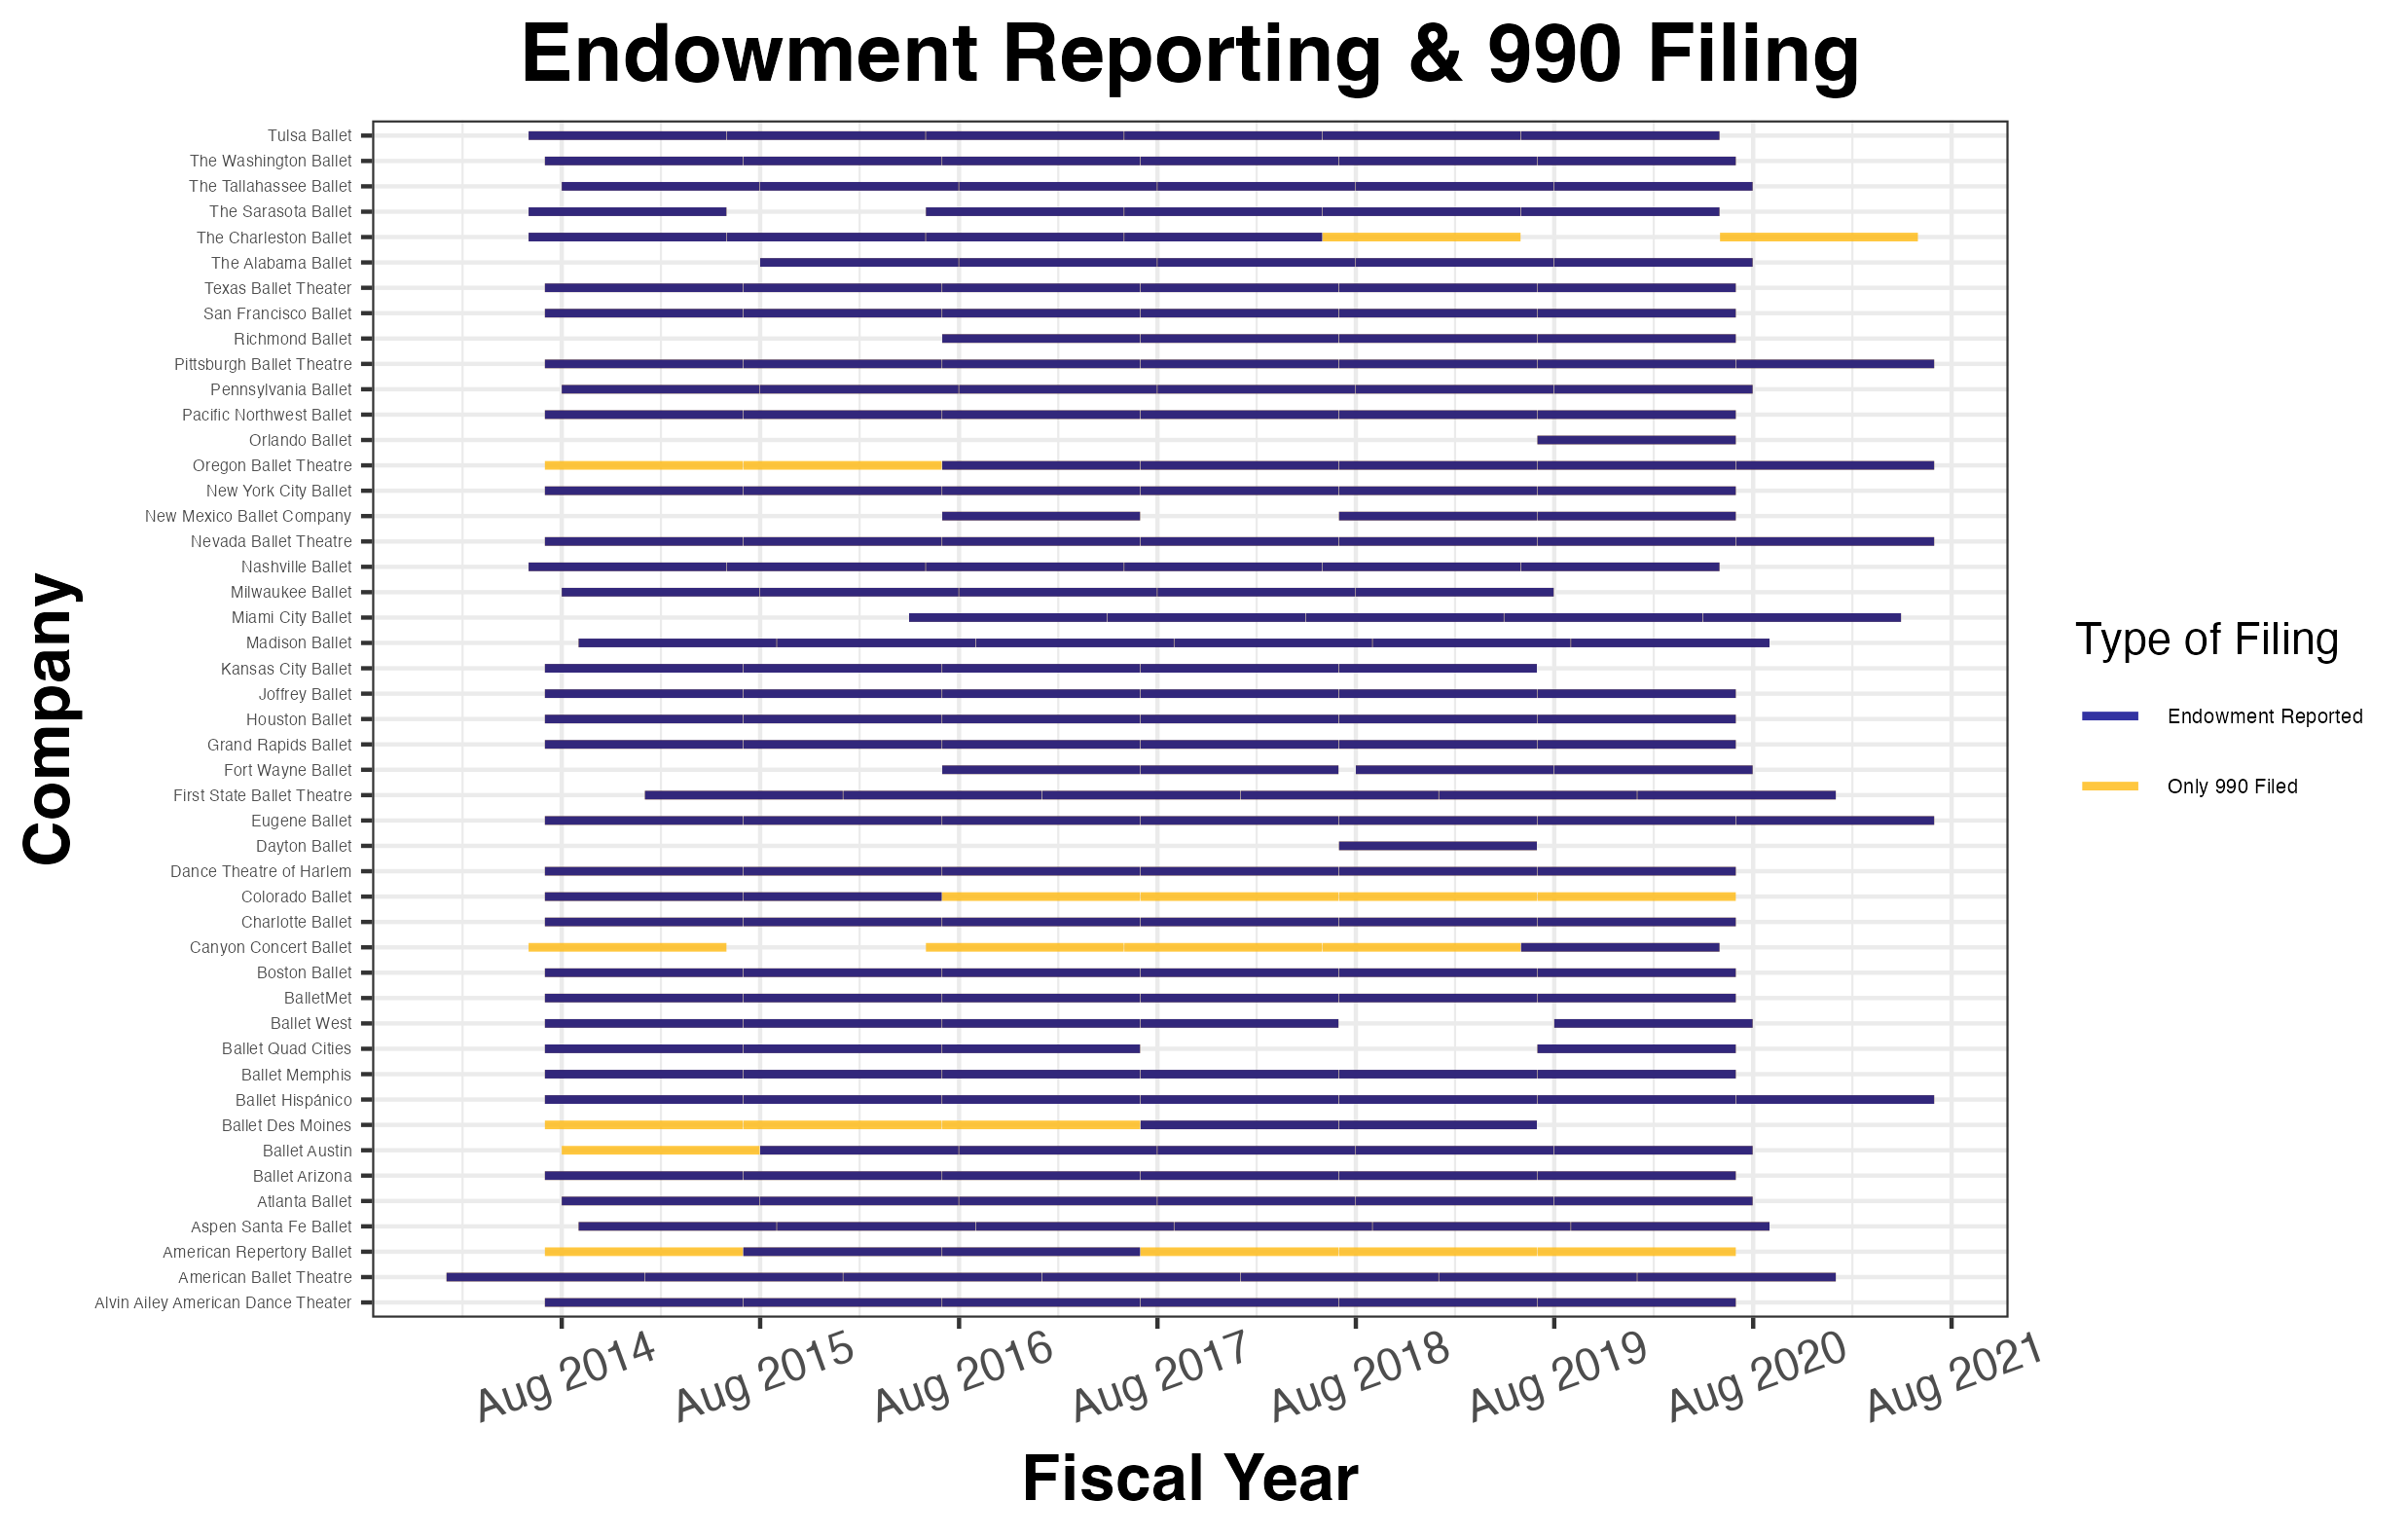
\includegraphics[width=0.9\linewidth,]{../images/gap_plot_endowment} \caption{\label{fig:gap-plot}Continuity of filings among dance companies; gaps in a companies' filings correspond to missing fiscal years.}\label{fig:unnamed-chunk-3}
\end{figure}

\hypertarget{ranking-companies-endowments}{%
\subsubsection{Ranking Companies'
Endowments}\label{ranking-companies-endowments}}

Ranking companies can be useful to see how endowments did relative to
each other rather than looking at the raw values, which are on immensely
different scales.

When we look at the rankings of the beginning of year balance of
companies' endowments, we see immediately that the top 7 companies, New
York City Ballet, San Francisco Ballet, Houston Ballet, Alvin Ailey
American Dance Theater, American Ballet Theatre, Pacific Northwest
Ballet, and Boston Ballet, see no changes in ranking from 2013 to 2020
(Figure \ref{fig:rank-endowments}) .

Below the top 7, there are more shifts in the rankings across time, with
some companies changing dramatically in ranking. This includes:

\begin{itemize}
\item A dramatic decrease in Aspen Santa Fe Ballet’s ranking from 2018 through 2020
\item A marked increase in: 
\subitem - Joffrey Ballet’s ranking
\subitem - Orlando Ballet’s ranking
\subitem - Fort Wayne Ballet’s ranking
\subitem - Ballet Arizona’s ranking
\item A decrease in Atlanta Ballet’s ranking from 2013 to 2015 that then recovered.
\end{itemize}

\begin{figure}[H]
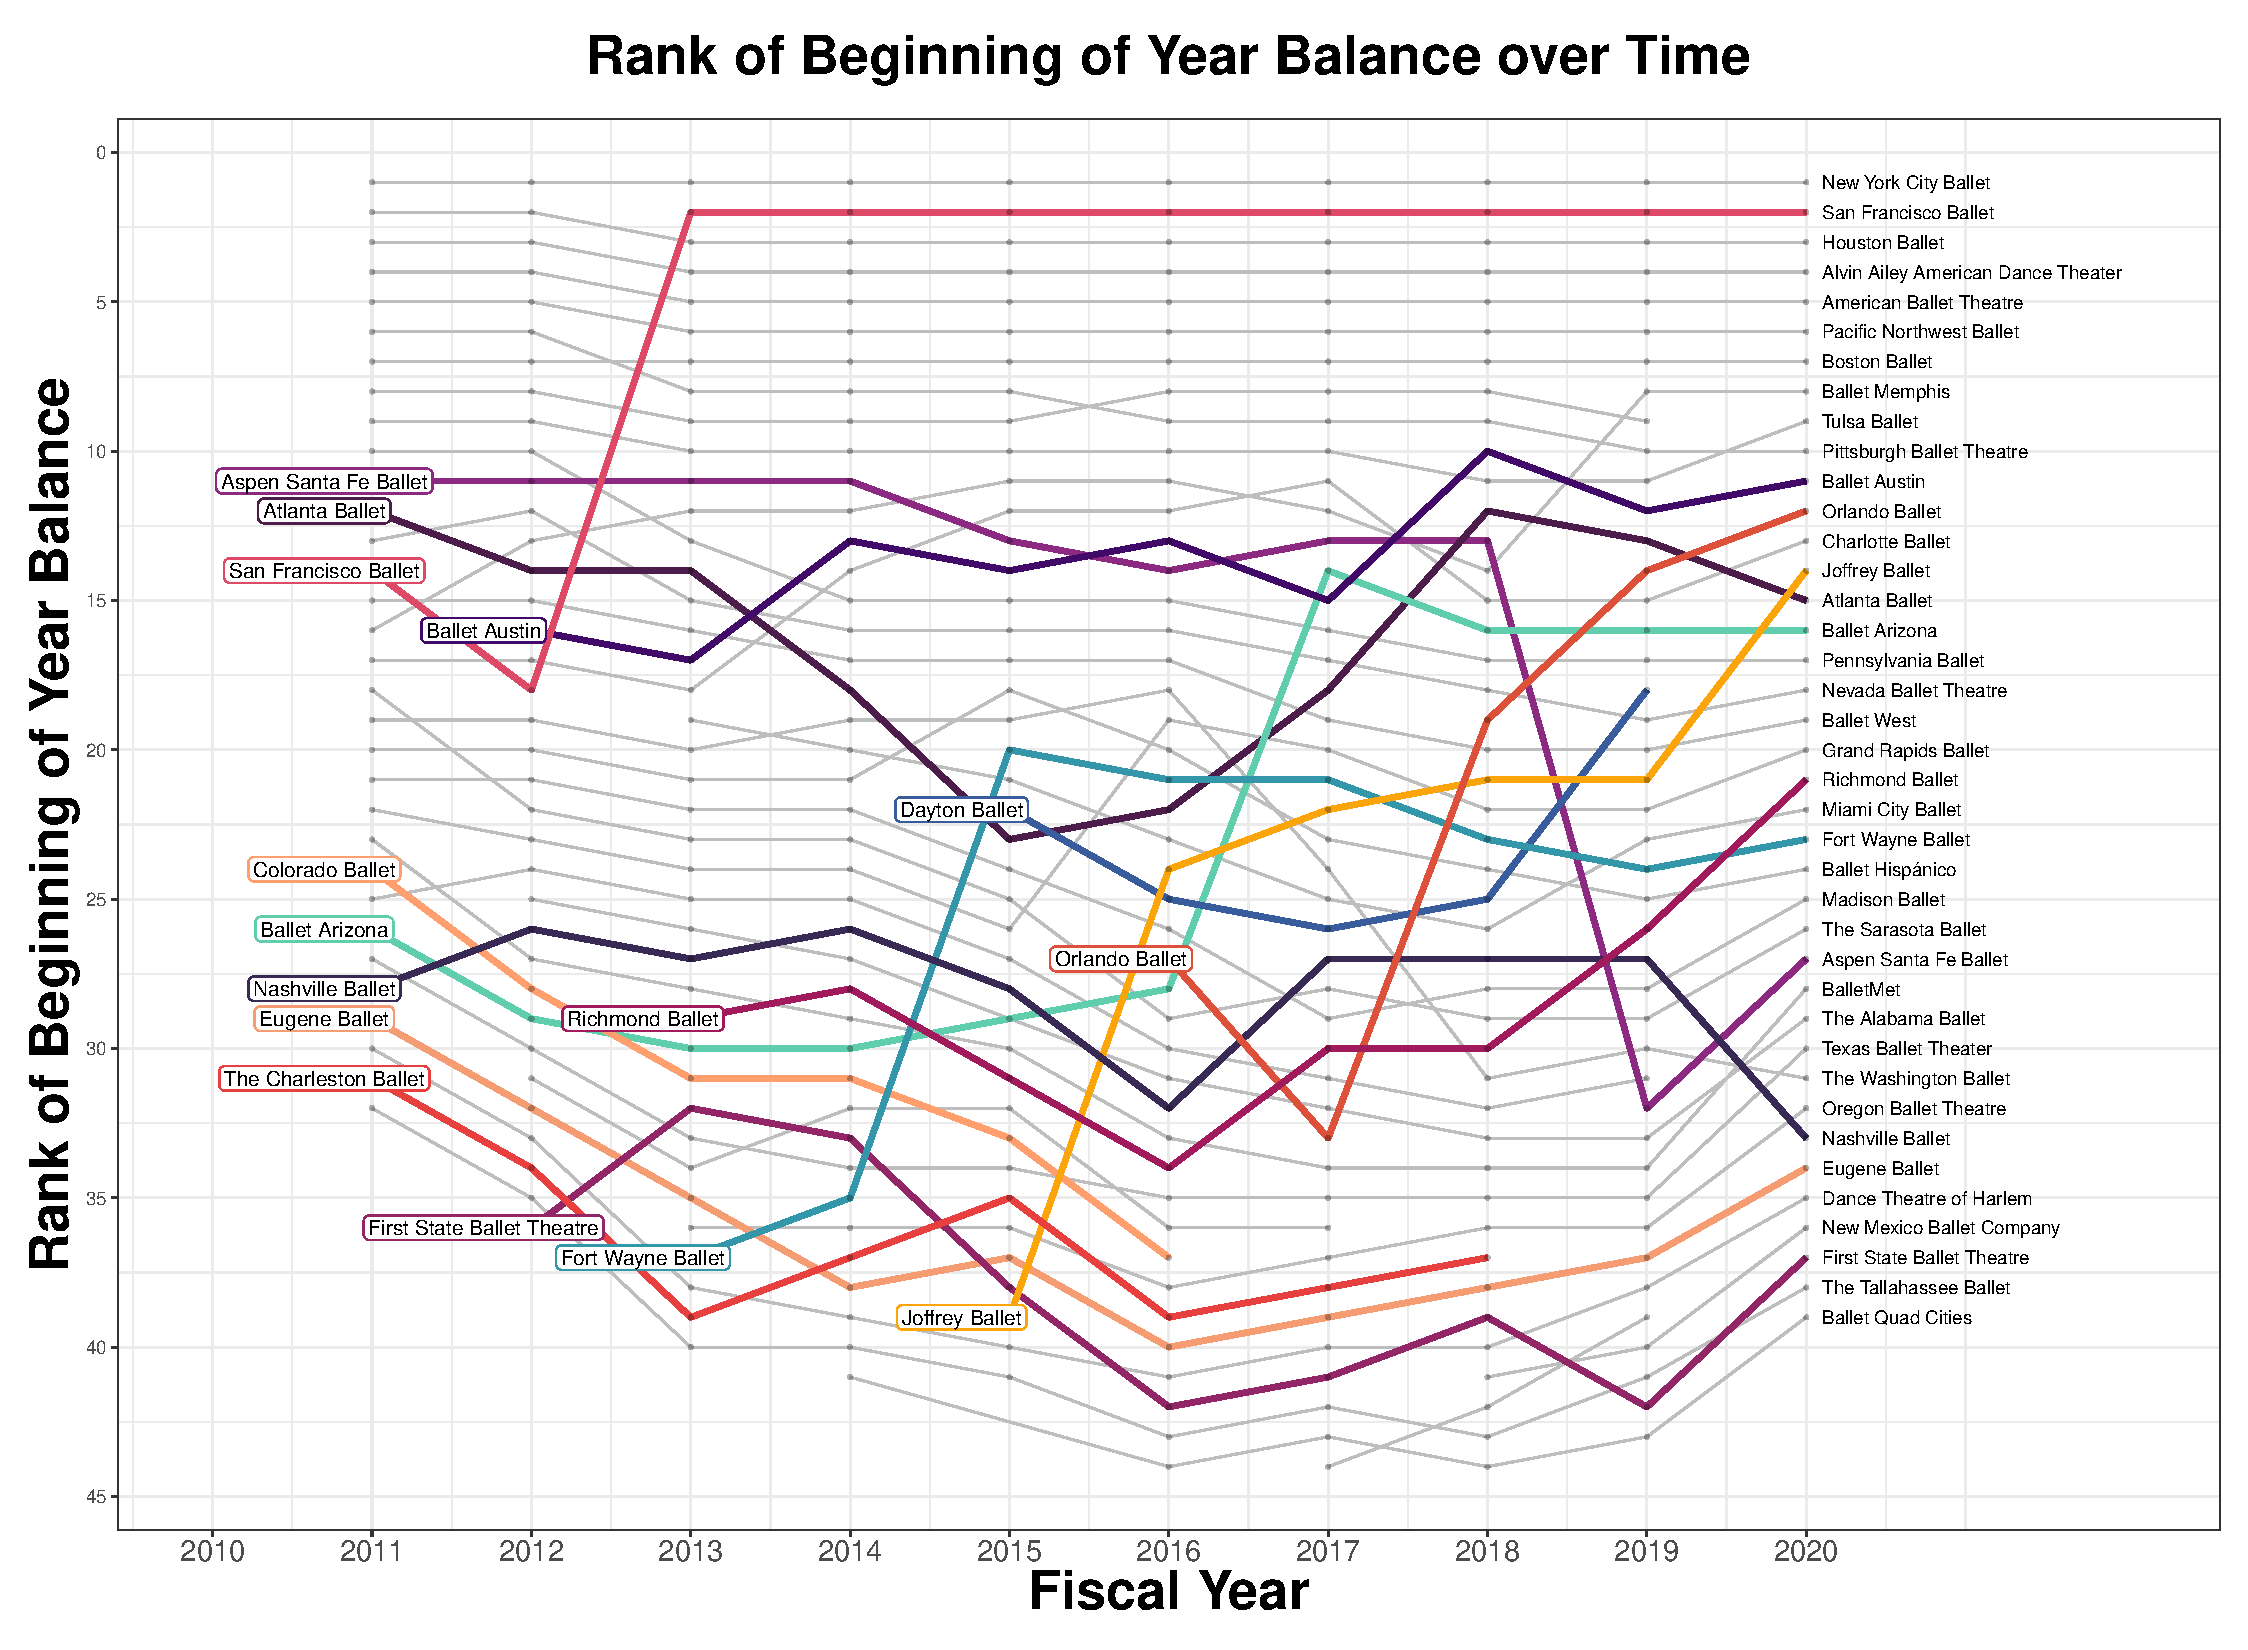
\includegraphics[width=0.9\linewidth,]{../images/rank_of_beginning_year_balance} \caption{\label{fig:rank-endowments}Rank of the endowment beginning of year balance over time. The 15 companies with the most variability in ranking, defined as the mean difference in rankings between fiscal years, are shown in color. Names of all companies are on the right.}\label{fig:rank-og-beginning-year-balance}
\end{figure}

When we add information on how these companies ranked in contributions
(Figure \ref{fig:rank-endowments-color-contribution}), we see that
although some organizations that are top ranked in endowment balance are
also top ranked in mean contributions, several of the companies that
experienced notable changes in their rankings also were ranked high in
contributions, in particular, Orlando Ballet and Joffrey Ballet.

\begin{figure}[H]
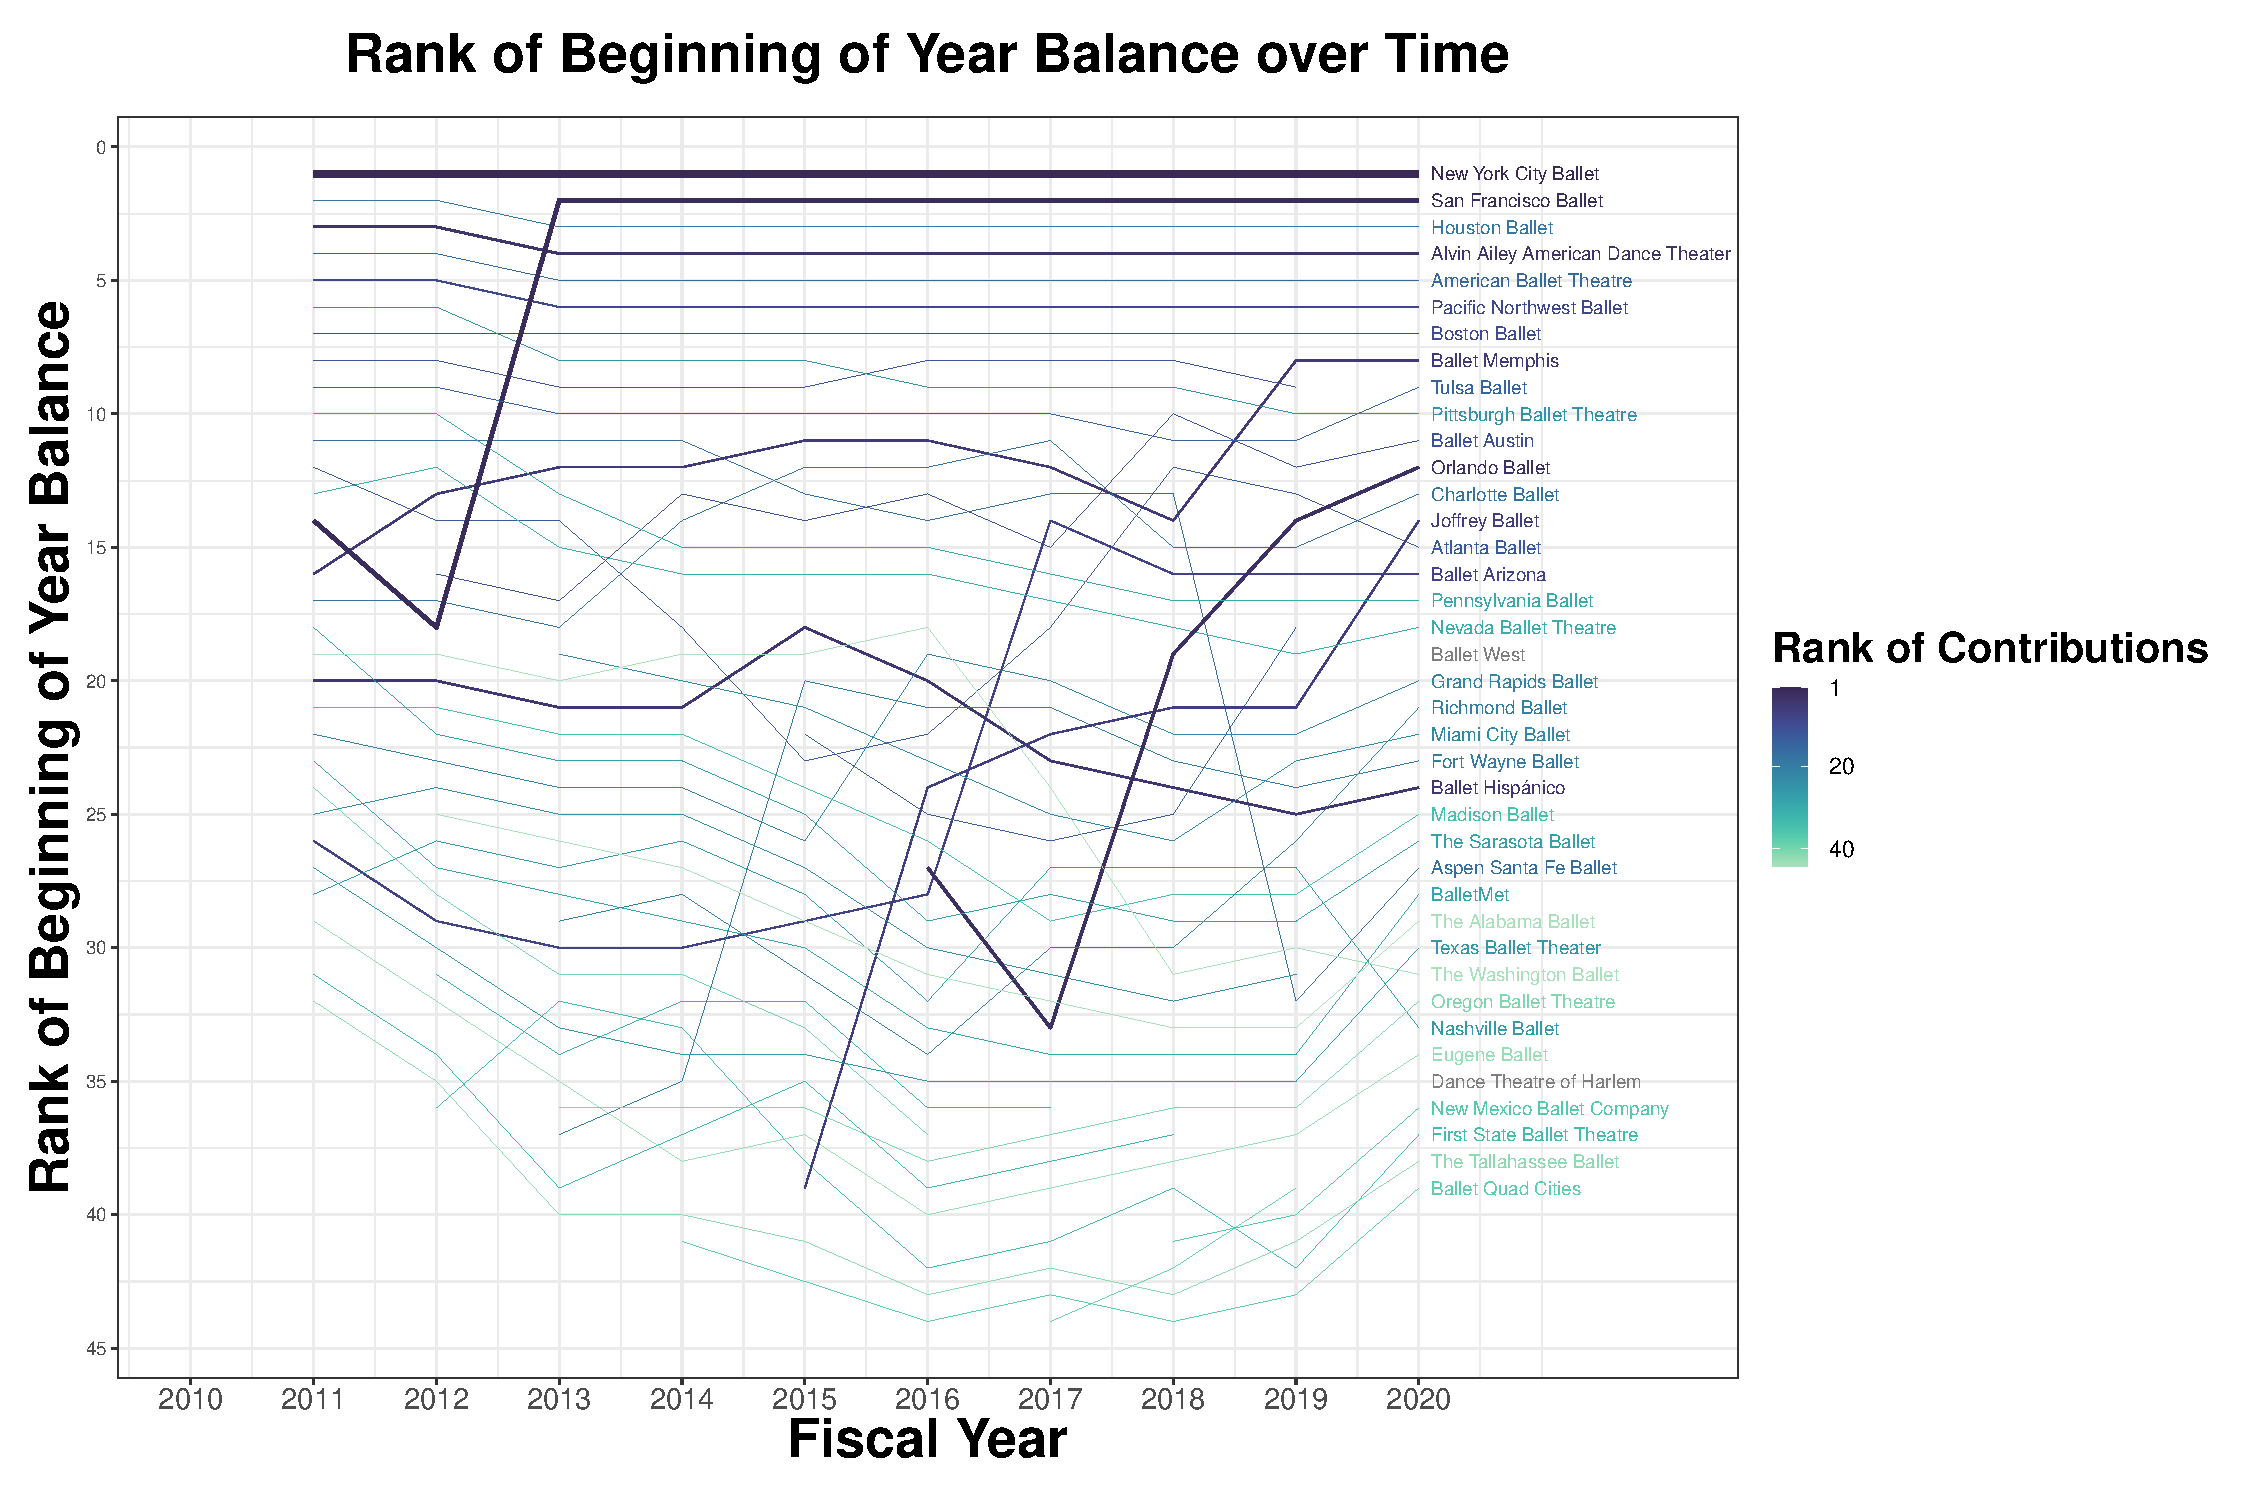
\includegraphics[width=0.9\linewidth,]{../images/rank-endowments-color-contribution} \caption{\label{fig:rank-endowments-color-contribution}Rank of the endowment beginning of year balance over time, where the color indicates the ranking of the mean contributions received over all years on file for the company.}\label{fig:unnamed-chunk-4}
\end{figure}

Looking more closely at the relationship between contribution rankings
and beginning of year balance rankings, in Figure \ref{fig:balancecont},
there is a strong relationship between how a company ranks with regard
to their contributions relative to the other companies and how a company
ranks in the endowment beginning of year balance. That is, when
companies are ranked high in the beginning of year balance, they tend to
rank high in contributions as well. As we would expect, this trend holds
across the full set of fiscal years considered.

However, the rankings are often not identical. If they were, all points
would fall on the red line, which represents an exact correspondence
between rankings. In some cases, a company consistently ranks higher in
contributions relative to the beginning of year balance. We summarize
whether the contributions or beginning of year balance tends to rank
higher for a given company in Figure \ref{fig:balancecontbar}. For
example, Ballet West ranked higher in the endowment beginning of year
balance for each year available (2016-2020), while Nashville Ballet
ranked higher in contributions than beginning of year balance for every
year on file (2011 - 2022).

\begin{figure}[H]
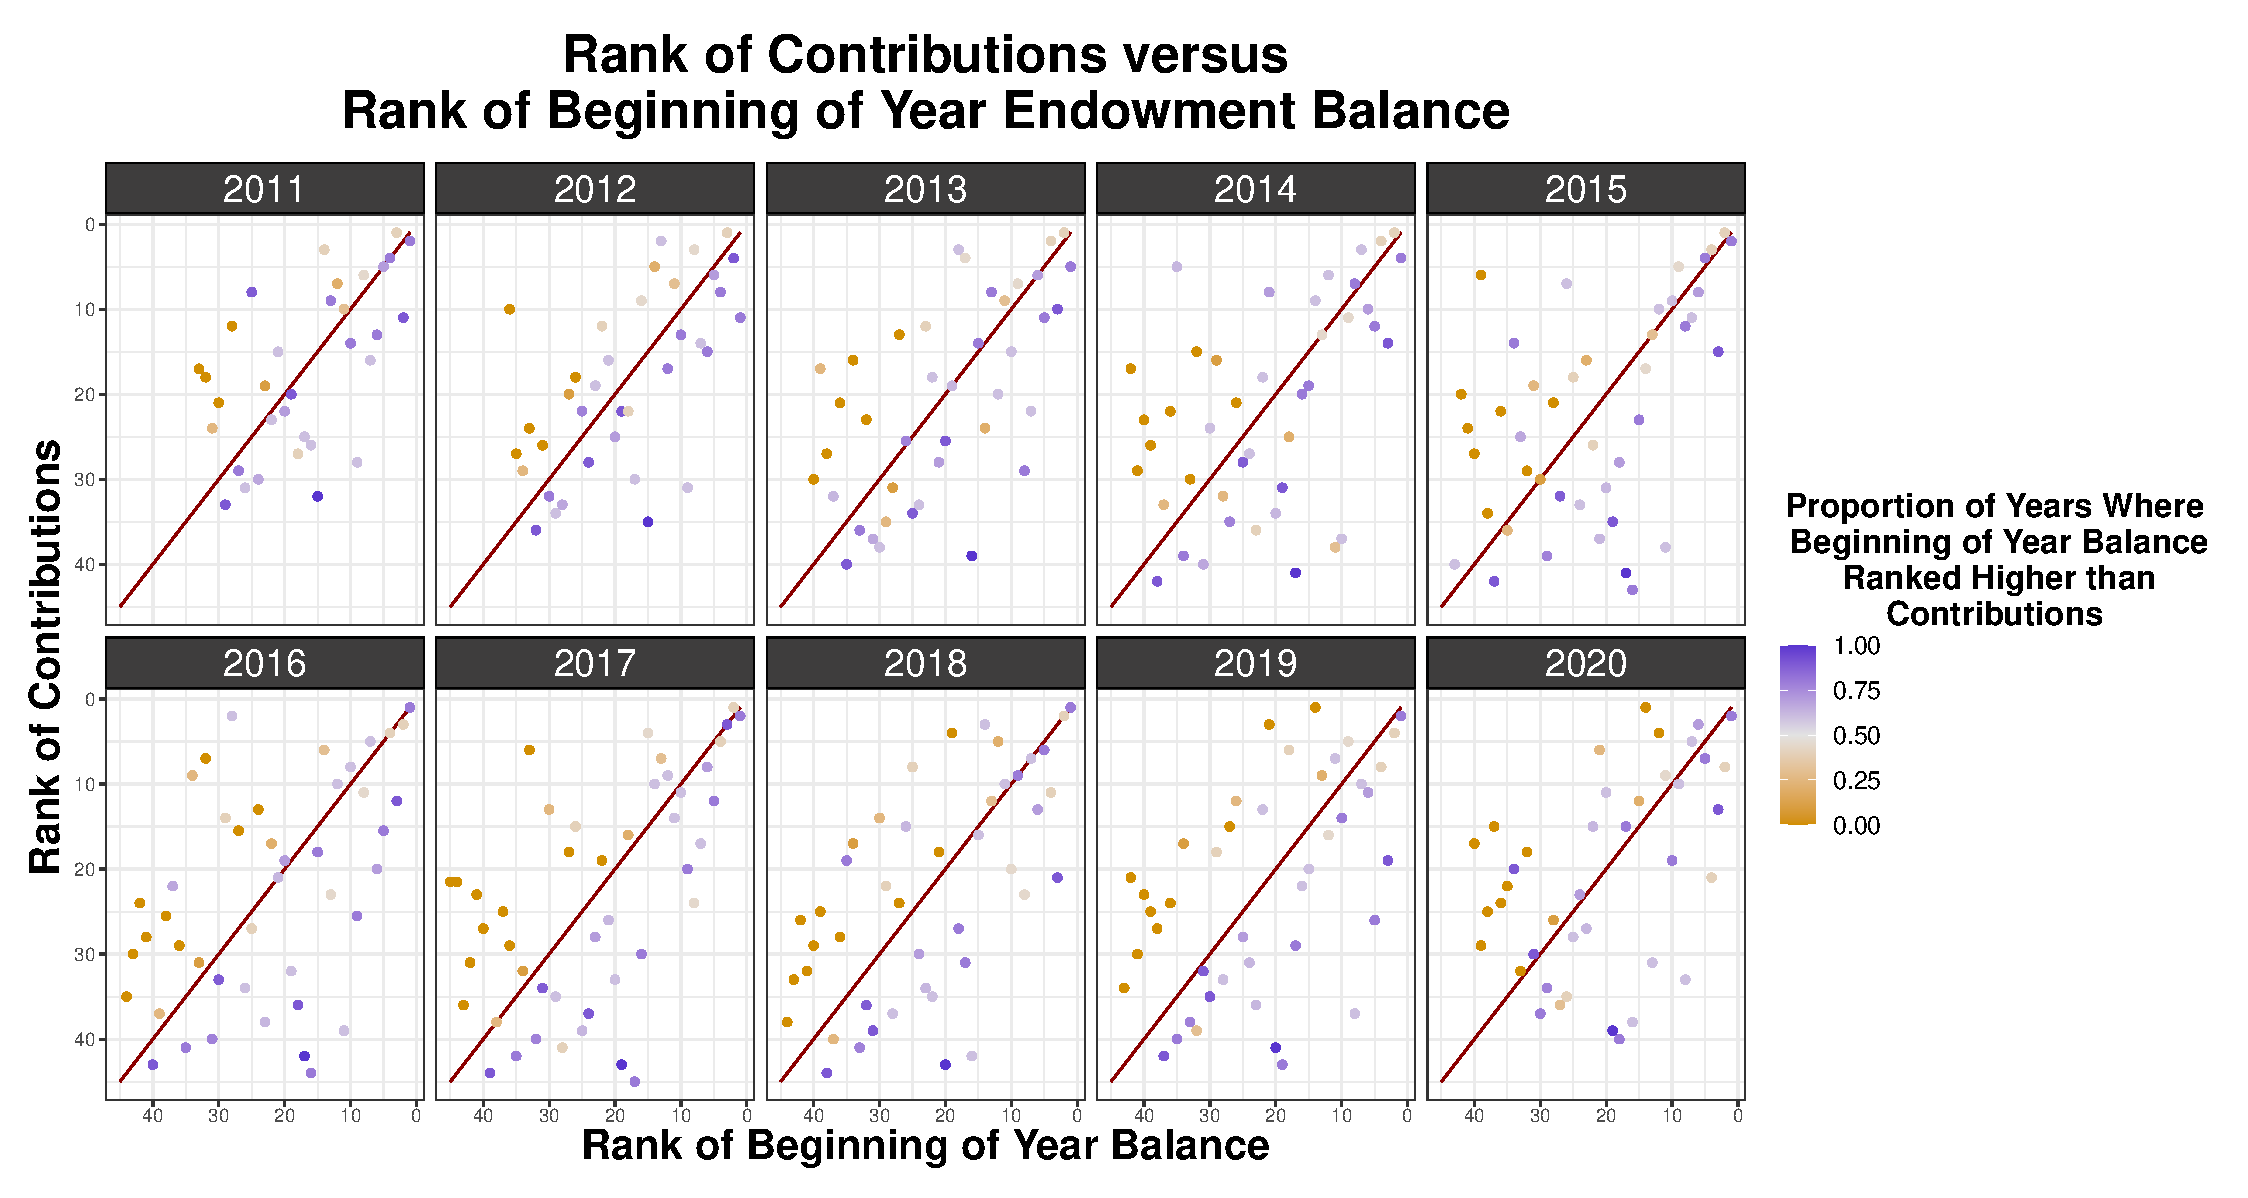
\includegraphics[width=0.75\linewidth,]{../images/compare-rankings-balance-contributions} \caption{\label{fig:balancecont} Comparing the rankings of beginning of year balance of the endowment to the ranking of contributions recieved.}\label{fig:compare-rankings-balance-contributions}
\end{figure}

\begin{figure}[H]
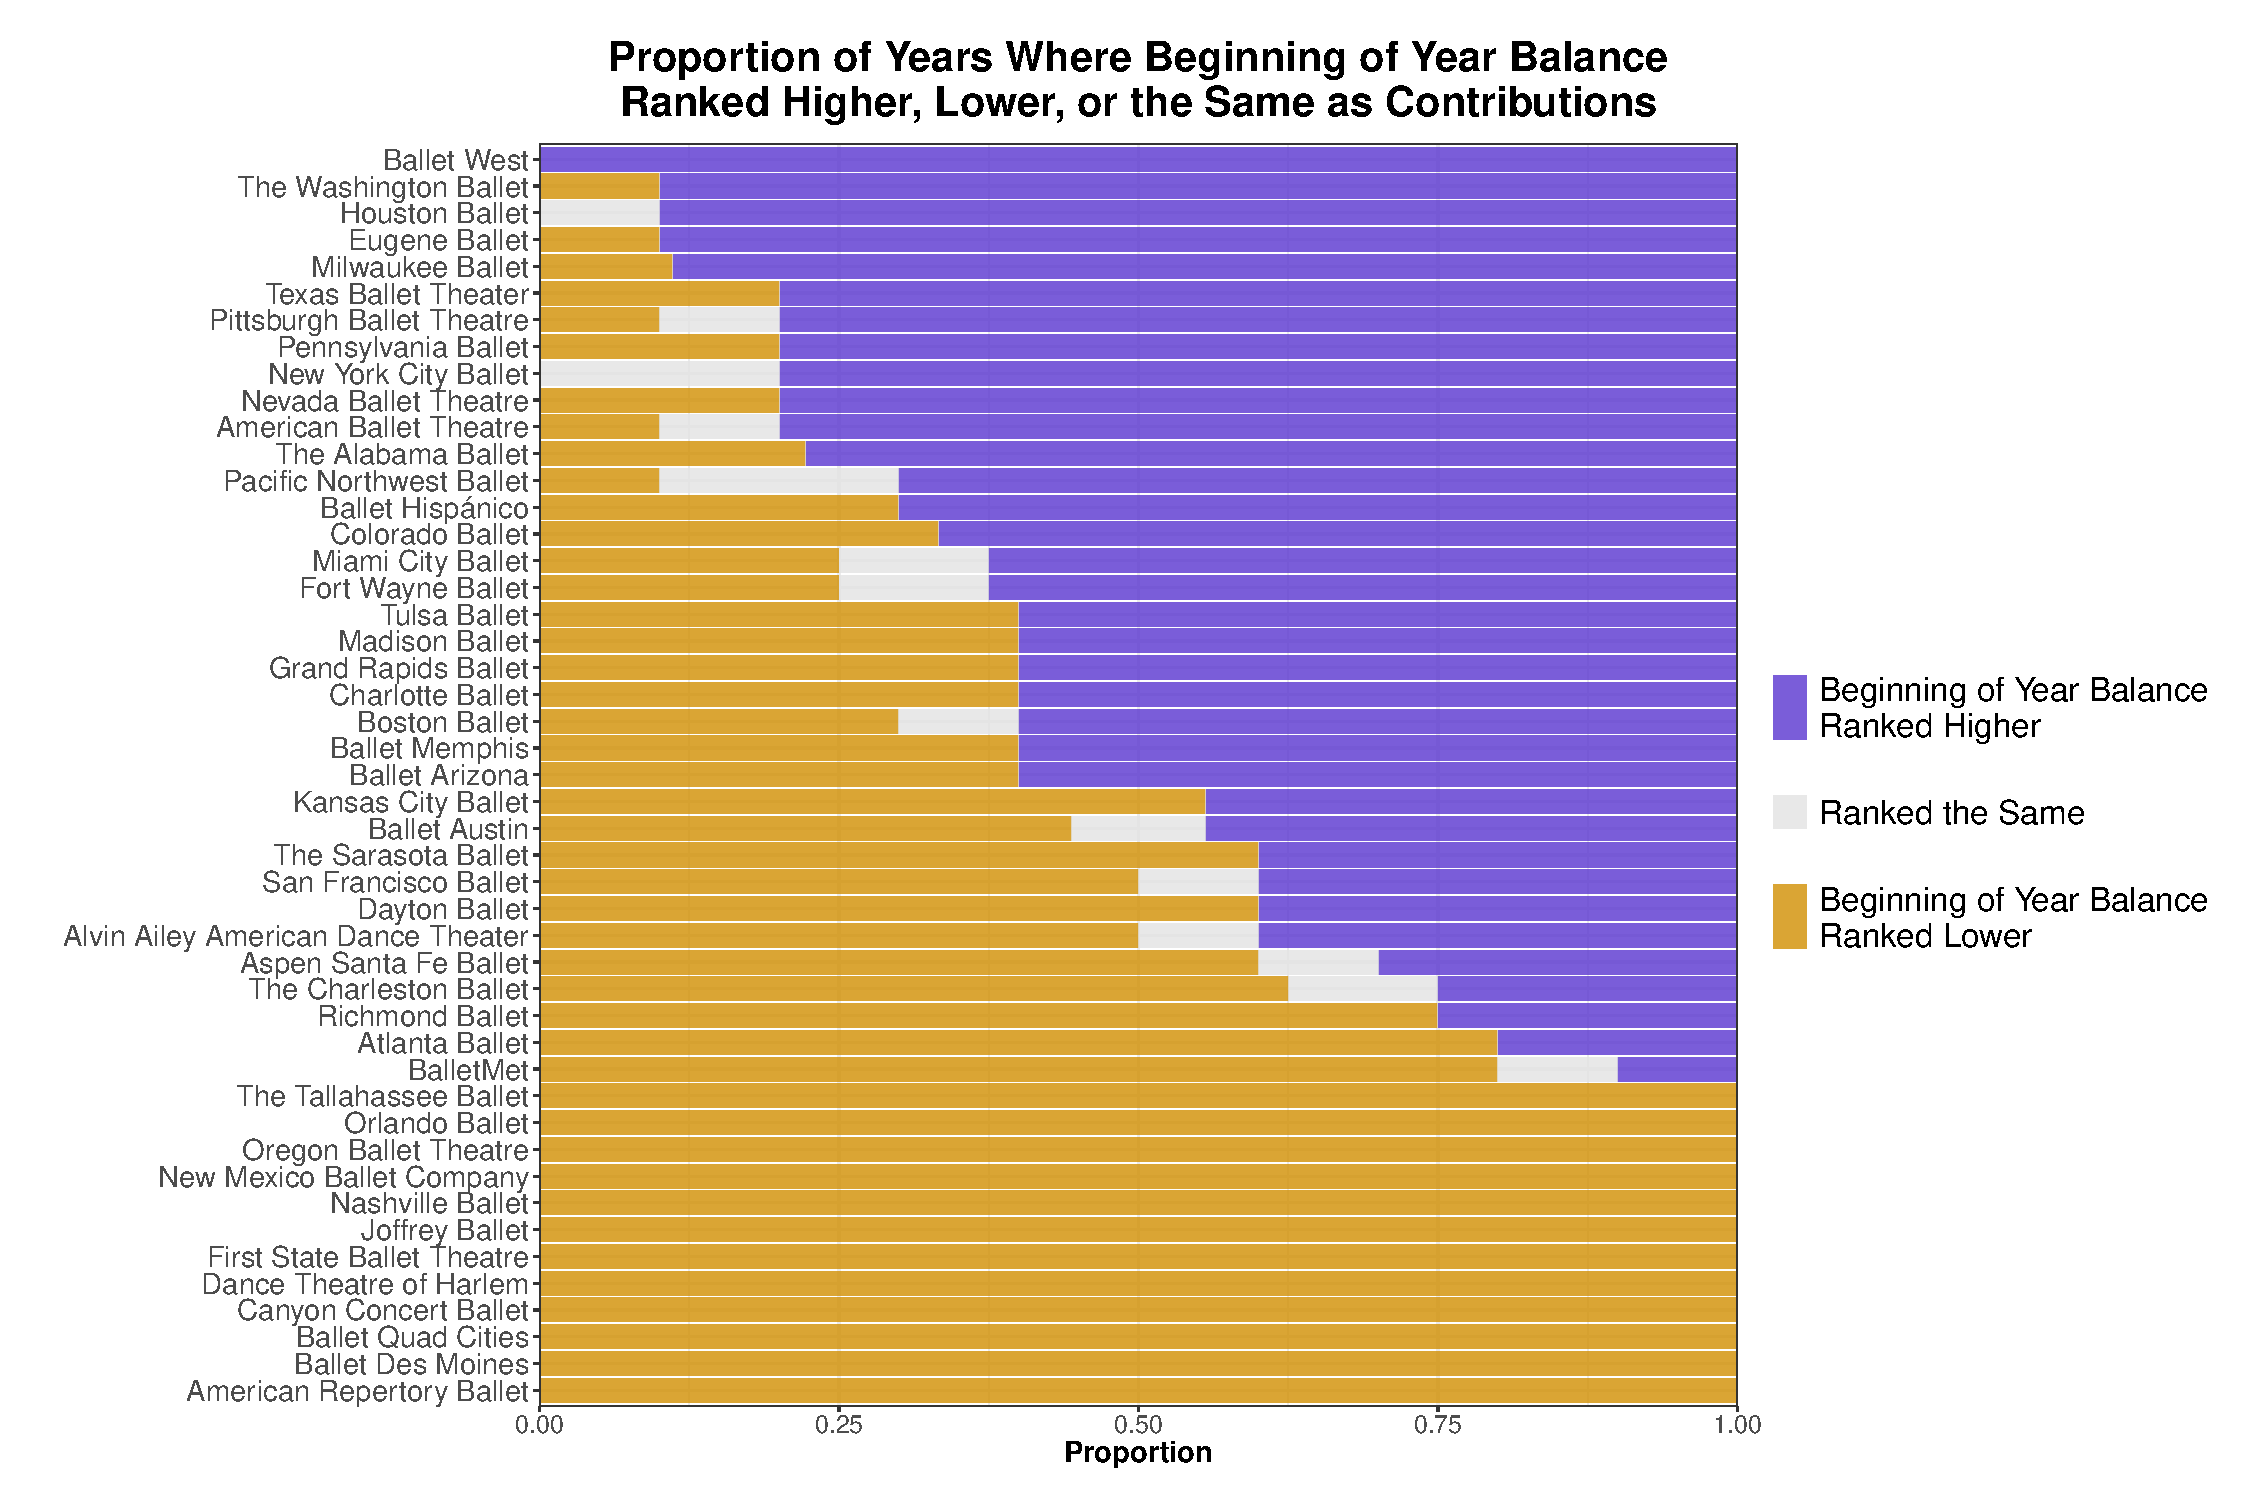
\includegraphics[width=0.75\linewidth,]{../images/compare-rankings-balance-contributions-barplot} \caption{\label{fig:balancecontbar} Comparing the proportion of years where a company ranked higher, lower, or the same in beginning of year balance compared to contributions received. A higher rank means a rank closer to 1, where 1 is the top possible rank.}\label{fig:compare-rankings-balance-contributions-barplot}
\end{figure}

In contrast to what we saw in the rankings of the beginning of year
balance (Figures \ref{fig:rank-endowments-color-contribution} and
\ref{fig:rank-endowments}, we see in Figure
\ref{fig:rankings-contributions} that the rankings of contributions are
much less consistent.

\begin{figure}[H]
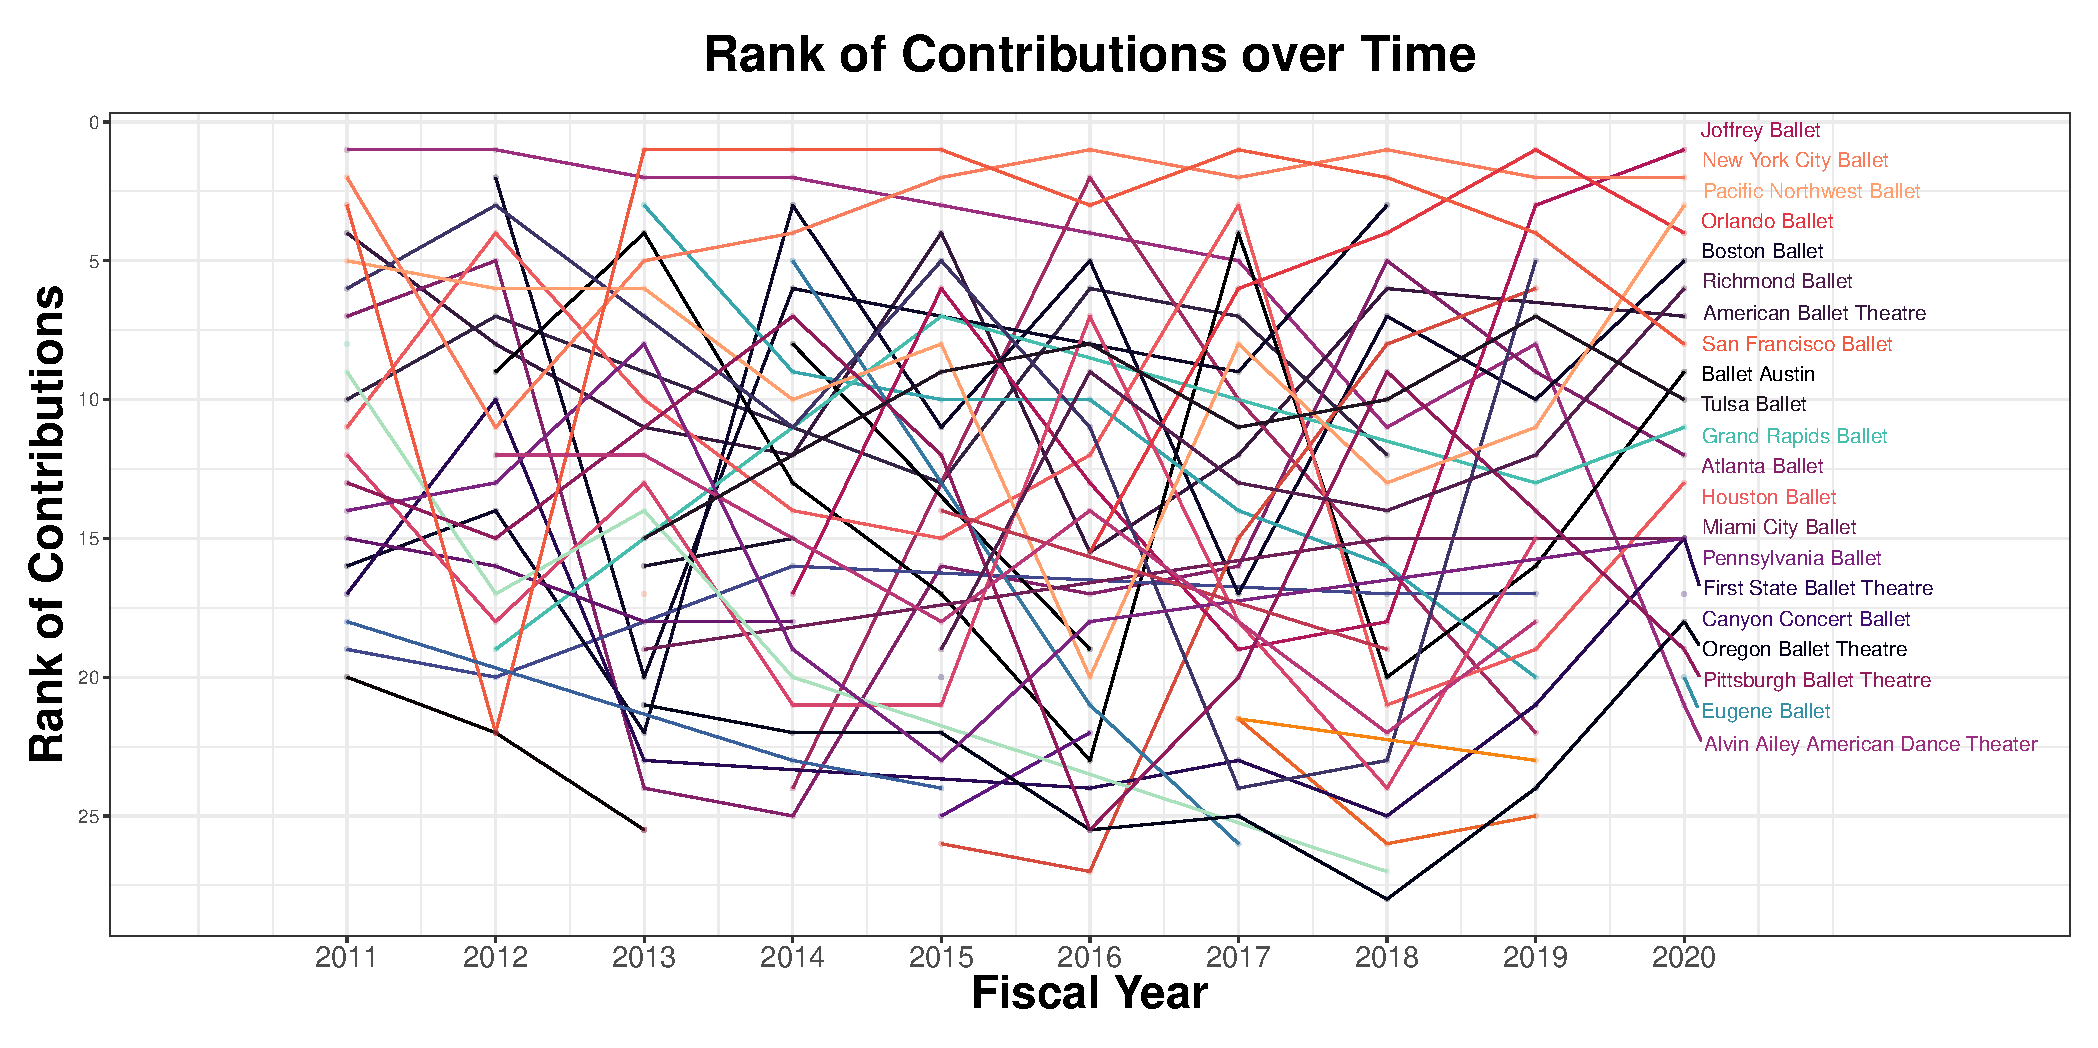
\includegraphics[width=0.9\linewidth,]{../images/ranking-contributions} \caption{\label{fig:rankings-contributions}The rankings of contributions over time, by organization.}\label{fig:ranking-contributions}
\end{figure}

\hypertarget{reported-endowment-balances-over-time---is-the-math-right}{%
\subsubsection{Reported Endowment Balances over time - Is the Math
right?}\label{reported-endowment-balances-over-time---is-the-math-right}}

\begin{quote}
Due to time constraints within our project, we did not have the
opportunity to reach out to any companies regarding their
miscalculations or negative expense reports. We hope to do this in the
future, prior to this report being published.
\end{quote}

Theoretically, one can calculate an endowment's fiscal year end balance
based on all information provided in Schedule D. We calculated the end
of year balance (see the equation below), and then compared our
calculated balance to the reported end of year balance. The majority of
calculations are concordant; however, we noted discrepancies in thirteen
companies. Discrepancies range from \$-20,000 (Orlando Ballet, 2016) to
\$8,301,066 (Atlanta Ballet, 2017). Due to the scaling of the below
figure, differences in reported and calculated balance below a hundred
thousand dollars are difficult to see.

\[\text{Calculated Year End Balance} = \text{Beginning Year Balance} + \text{Contributions} +\]
\[ \text{Investment Earnings or Losses} - |\text{Administrative Expenditures}| -\]
\[|\text{Other Expenditures}| - | \text{Grants or Scholarships}| \tag{1}\]

For values related to expenses (administrative expenditures, other
expenditures, grants or scholarships), we took the absolute value to
ensure all were positive numbers. Four companies (Ballet Hispánico,
Atlanta Ballet, Miami City Ballet, and Dance Theatre of Harlem) report
their other expenditures as a negative value; thus, when calculating end
year balance, subtracting a negative value would result in an additive,
not subtractive, effect.

We see the difference in the extent of discrepancies when we take the
absolute value (Figure \ref{fig:miscalc} (a)), as in equation (1),
versus when we do not (Figure \ref{fig:miscalc} (b)). There are less
discrepancies when we do take the absolute value.

Since we compute the difference by taking
\(\text{Reported End Balance} - \text{Calculated End Balance}\),
negative values indicate the calculated end balance was larger than the
reported, and positive values indicate the reported end balance was
larger. The calculated differences are split between being negative or
positive.

Atlanta Ballet has the largest discrepancy in (a); however, we see that
if we don't take the absolute value and take the negatives as is (b),
the values are concordant. The opposite issue occurs for Miami City
Ballet, whereby in (a) with the absolute value, they are concordant.
However, in (b) without absolute value of expenses, they appear eight
times. Both of these situations stem from reports of negative values in
an expenses column, although they are mirrored situations. Thus, this
raises the question as to how negative expenses should be dealt with.

Considering panel (a), most companies only miscalculate once; however,
there are multiple miscalculations for Fort Wayne Ballet, Atlanta
Ballet, and Ballet Arizona. Of note, some of these differences were
trivial (e.g., \$10). Eugene Ballet does not report an end year balance
for 2011, yet reports a beginning balance of \$45,000, hence the
-\$45,000 difference we see for this year.

\begin{figure}[H]
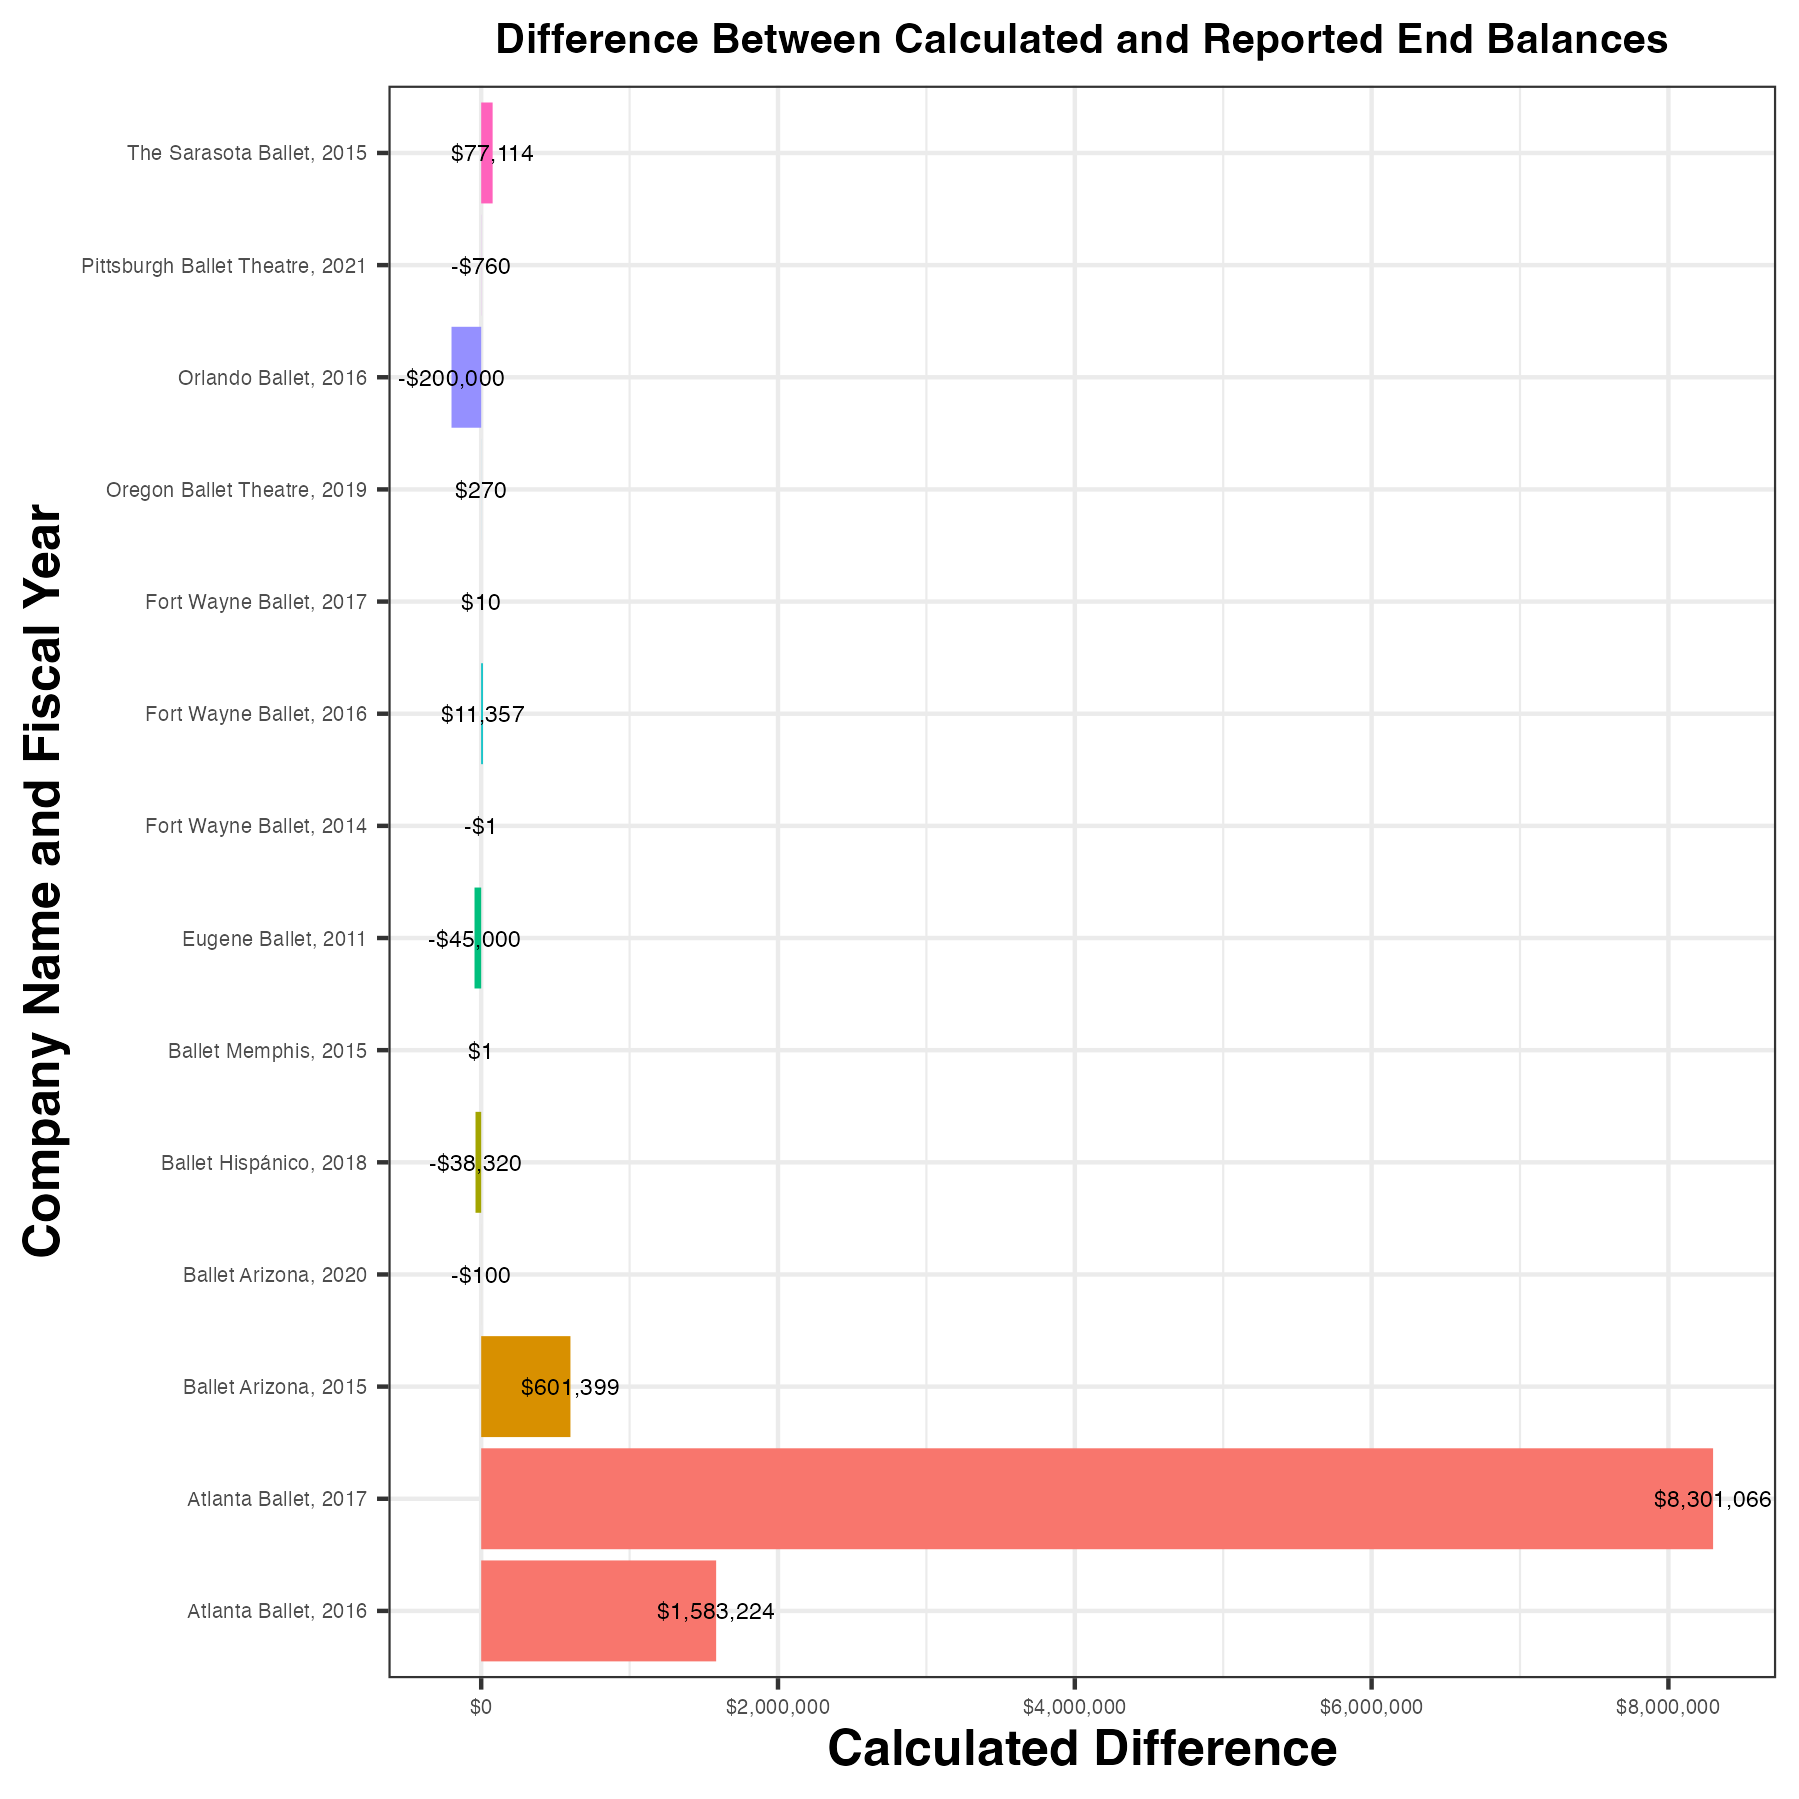
\includegraphics[width=0.5\linewidth,]{../images/diff_end_bal} 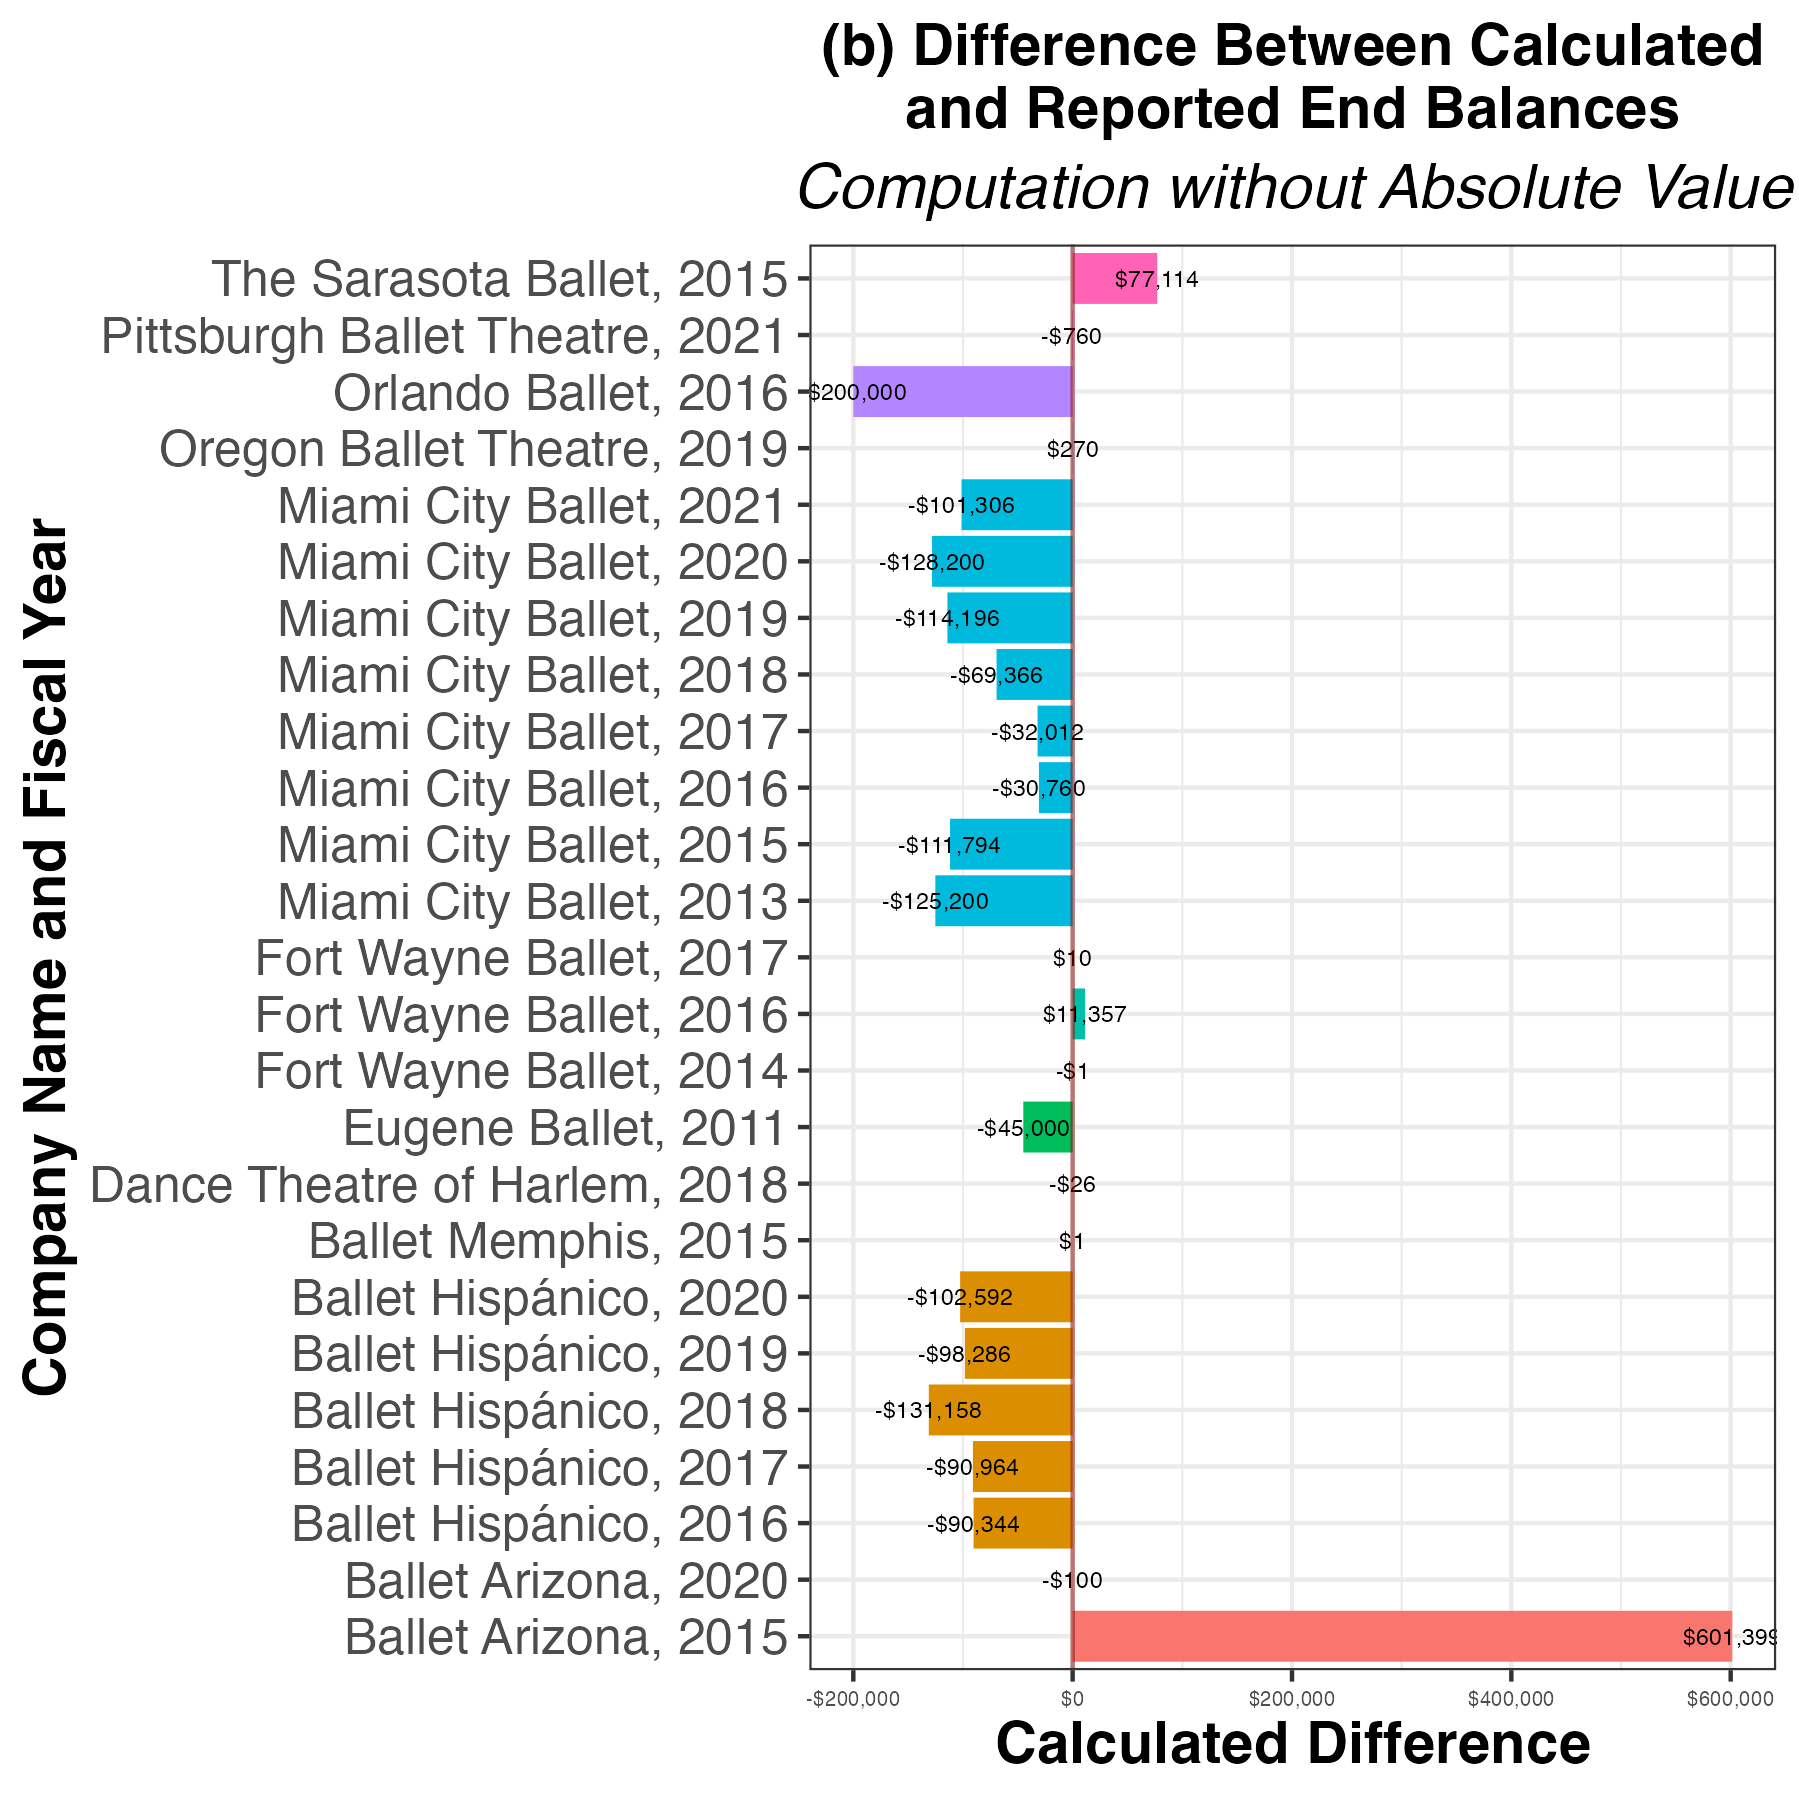
\includegraphics[width=0.5\linewidth,]{../images/diff_end_bal_no_abs} \caption{\label{fig:miscalc}Comparing the reported end of year balance to that we computed based on other reported variables. Calculation is done with the absolute value in (a) and without in (b). Each organization is in a different color.}\label{fig:unnamed-chunk-5}
\end{figure}

We summarize the discrepancies found by taking the absolute value
(e.g.~panel (a) of the above figure) in Figure
\ref{fig:miscalc-by-comp}. When taking the absolute value, the company
who misreports the most is Fort Wayne Ballet with three miscalculations.

In future work involving end balance, we chose to utilize the reported
end year balance, as we are still uncertain how to handle negative
expenses. Thus, we could potentially be utilizing values which are
incorrectly reported. End balance is involved in calculations for two
examinations in particular: 4.1.5 with Annual Percent Change and 4.1.6
Compound Growth Rate. Any erroneous end year balances will thus produce
inaccurate figures. Thus, for companies whereby an incongruence was
identified (either with or without absolute value), we cannot be certain
whether our calculated Compound Growth Rate or Annual Percent Change
accurately reflect those companies' endowment growth or behavior.

\begin{figure}[H]
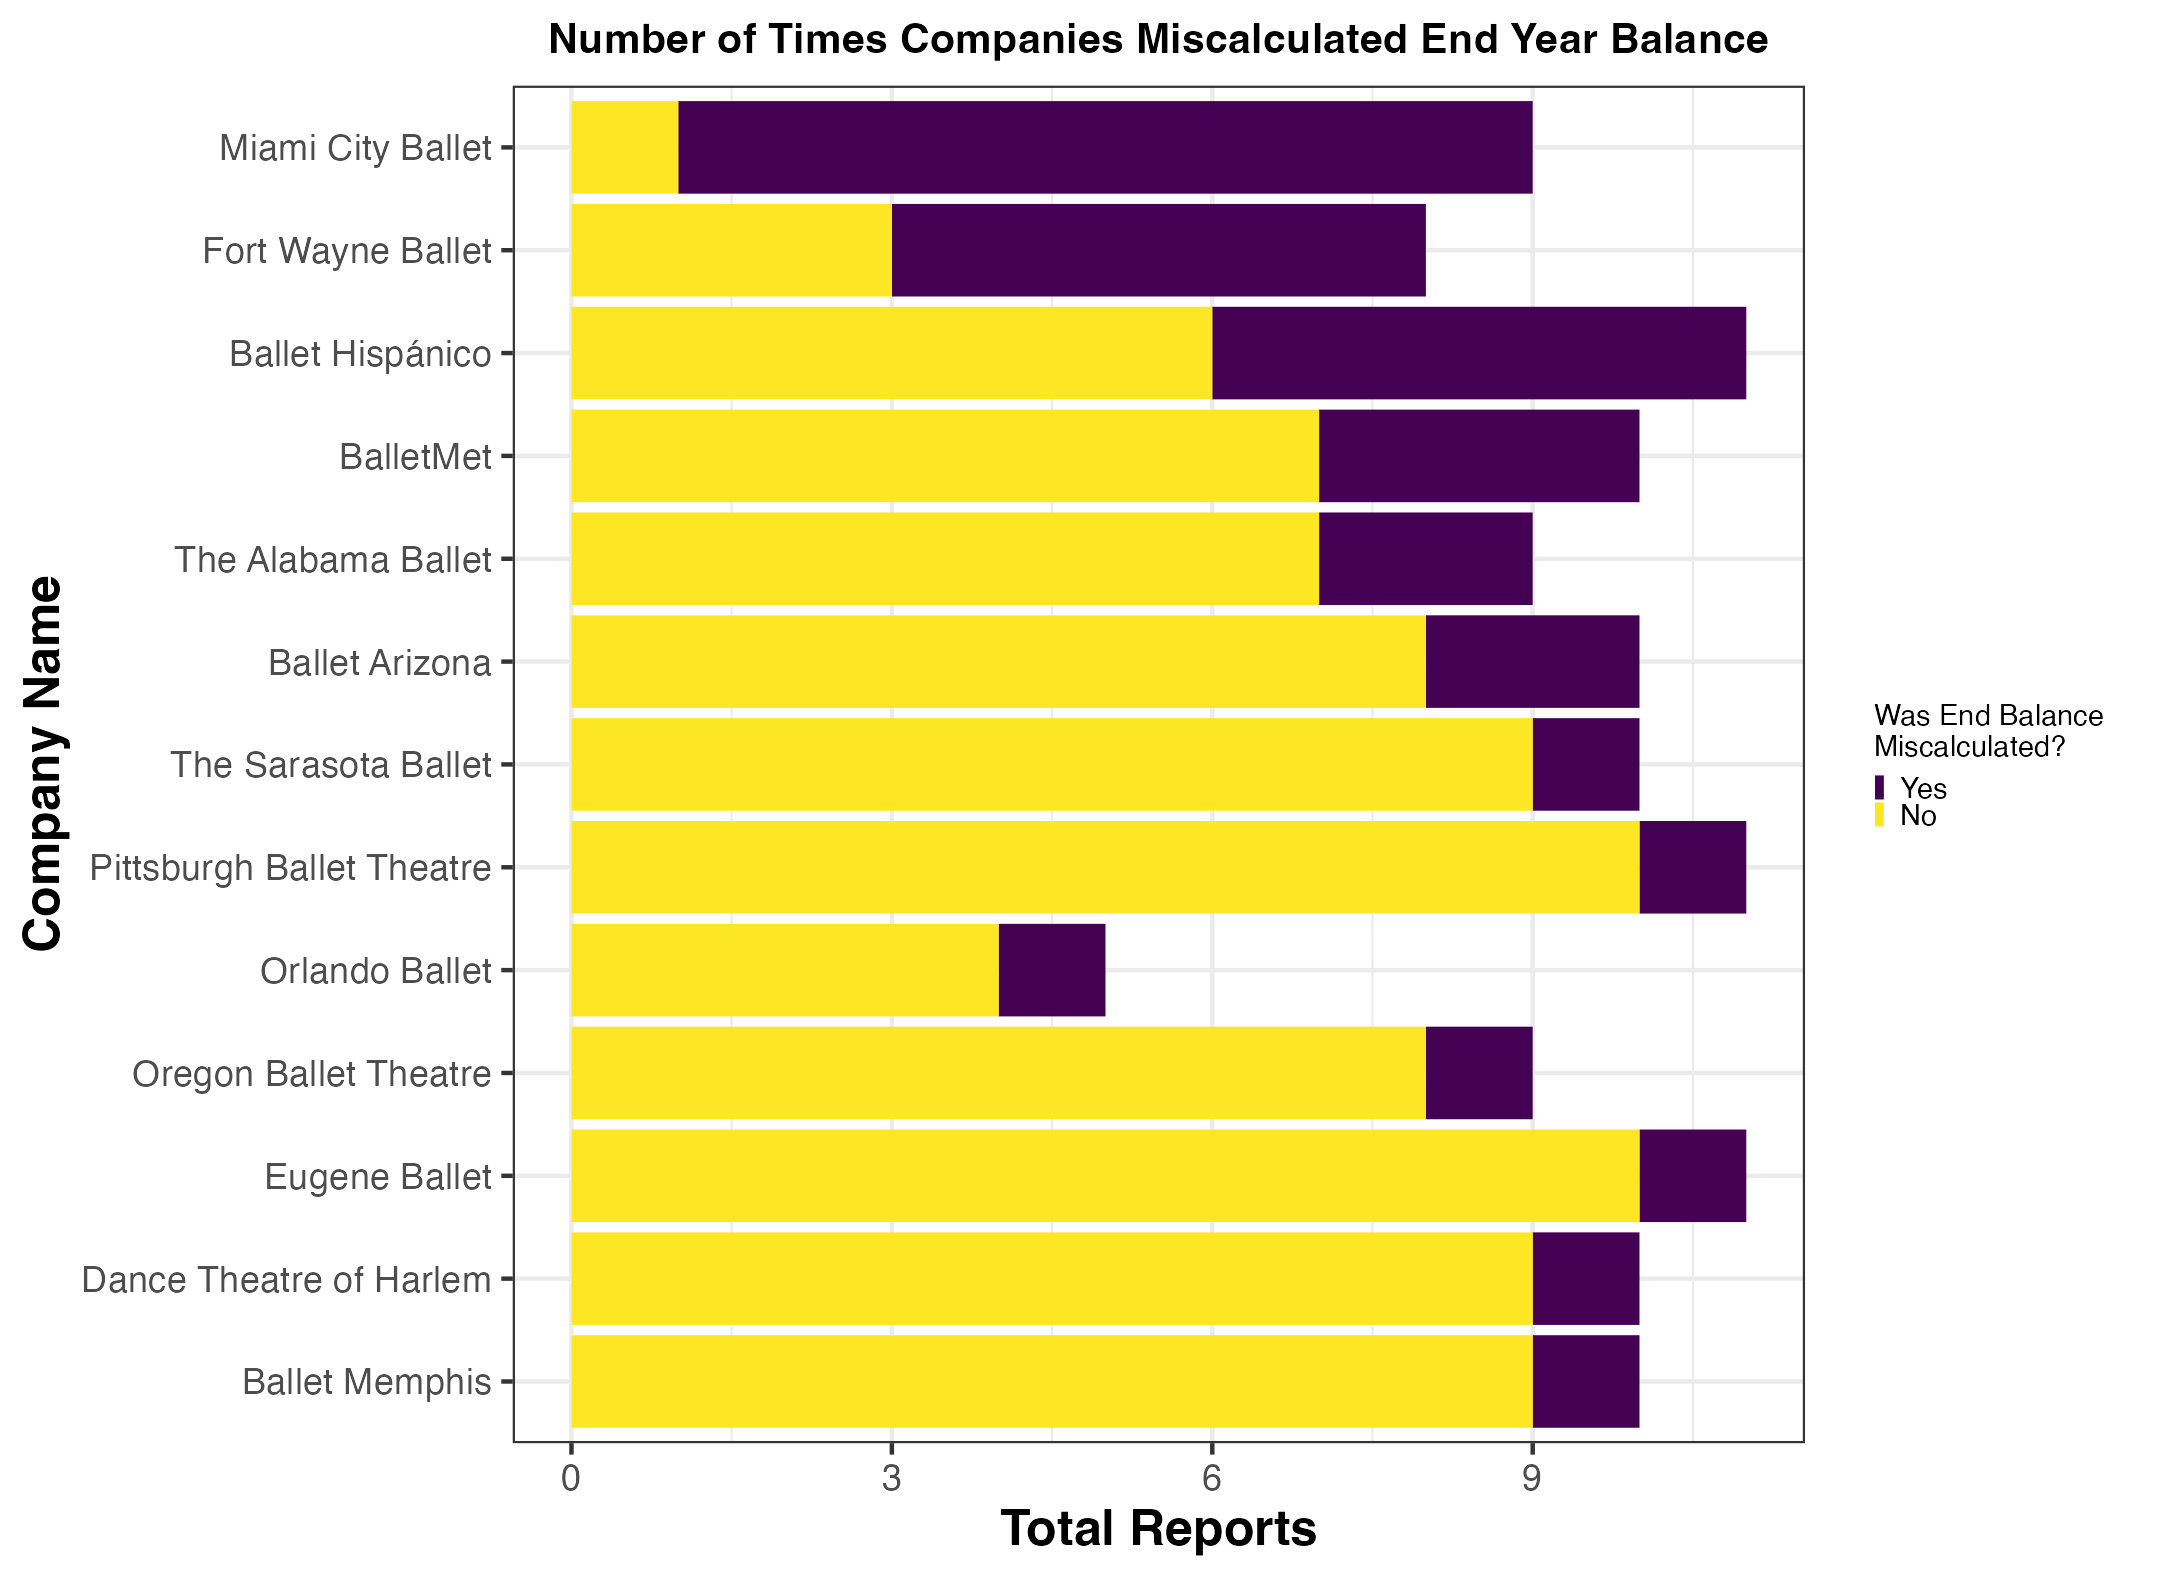
\includegraphics[width=0.5\linewidth,]{../images/miscalc_end_bal} \caption{\label{fig:miscalc-by-comp}Number of observations where there was a discrepancy between the calculated and reported end of year balance, using the absolute value equation given in equation (1).}\label{fig:miscalc-by-comp}
\end{figure}

\hypertarget{how-endowments-did-over-time}{%
\subsubsection{How Endowments Did Over
Time}\label{how-endowments-did-over-time}}

Annual percent change is the percent change from one value to the next
at the end of a year-long period. With regard to endowment balances, the
annual percent change in endowment balance is a comparison between the
endowment at the beginning of the fiscal year and the endowment of the
end of the fiscal year, which allows us to interpret by what percent the
endowment has grown or shrunk. Charting percent change over time allows
us to view endowment behavior over time; further, we can compare percent
changes between companies to get a sense for trends in how different
companies' endowments change.

To provide some context on the interpretation of percent change, we
first state a couple of standard definitions.

The relative change, which represents how much a value has changed
relative to its initial value, is

\[\text{Relative change} = \dfrac{\text{End Value} - \text{Start Value}}{ \text{Start Value}}.\]

The effect of considering relative change means that we can more easily
compare companies that have enormously different beginning of year
balance sizes. For a company with a small endowment, a difference of
10,000 may be substantial, while the same difference would be minimal if
the company has over a million in its endowment.

The percent change, which is the relative change in percentage form, is
simply \(\text{Relative Change} \times 100\).

When we are considering the percent change within a fiscal year, that
is, from the beginning of year balance to the end of year balance, a
couple of examples of the interpretation include\footnote{For a relative
  change of value \(R\), it can be more intuitive to interpret it by
  considering the expression
  \(\text{End Value} = (R+1) \times \text{Start Value}.\) That is, if we
  have a relative change, we simply add 1 to it and multiply it by the
  starting value to acquire the end value.}:

\begin{itemize}
\tightlist
\item
  If the percent change is \(-50\%\), the endowment's value at the end
  of the fiscal year is half of what it was at the beginning.
\item
  If the percent change is \(100\%\), the endowment's value at the end
  of the fiscal year is twice that it was at the beginning.\\
\item
  If the percent change is \(-100\%\), the endowment's value dropped to
  zero throughout the fiscal year.
\end{itemize}

We calculated each company's within-year percent change of endowment
balance, as this allows us to compare the performance of different
companies' endowments over time. A positive percent change indicates
growth within the fiscal year; a negative percent change indicates loss.

The percent change of most companies falls between -100\% and 200\%
(Figure \ref{fig:perc-change-endow}). There are notable outliers,
however, such as Joffrey Ballet in 2016 with a \textasciitilde3,000\%
increase (\ref{fig:perc-change-endow-all}). By focusing on lines between
-100\% and 200\%, we can see a trend appearing, with many companies
growing and shrinking at similar rates around similar times. Thus,
plotting the within-year percent change of the S\&P 500 as a proxy for
the stock market, we can see that many companies' endowment balances
reflect the performance of the stock market; this is unsurprising, given
the inherent invested nature of endowments. To assess companies' ``raw''
performance--in other words, how they managed their endowments outside
of their investment returns--we adjusted all percent changes for
investment earnings or losses, which flattened the stock market trend
(Figure \ref{fig:flat}). We use this flattened plot to investigate large
decreases and increases in endowment funds, as well as long term
behavior of endowments.

\begin{figure}[H]
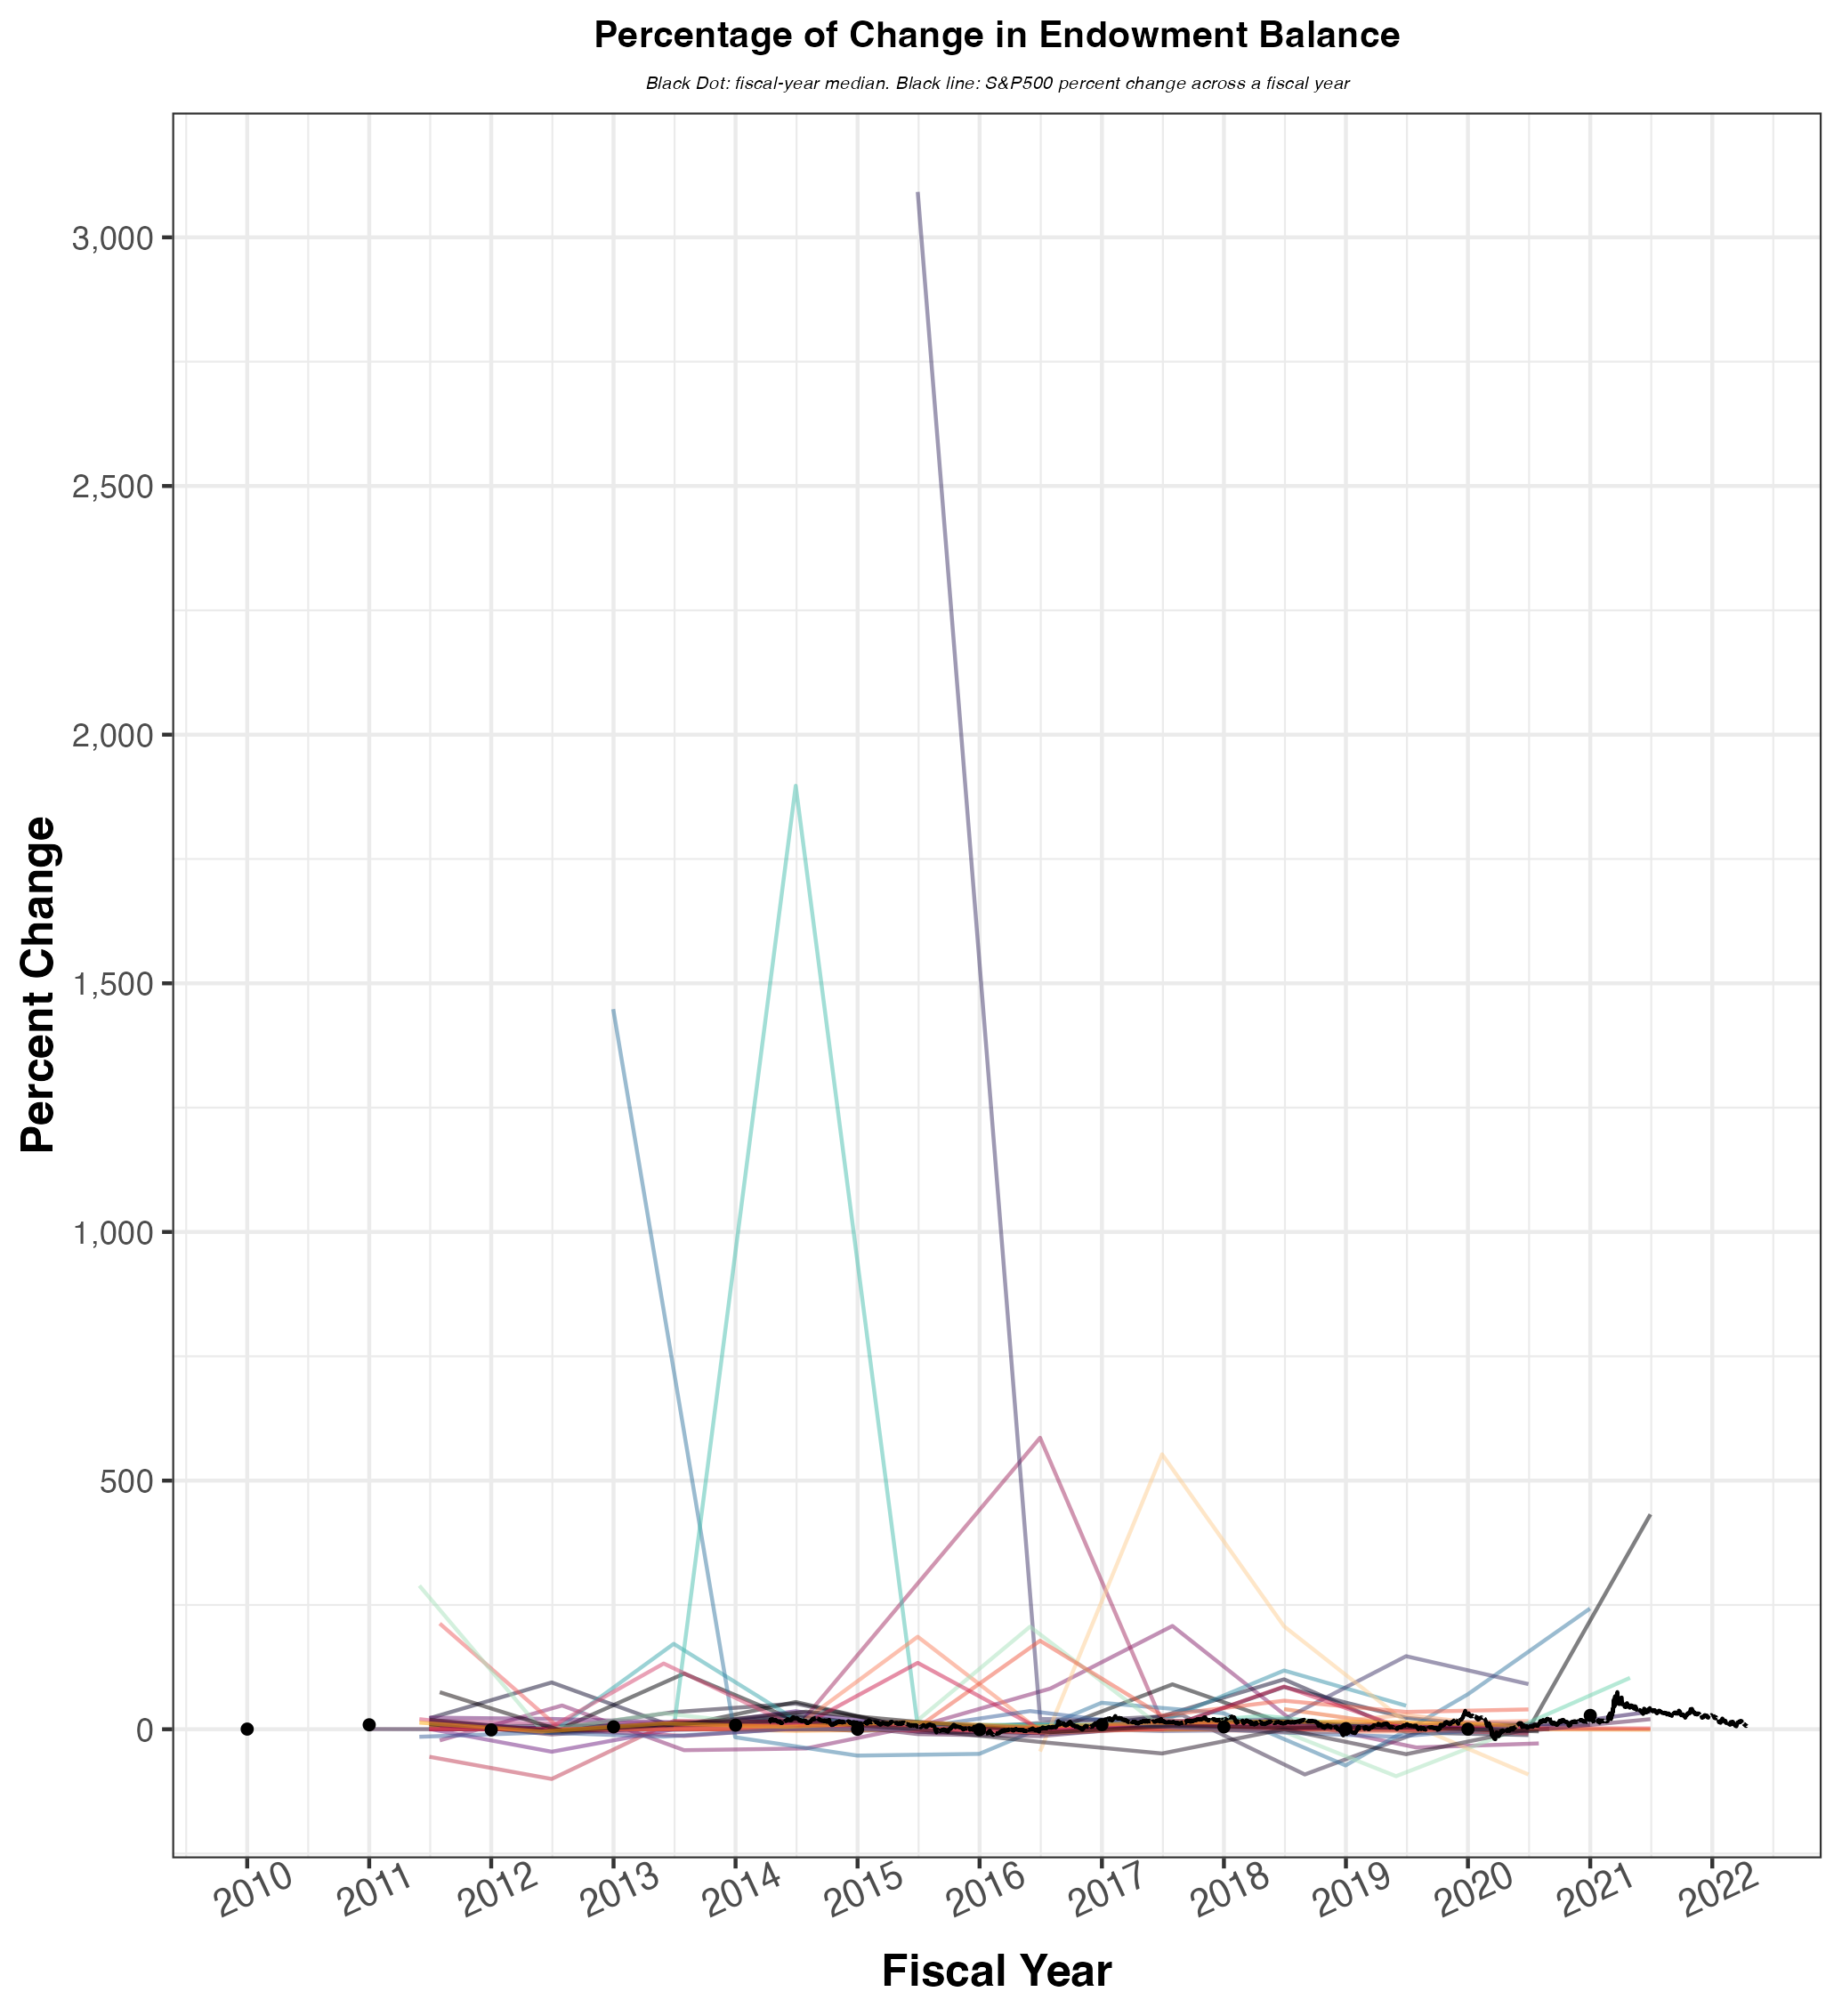
\includegraphics[width=0.8\linewidth,]{../images/pc_endow} \caption{\label{fig:perc-change-endow-all} Percent change in endowment balance over time, including the full range of percent changes, revealing several clear outliers.}\label{fig:unnamed-chunk-6}
\end{figure}

\begin{figure}[H]
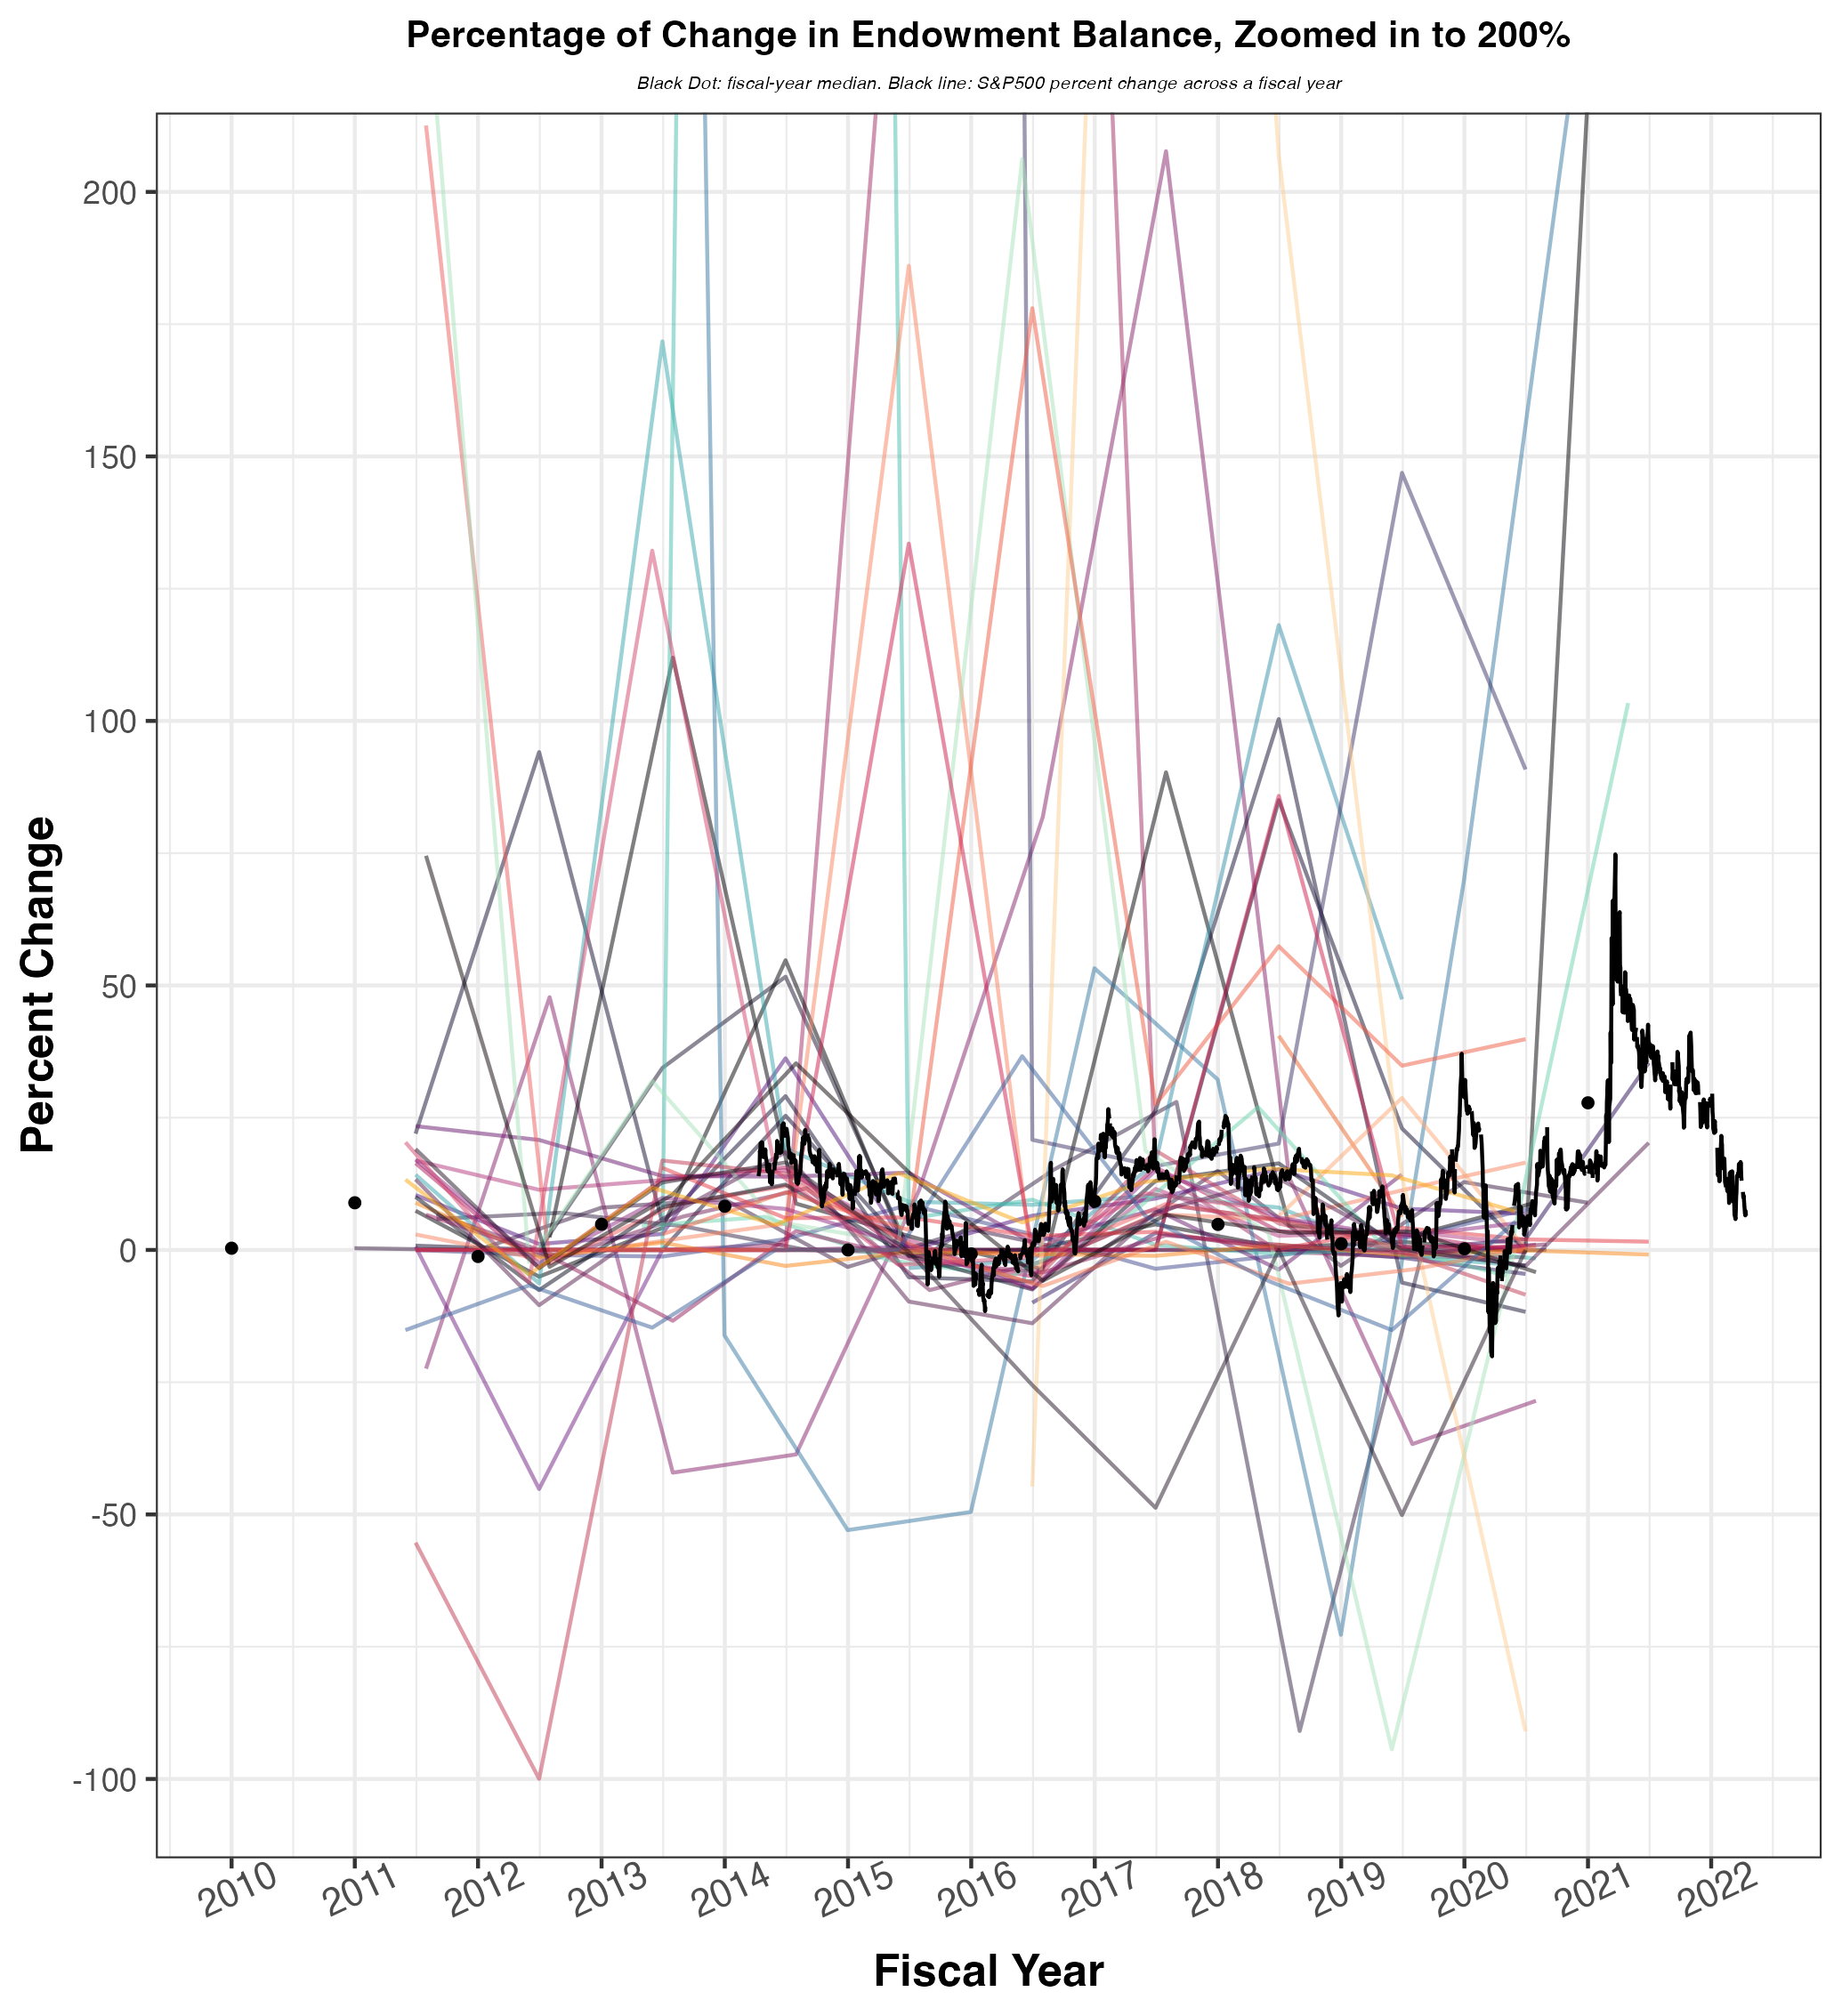
\includegraphics[width=0.8\linewidth,]{../images/pc_endow_zoom} \caption{\label{fig:perc-change-endow} Percent change in endowment balance over time, restricting the range to -200 percent to 200 percent to remove outliers than reduce our ability to see trends for the majority of companies.}\label{fig:unnamed-chunk-7}
\end{figure}

\begin{figure}[H]
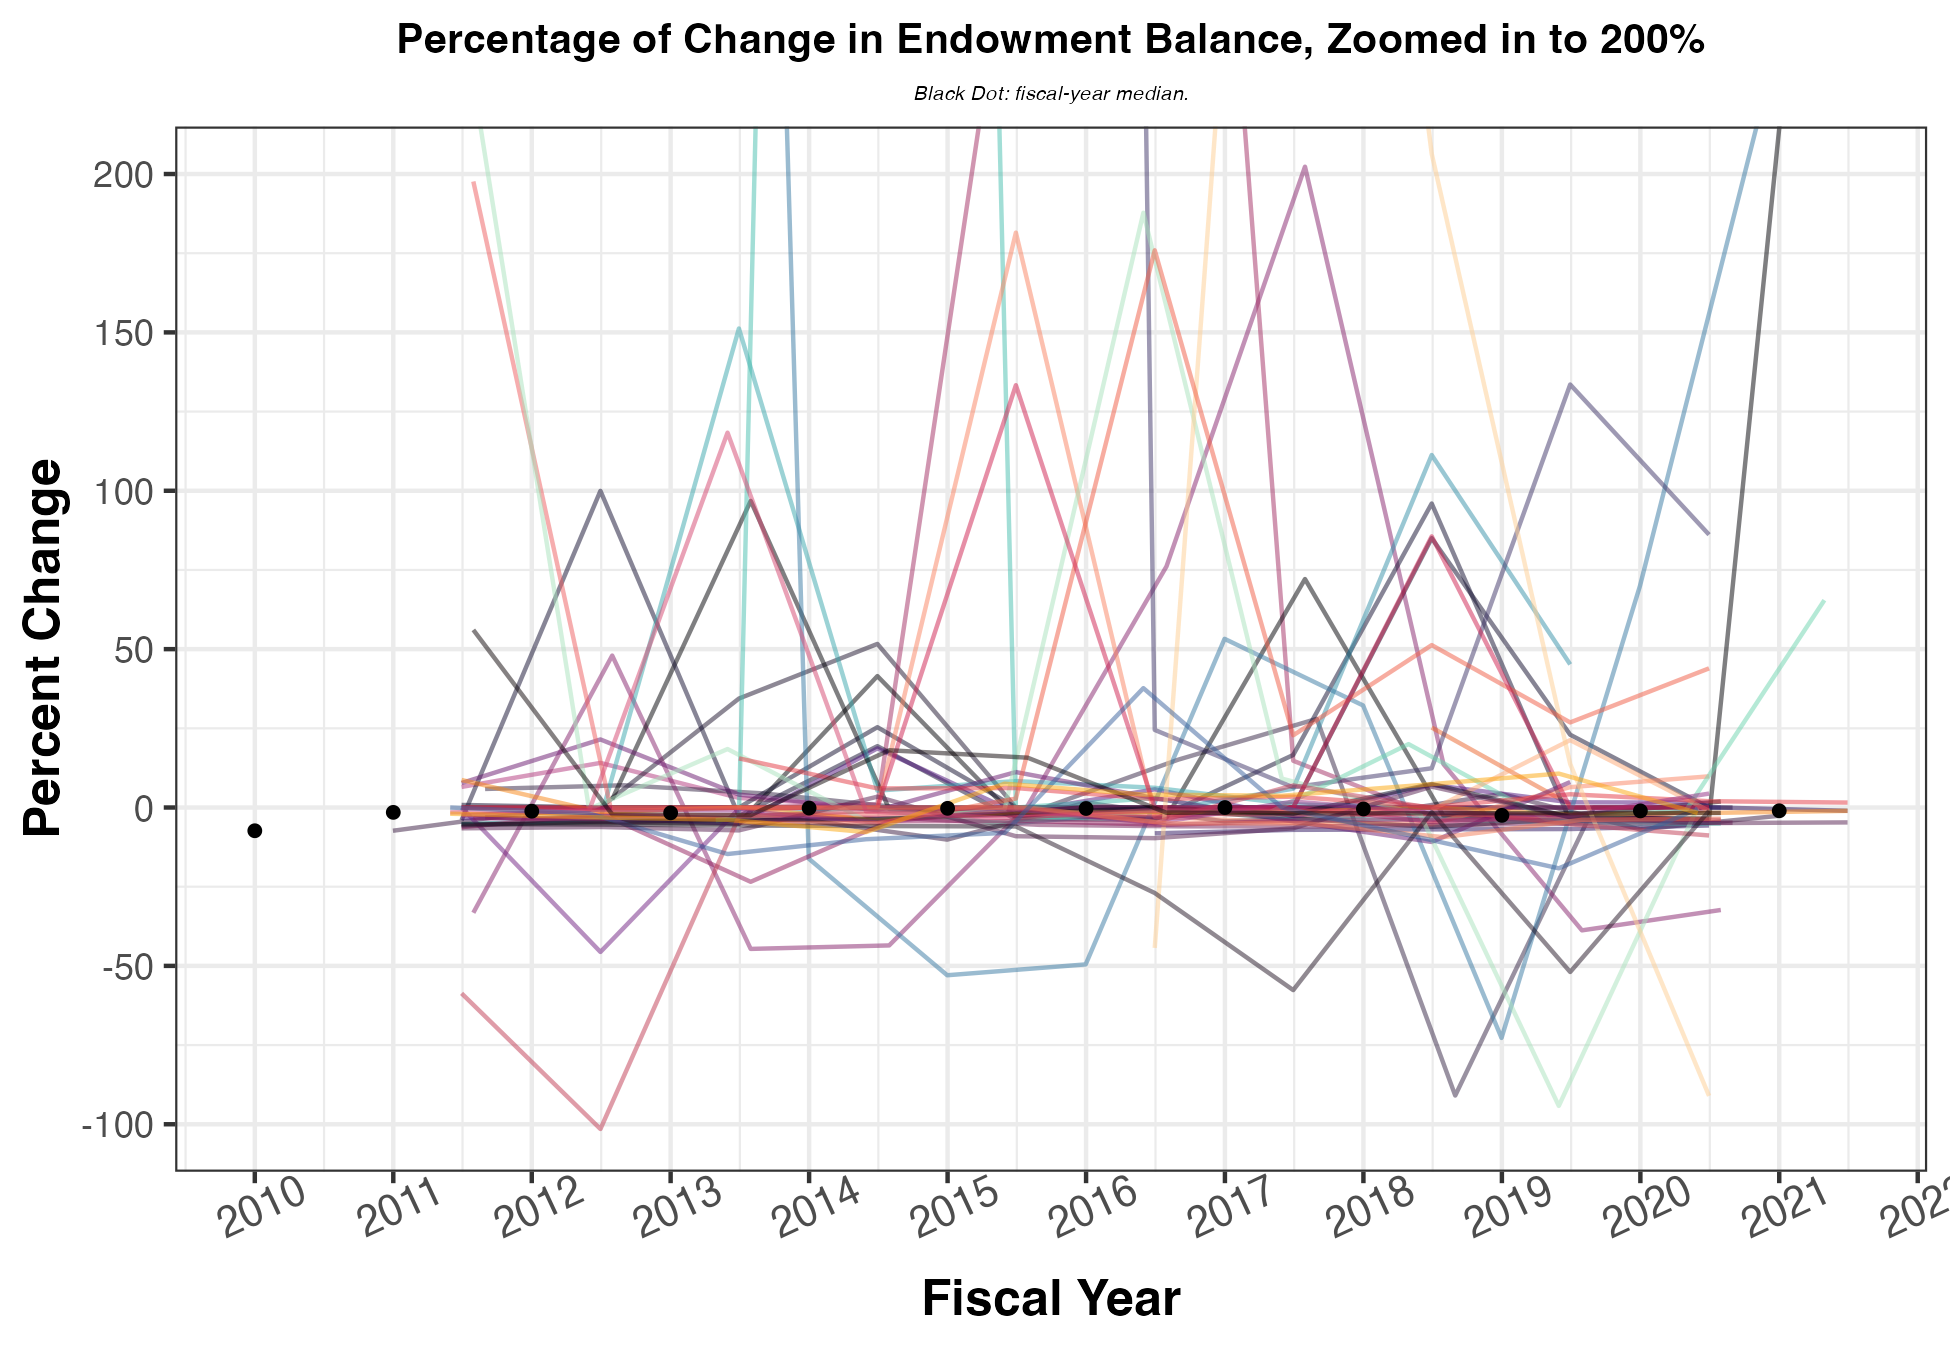
\includegraphics[width=0.8\linewidth,]{../images/pc_endow_flat} \caption{\label{fig:flat} Adjusting for investment earnings or losses when computing the endowment percent changes flattens the trends we see when using the unadjusted endowment values.}\label{fig:flat}
\end{figure}

Examining particular companies (Figure \ref{fig:below-40}), we can see
that eight companies reduce their endowment by over 40\% (e.g.~Percent
Change lower than -40\%) across multiple years. There are eight
companies that do so (Table 4) Aspen Santa Fe Ballet, Atlanta Ballet,
First State Ballet Theatre, Nashville Ballet, Orlando Ballet, San
Francisco Ballet, and The Washington Ballet. Some of these companies
reduce their endowments by over 40\% multiple times. While we cannot say
for certain why more companies have such severe reductions in endowment
balance, reductions can indicate a variety of situations for a company,
such as: dispersing their funds into a new fiscal entity\footnote{Aspen
  Santa Fe Ballet transferred most of their endowment into Aspen Santa
  Fe Ballet Endowment Inc in 2018, causing their 90\% reduction of
  funds.}, struggling financial in a given fiscal year, spending
newly-unrestricted funds, or purchasing large items such as a building.
Few companies severely reduce their endowment, thus the majority of US
dance companies with endowments are able to maintain their savings and
receive income from their endowments.

\begin{figure}[H]
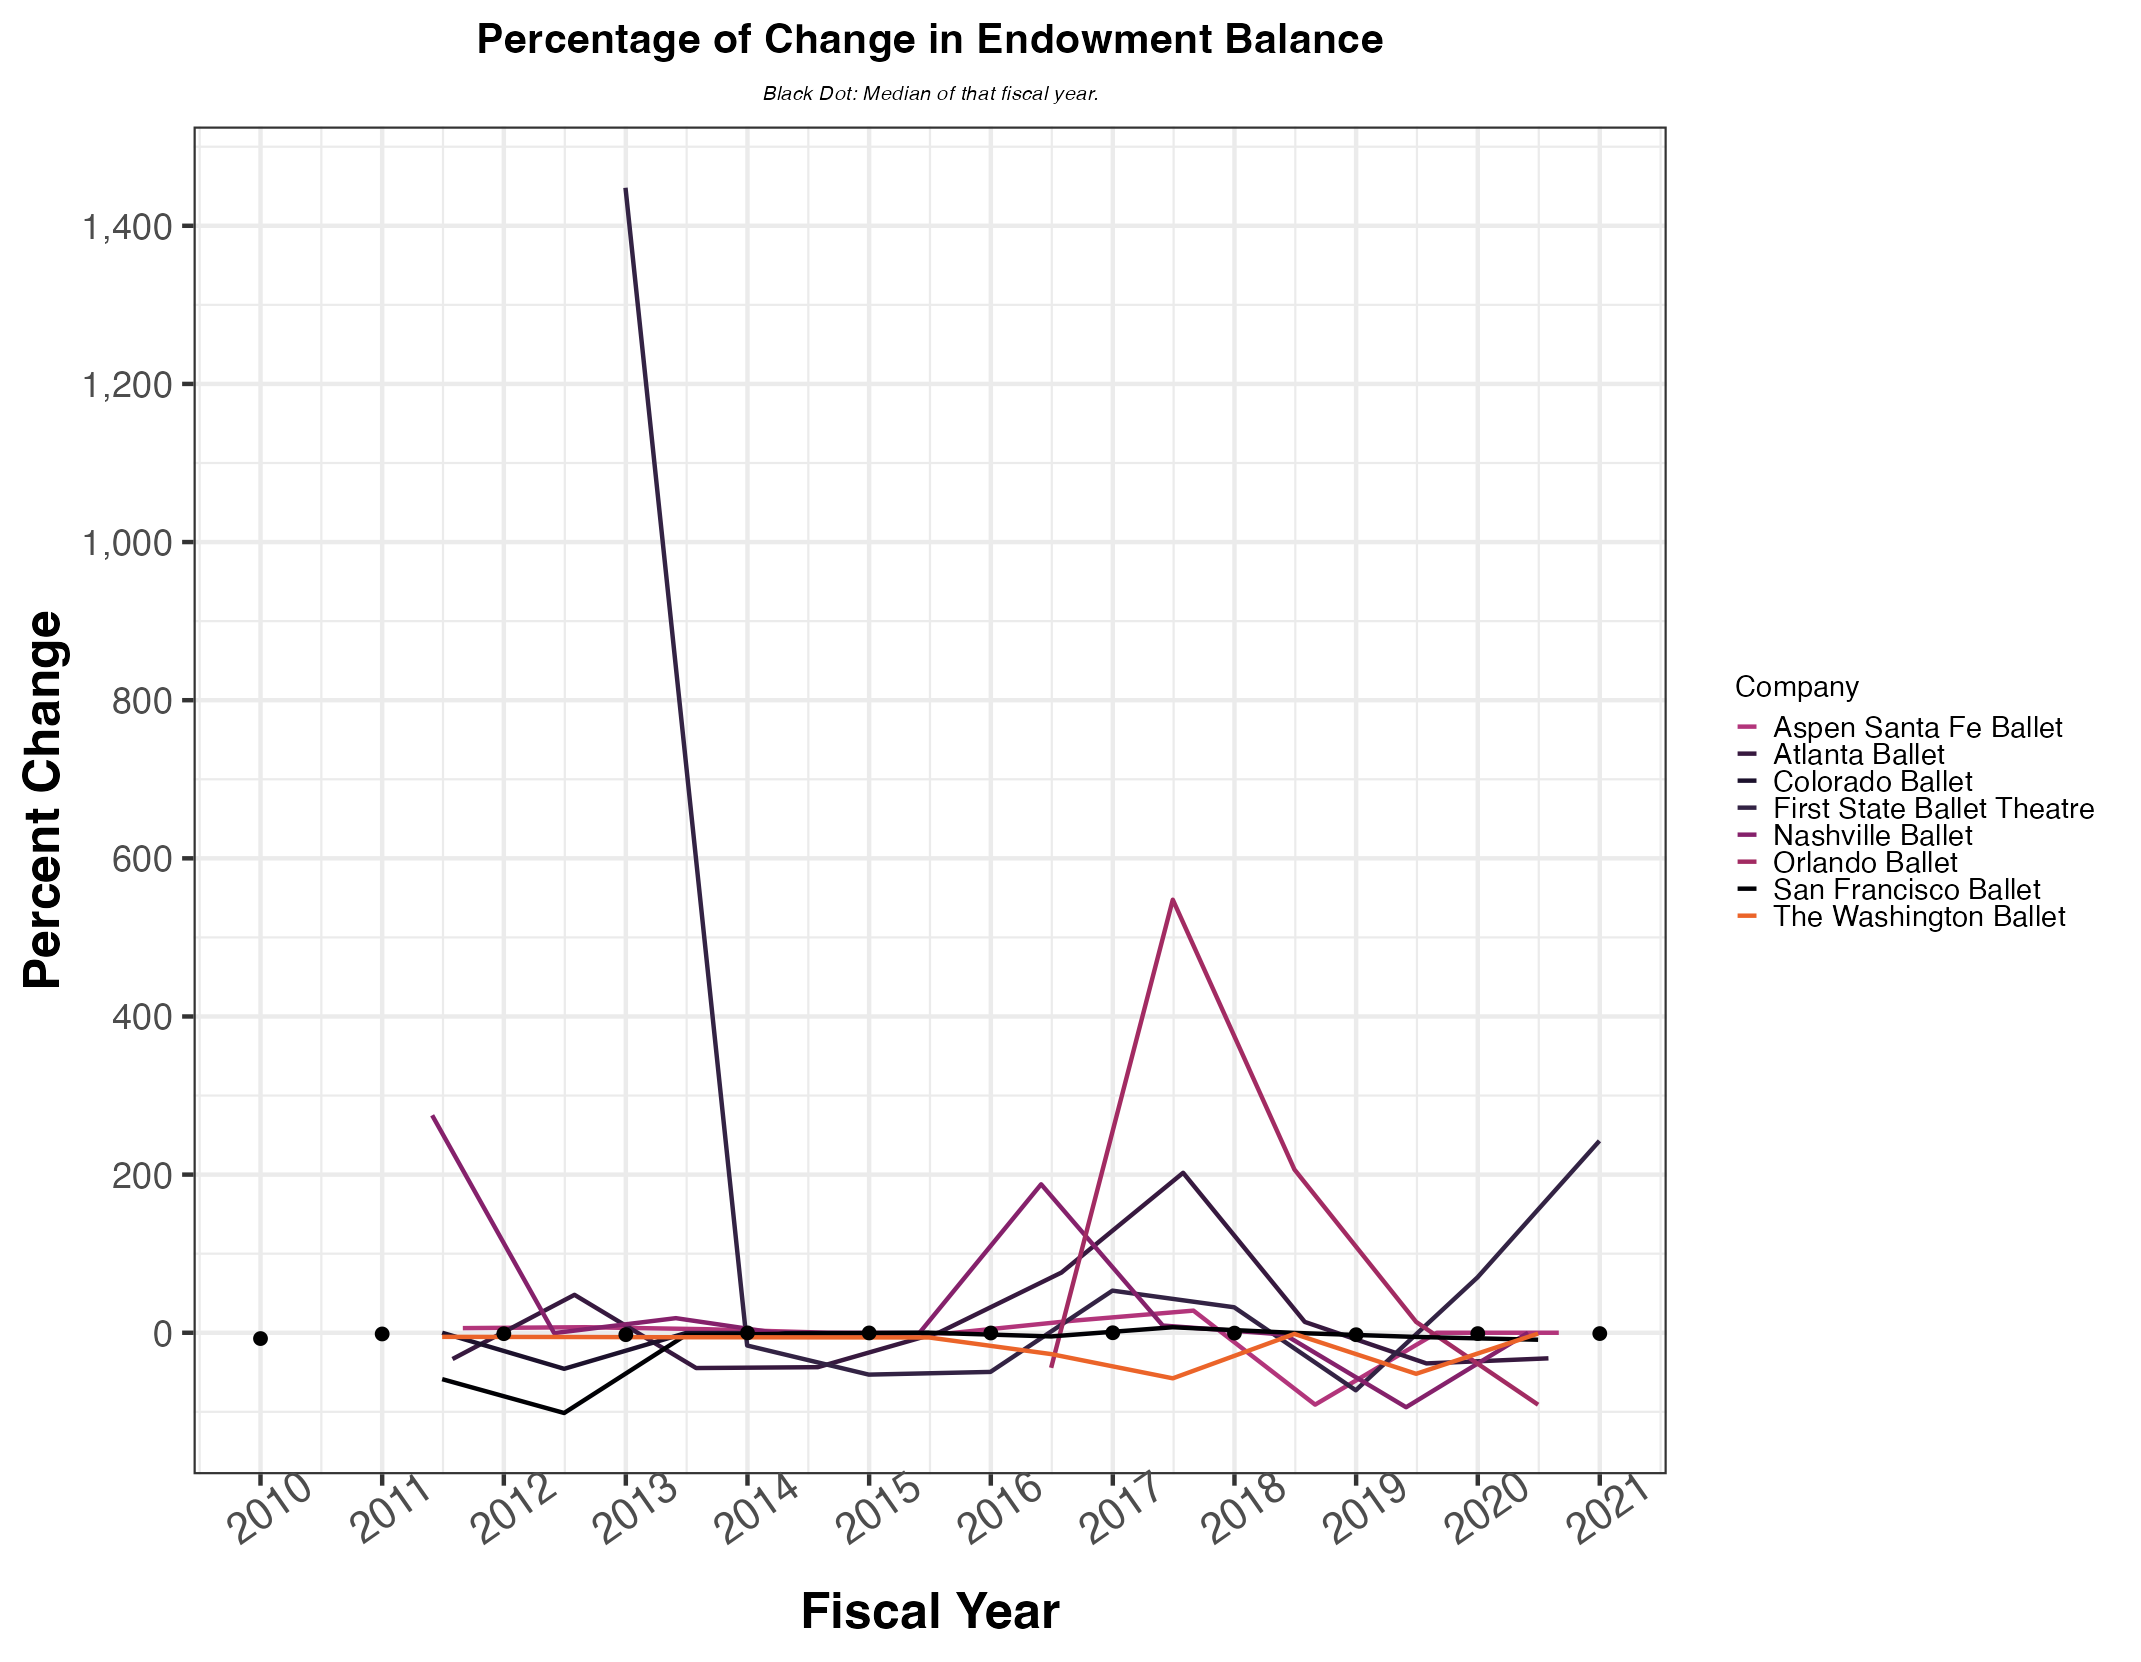
\includegraphics[width=0.8\linewidth,]{../images/pc_below_40} \caption{\label{fig:below-40} Companies that reduce their endowment by over 40 percent.}\label{fig:unnamed-chunk-8}
\end{figure}

\begin{table}[!h]

\caption{Endowment Percent Change Dropping Below 40 Percent Of Beginning Year balance}
\centering
\begin{tabular}[t]{lrrrr}
\toprule
Company Name & Percent Change & Beginning Balance & End Balance & Fiscal Year\\
\midrule
Aspen Santa Fe Ballet & -90.9 & 6065013 & 550000 & 2018\\
\addlinespace
Atlanta Ballet & -43.5 & 1706513 & 1046921 & 2014\\
\addlinespace
Atlanta Ballet & -44.6 & 2947203 & 1706513 & 2013\\
\addlinespace
Colorado Ballet & -45.6 & 182437 & 100000 & 2012\\
\addlinespace
First State Ballet Theatre & -72.7 & 36693 & 10000 & 2018\\
\addlinespace
First State Ballet Theatre & -49.5 & 35876 & 18107 & 2015\\
\addlinespace
First State Ballet Theatre & -53.0 & 76261 & 35876 & 2014\\
\addlinespace
Nashville Ballet & -94.2 & 1095624 & 61350 & 2019\\
\addlinespace
Orlando Ballet & -91.0 & 7732855 & 696082 & 2020\\
\addlinespace
Orlando Ballet & -44.3 & 613186 & 338943 & 2016\\
\addlinespace
San Francisco Ballet & -101.5 & 1035814 & 174 & 2012\\
\addlinespace
San Francisco Ballet & -58.7 & 2318646 & 1035814 & 2011\\
\addlinespace
The Washington Ballet & -51.9 & 621423 & 310000 & 2019\\
\addlinespace
The Washington Ballet & -57.6 & 1212247 & 621423 & 2017\\
\bottomrule
\end{tabular}
\end{table}

Additionally, we can see that eight companies increased their endowment
by over 200\% (percent Change higher than 200\%) across multiple years,
which means they at minimum tripled their endowment
(\ref{fig:above-200}). These eight companies are: Atlanta Ballet, Ballet
Arizona, Ballet Hispánico, First State Ballet Theatre, Fort Wayne
Ballet, Joffrey Ballet, Nashville Ballet, and Orlando Ballet. Such
dramatic increases are potentially indicative of large donations,
liquidation of assets such as buildings, or aggregation of funds from
separate endowment accounts.

\begin{figure}[H]
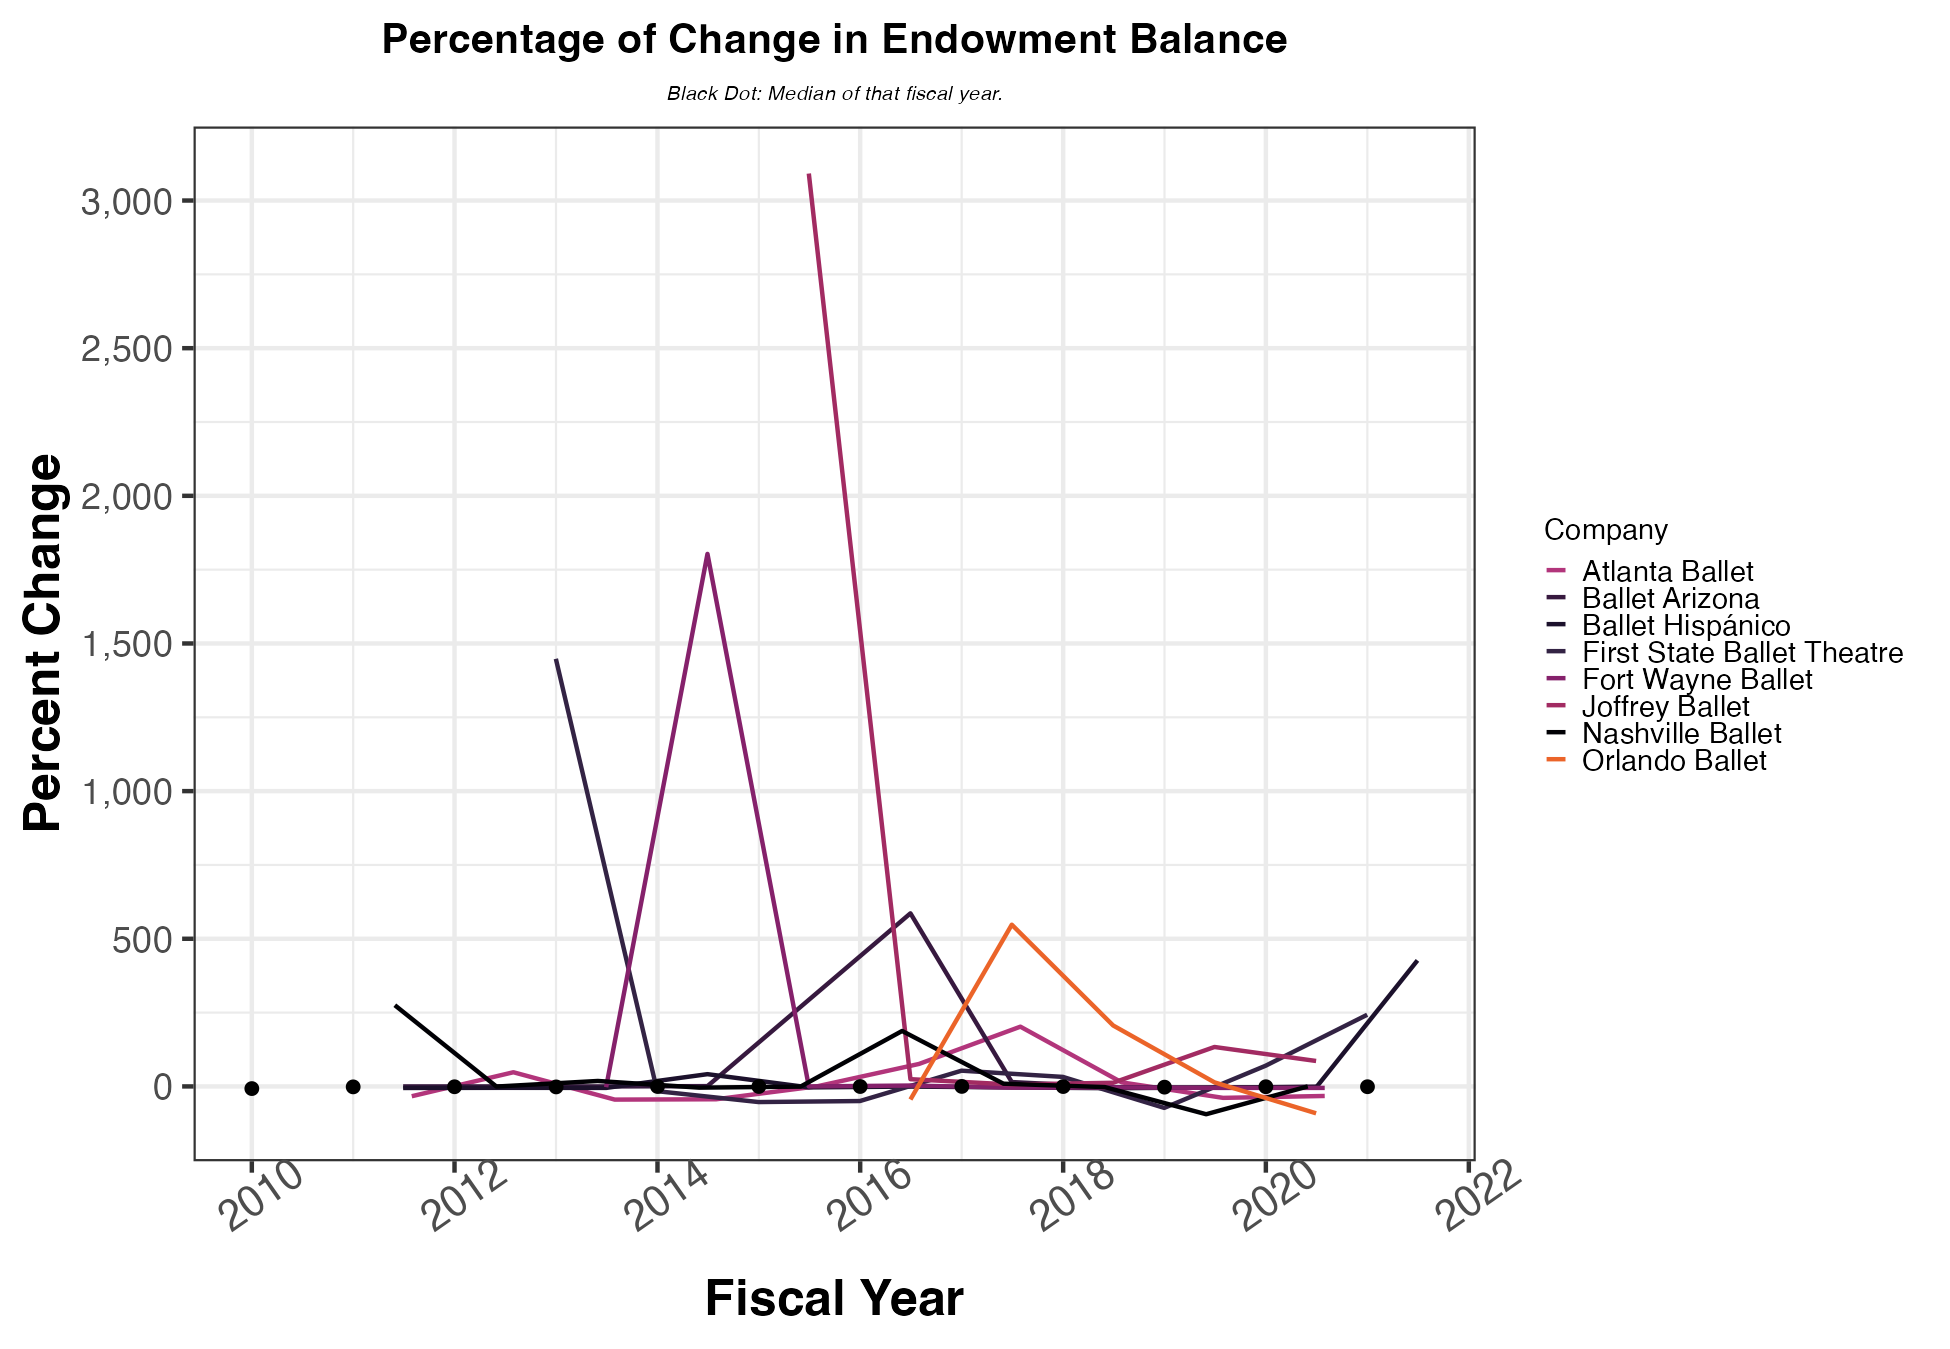
\includegraphics[width=0.9\linewidth,]{../images/pc_above_200} \caption{\label{fig:above-200} Annual percent change for companies that increased their endowment over 200 percent.}\label{fig:unnamed-chunk-9}
\end{figure}

\begin{table}

\caption{Endowment Percent Change Increasing Beyond 200 Percent Of Beginning Year Balance}
\centering
\begin{tabular}[t]{lrrrr}
\toprule
Company Name & Percent Change & Beginning Balance & End Balance & Fiscal Year\\
\midrule
Atlanta Ballet & 202.3 & 2119967 & 6523144 & 2017\\
\addlinespace
Ballet Arizona & 586.1 & 601399 & 4126424 & 2016\\
\addlinespace
Ballet Hispánico & 426.8 & 1405952 & 7481852 & 2021\\
\addlinespace
First State Ballet Theatre & 242.7 & 16999 & 58253 & 2020\\
\addlinespace
First State Ballet Theatre & 242.7 & 16999 & 58253 & 2020\\
\addlinespace
First State Ballet Theatre & 1448.1 & 5874 & 90934 & 2012\\
\addlinespace
Fort Wayne Ballet & 1803.3 & 60137 & 1201082 & 2014\\
\addlinespace
Joffrey Ballet & 3091.4 & 35600 & 1136139 & 2015\\
\addlinespace
Nashville Ballet & 275.0 & 54543 & 212030 & 2011\\
\addlinespace
Orlando Ballet & 206.4 & 2212808 & 6791249 & 2018\\
\addlinespace
Orlando Ballet & 547.7 & 338943 & 2212808 & 2017\\
\bottomrule
\end{tabular}
\end{table}

To examine the behavior of endowments, we ranked each company by its
consistency over time. We define consistency by ranking companies by
their standard deviation of a company's percent change across all years
on file. The smaller the standard deviation, the more consistent the
company's endowment behavior was, thus the higher the rank. (Figure
\ref{fig:pc-consist}). We find that many companies who have consistent
balances tend to not make large adjustments to their percent change.
Further, consistency in endowment does not appear to be related to
company size (Figure \ref{fig:endo-size}), as measured by both endowment
total balance and number of employees.

\begin{figure}[H]
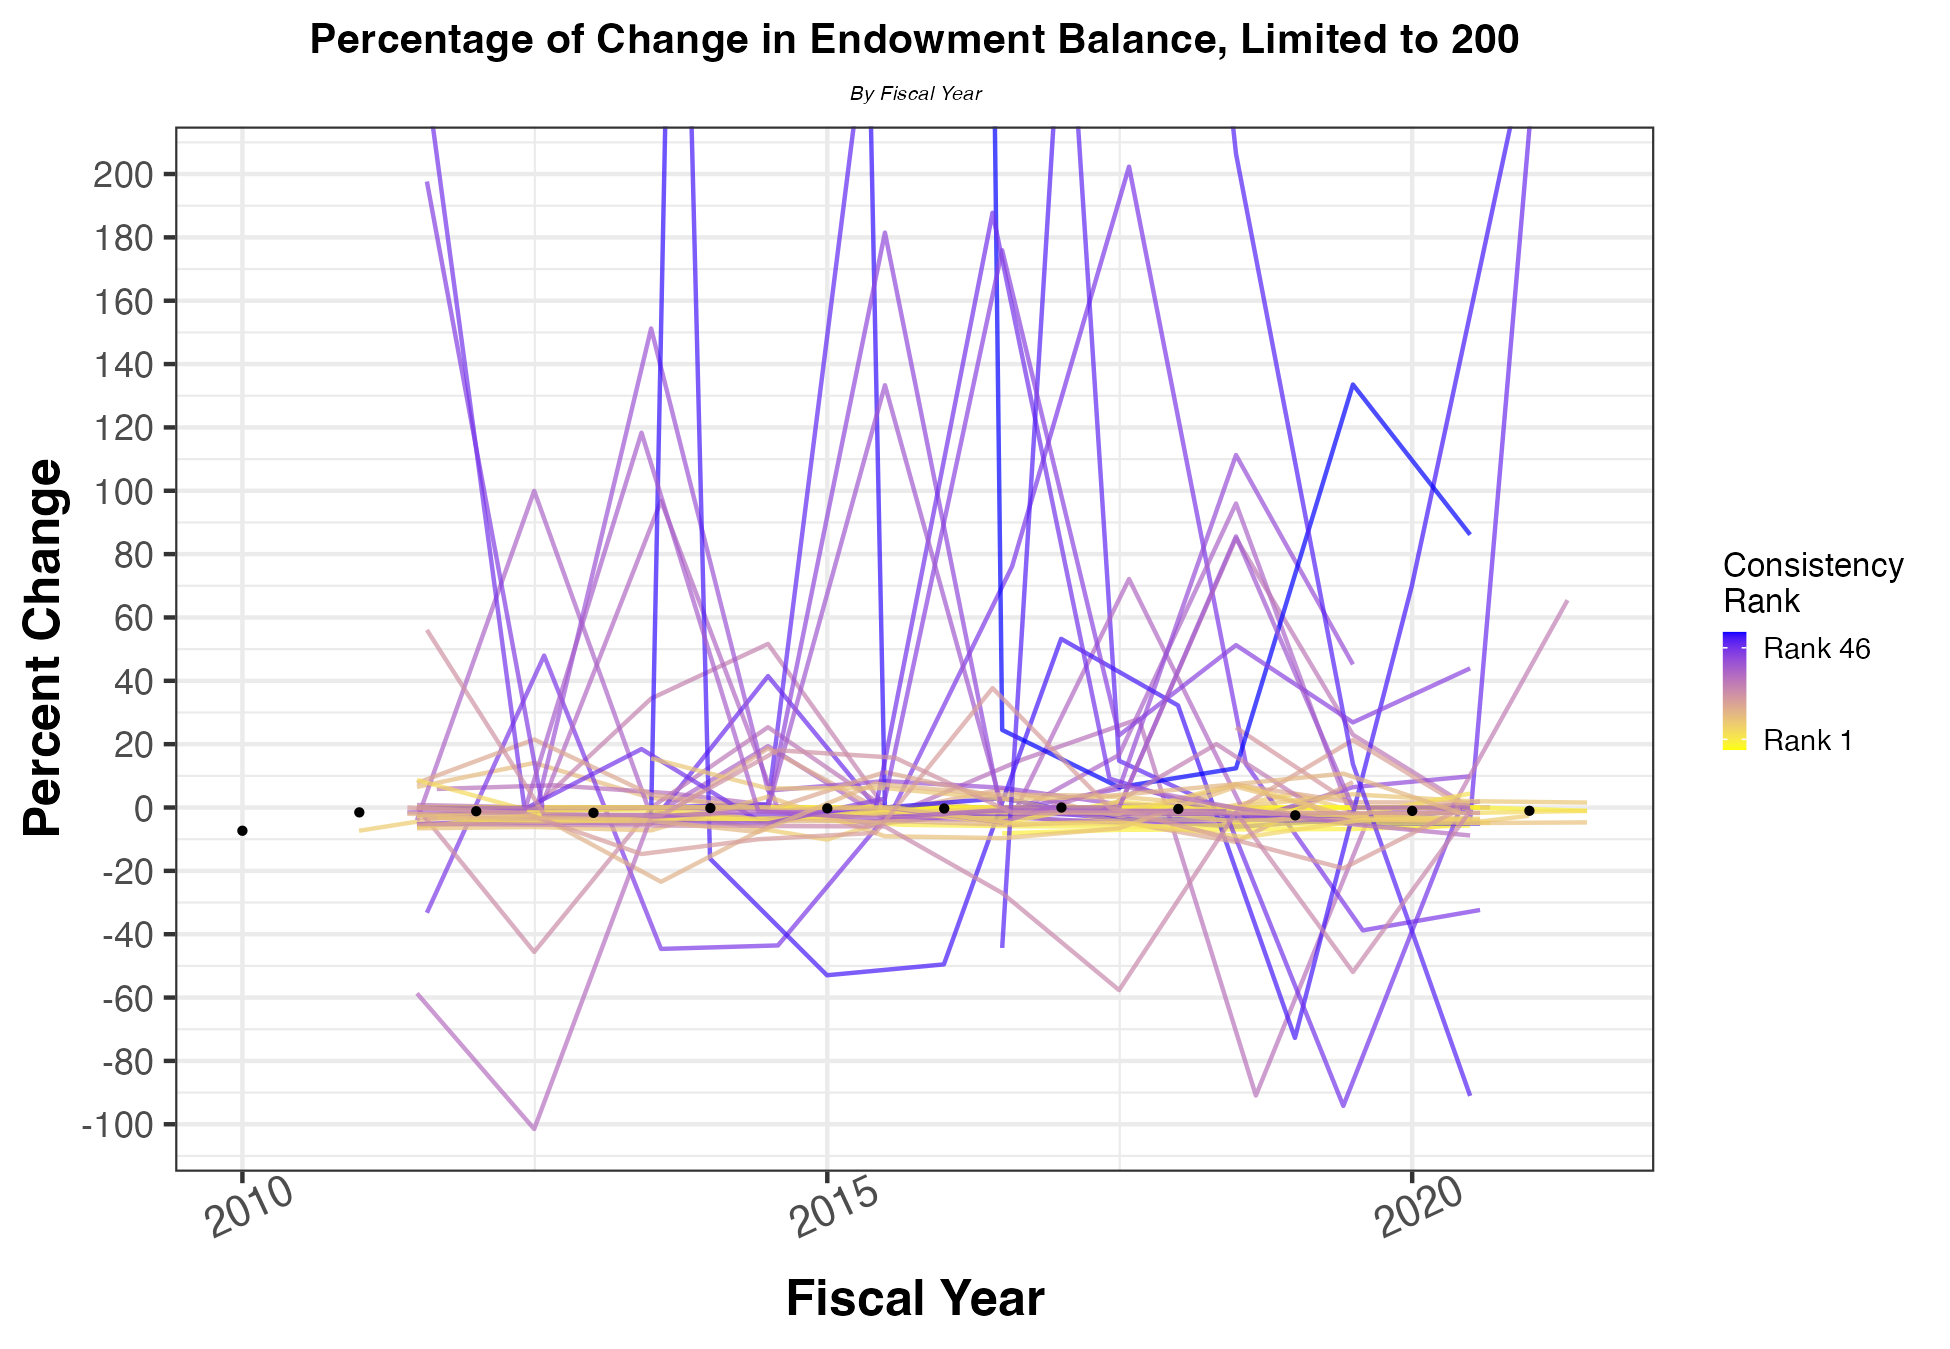
\includegraphics[width=0.9\linewidth,]{../images/pc_consist} \caption{\label{fig:pc-consist}}\label{fig:unnamed-chunk-10}
\end{figure}

\begin{figure}[H]
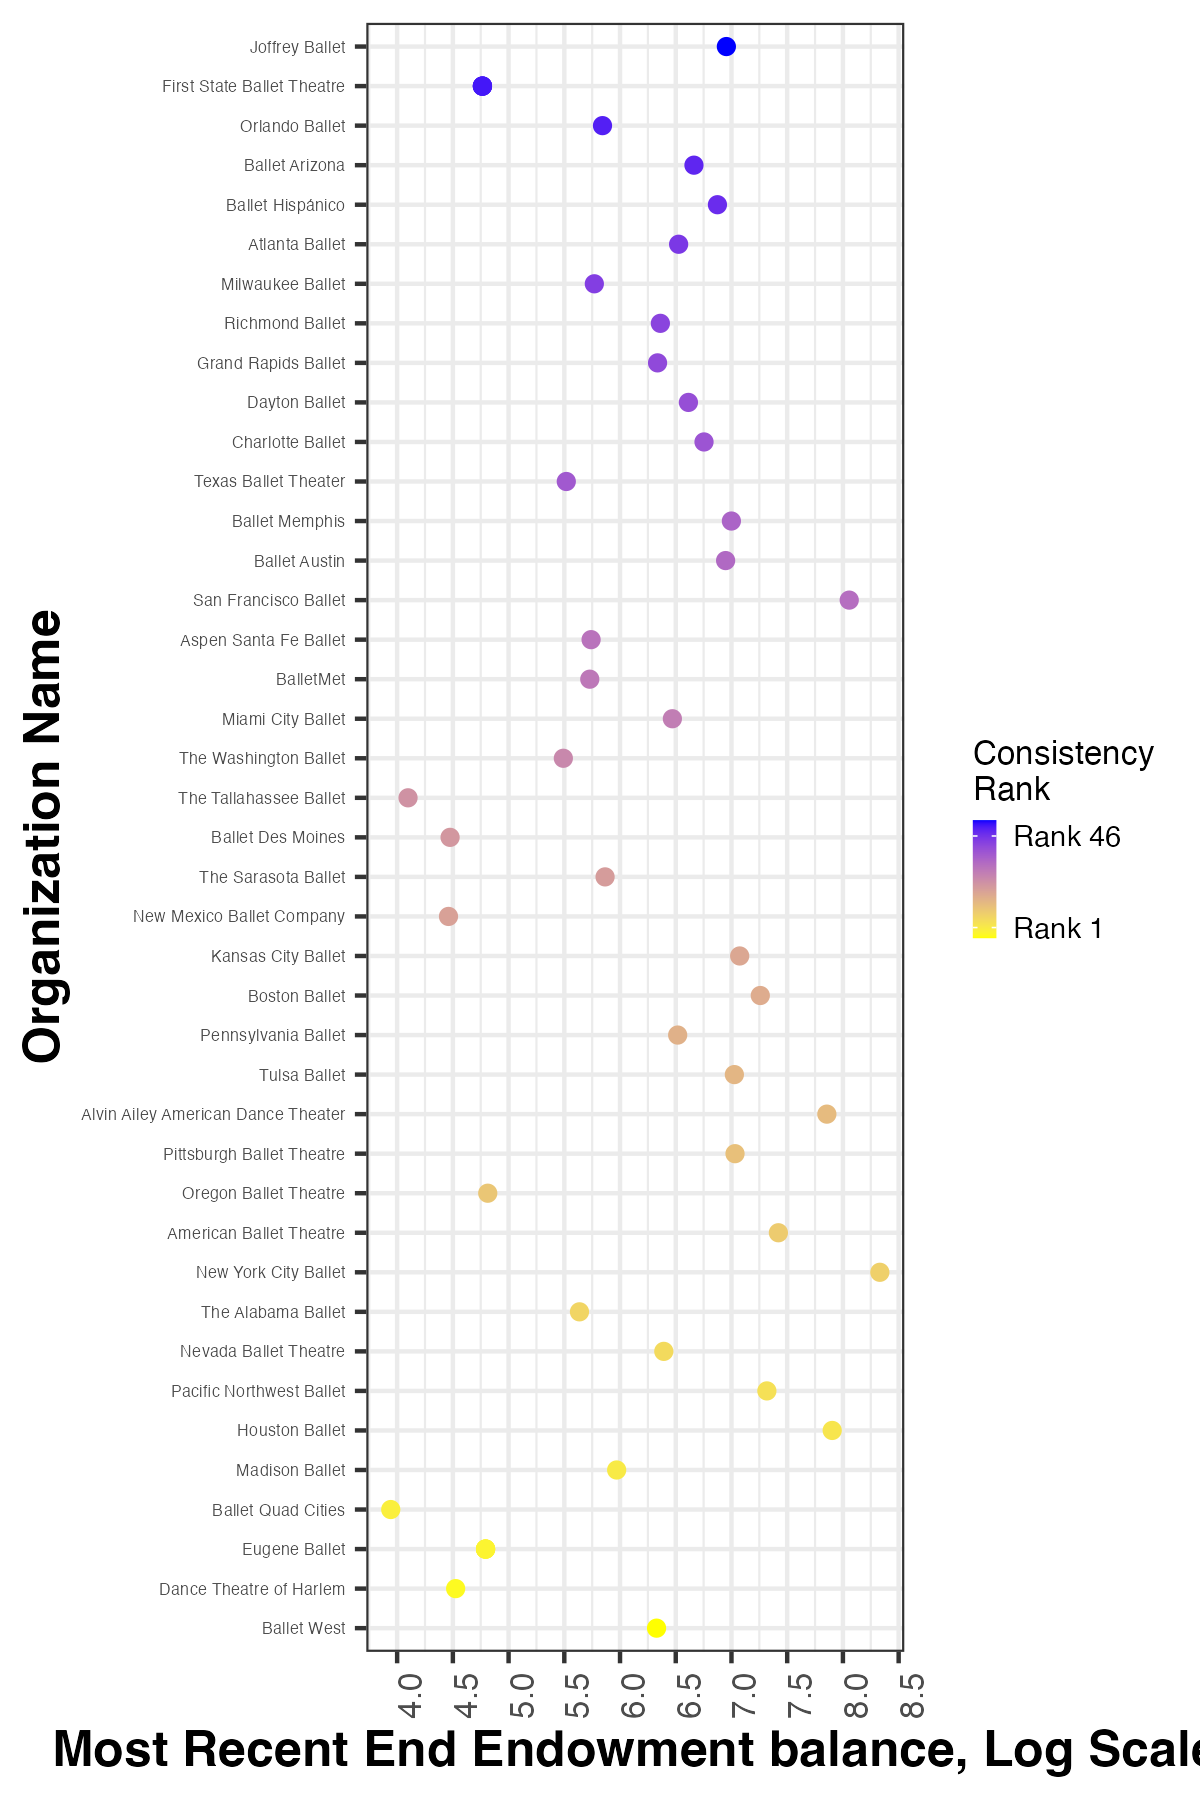
\includegraphics[width=0.5\linewidth,]{../images/consist_by_endo_size} 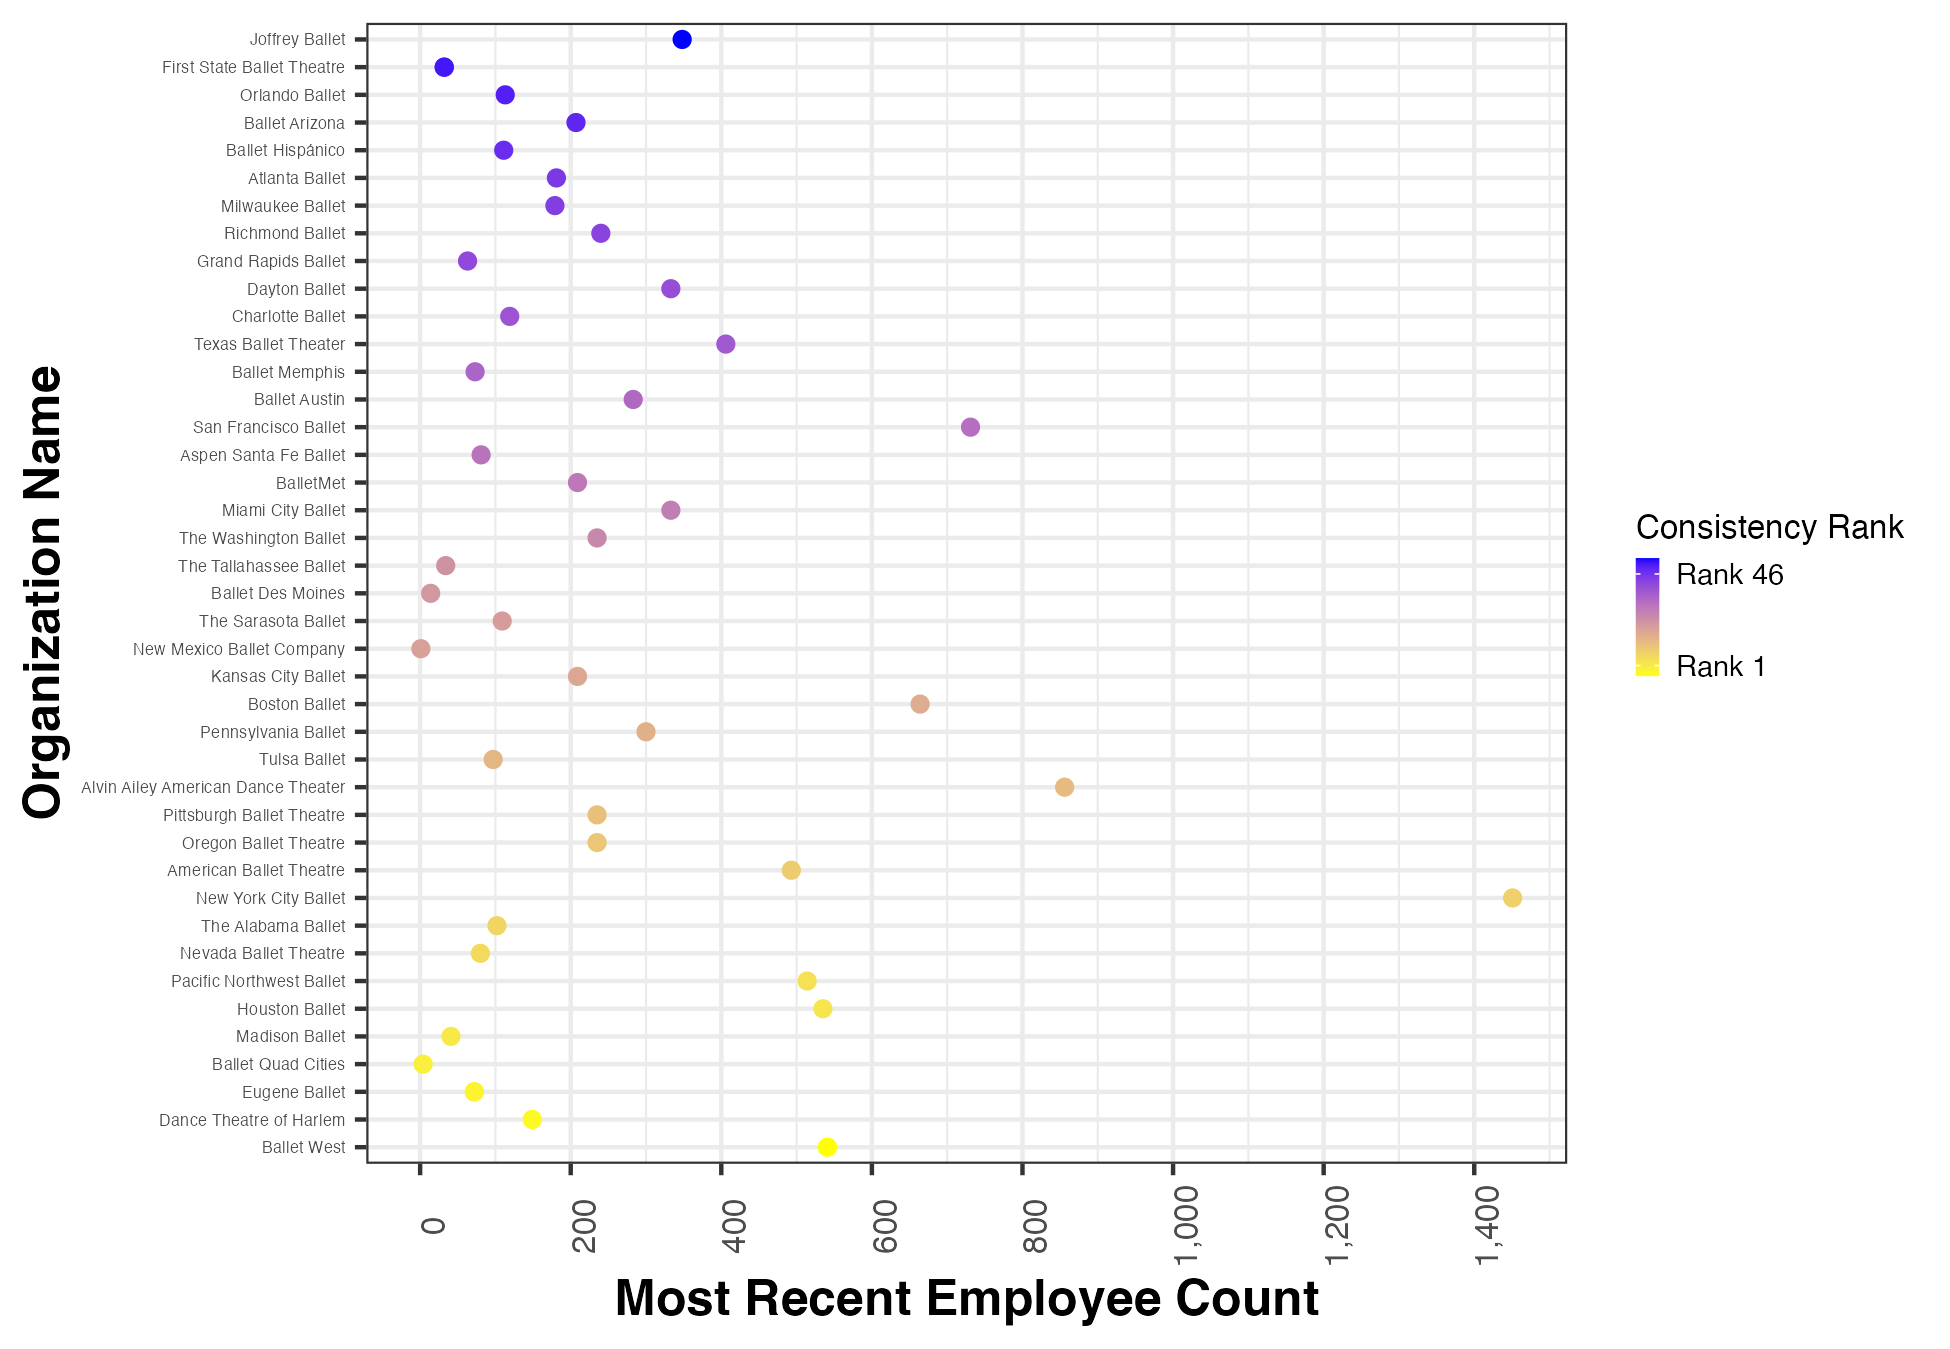
\includegraphics[width=0.5\linewidth,]{../images/consist_by_employ_count} \caption{\label{fig:endo-size}}\label{fig:unnamed-chunk-11}
\end{figure}

\hypertarget{compound-annual-growth-rate}{%
\subsubsection{Compound Annual Growth
Rate}\label{compound-annual-growth-rate}}

The compound annual growth rate is a useful way to summarize the
performance of different endowments over the same time period, since the
variability in annual growth rates can make it difficult to see broader
trends. We can think of this rate where, if the value grew by this same
rate each year, would give us the end value at the end of the time
period considered.

When we look at compound annual growth rate in this setting, we want to
account for withdrawals and contributions to separate how endowments are
doing due to investment decisions versus how they change due to large
contributions or withdrawals.

The basic formula for the compound growth rate over \(t\) years is

\[{\text{Compound Annual Growth Rate} = \left( \frac{\text{End Value}}{\text{Beginning Value}}\right)^{\frac{1}{t}}-1}.\]

Withdrawals as reported on the 990 include other expenditures, grants
and scholarships, and administrative expenses.

This means we can compute the withdrawals for any given year and company
as

\[\small{\text{Withdrawals} = \text{Other Expenditures} +\text{Administrative Expenses} +\text{Administrative Expenses} + \text{Grants and Scholarships}}.\]

To adjust for contributions and expenditures, we define the Compound
Annual Growth Rate as
\[{\left( \frac{\text{End Value} + \sum_{i=1}^{t-1} \text{Withdrawals} - \sum_{i=1}^{t-1} \text{Contributions}  }{\text{Beginning Value}} \right)^{\frac{1}{t}}-1}.\]

Adding back the withdrawals and subtracting off the contributions allows
us to see differences that are due specifically to investment choices.
Otherwise, we would not be able to tell whether a large increase in
endowment funds in a particular year was due to investment gains or a
large contribution.

In Figure \ref{fig:compound-growth}, we compare the compound growth
rates of the companies to the compound growth rate of the S\&P 500 over
the same time period, where we use the S\&P 500 as a benchmark to
indicate how the stock market is doing overall. Variations in the S\&P
500 across companies for a given time interval are due to differences in
their fiscal years. While Ballet Arizona and San Francisco have enormous
differences when considering the time intervals 2011 to 2020 and 2015 to
2020, it is unclear whether these changes are truly this large in
magnitude or if the differences are due to discrepancies in reporting.
Although we reached out to both companies to clarify discrepancies in
early years, we received no reply.

A substantial proportion (about 40\% of the companies for the 2011-2020
time period, and about 50\% of companies for the 2015-2020 and 2017-2020
time periods) had a compound annual growth rate less than 0.05\%. We see
the same concept at a more granular level considering the annual growth
rates in Figure \ref{fig:annual-growth-endowment}.

\begin{figure}[H]
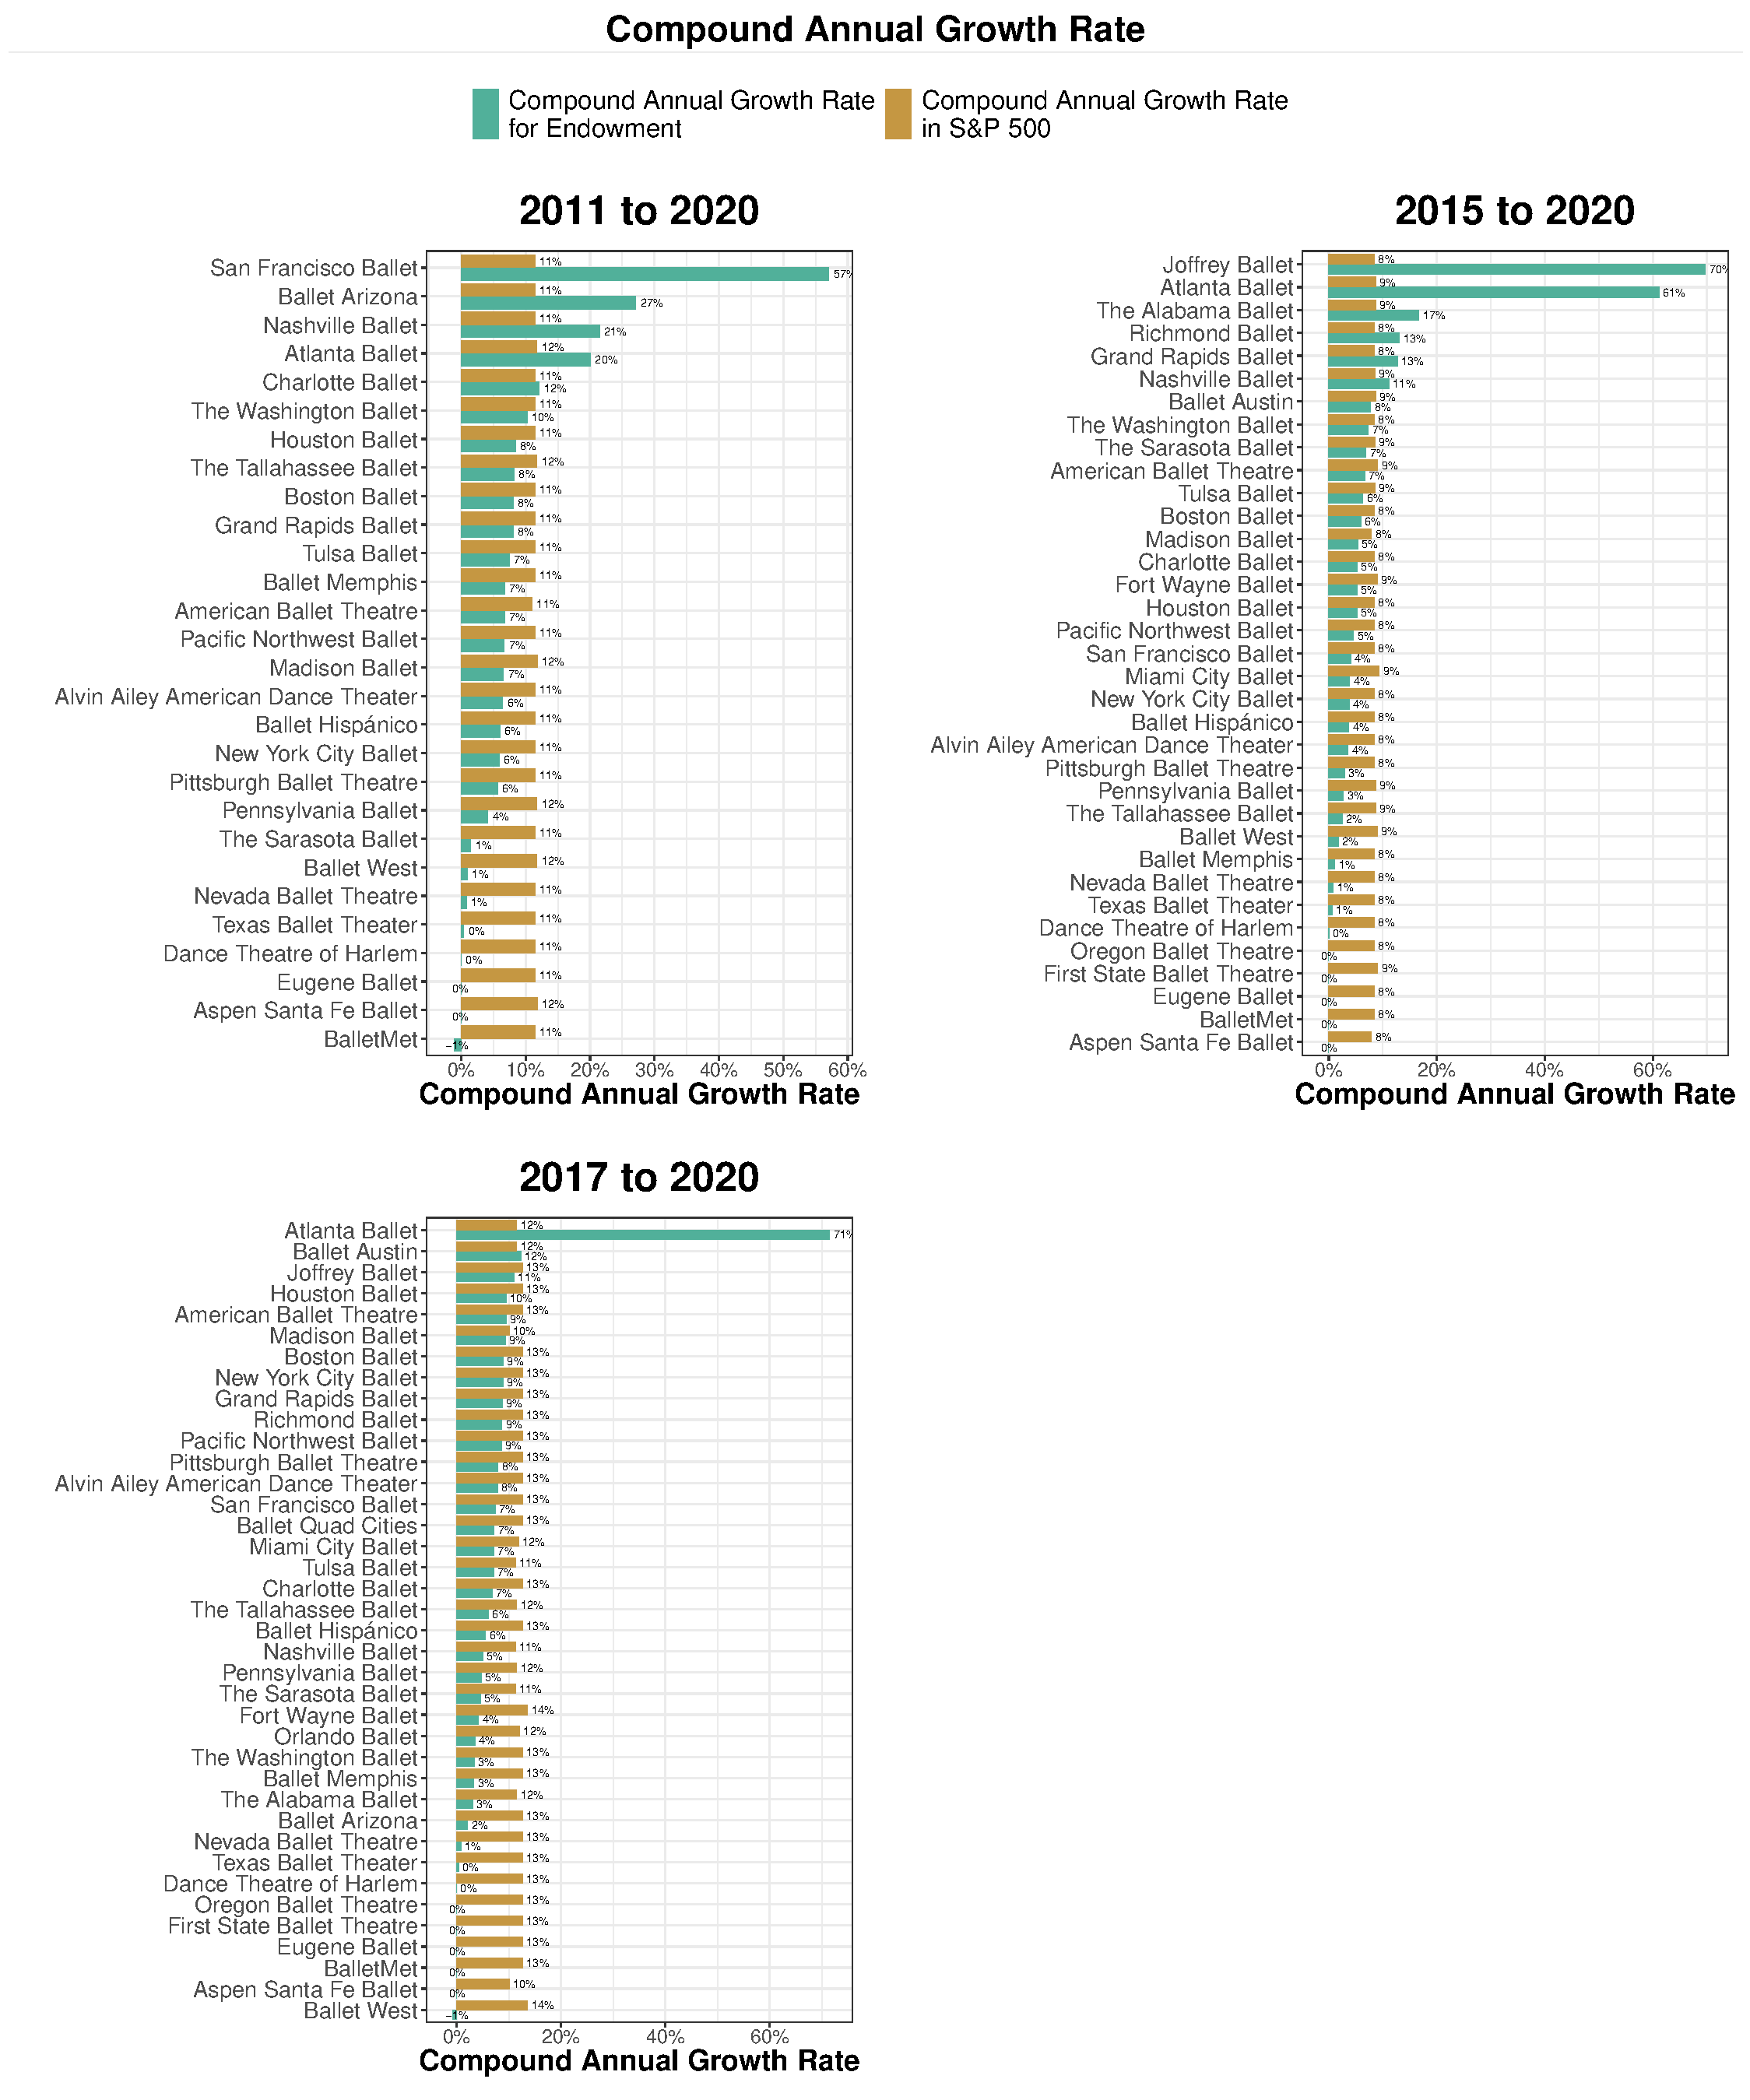
\includegraphics[width=0.9\linewidth,]{../images/compound-growth} \caption{\label{fig:compound-growth}Compound annual growth rates for all organizations compared to the compound annual growth rate for the S\&P 500 for three time periods. Not all companies are present in each plot, since not all companies have data going back the same number of years. Of note, year to year differences in the compound annual growth rate of the S\&P 500 are due to differences in companies' fiscal years.}\label{fig:unnamed-chunk-12}
\end{figure}

\begin{figure}[H]
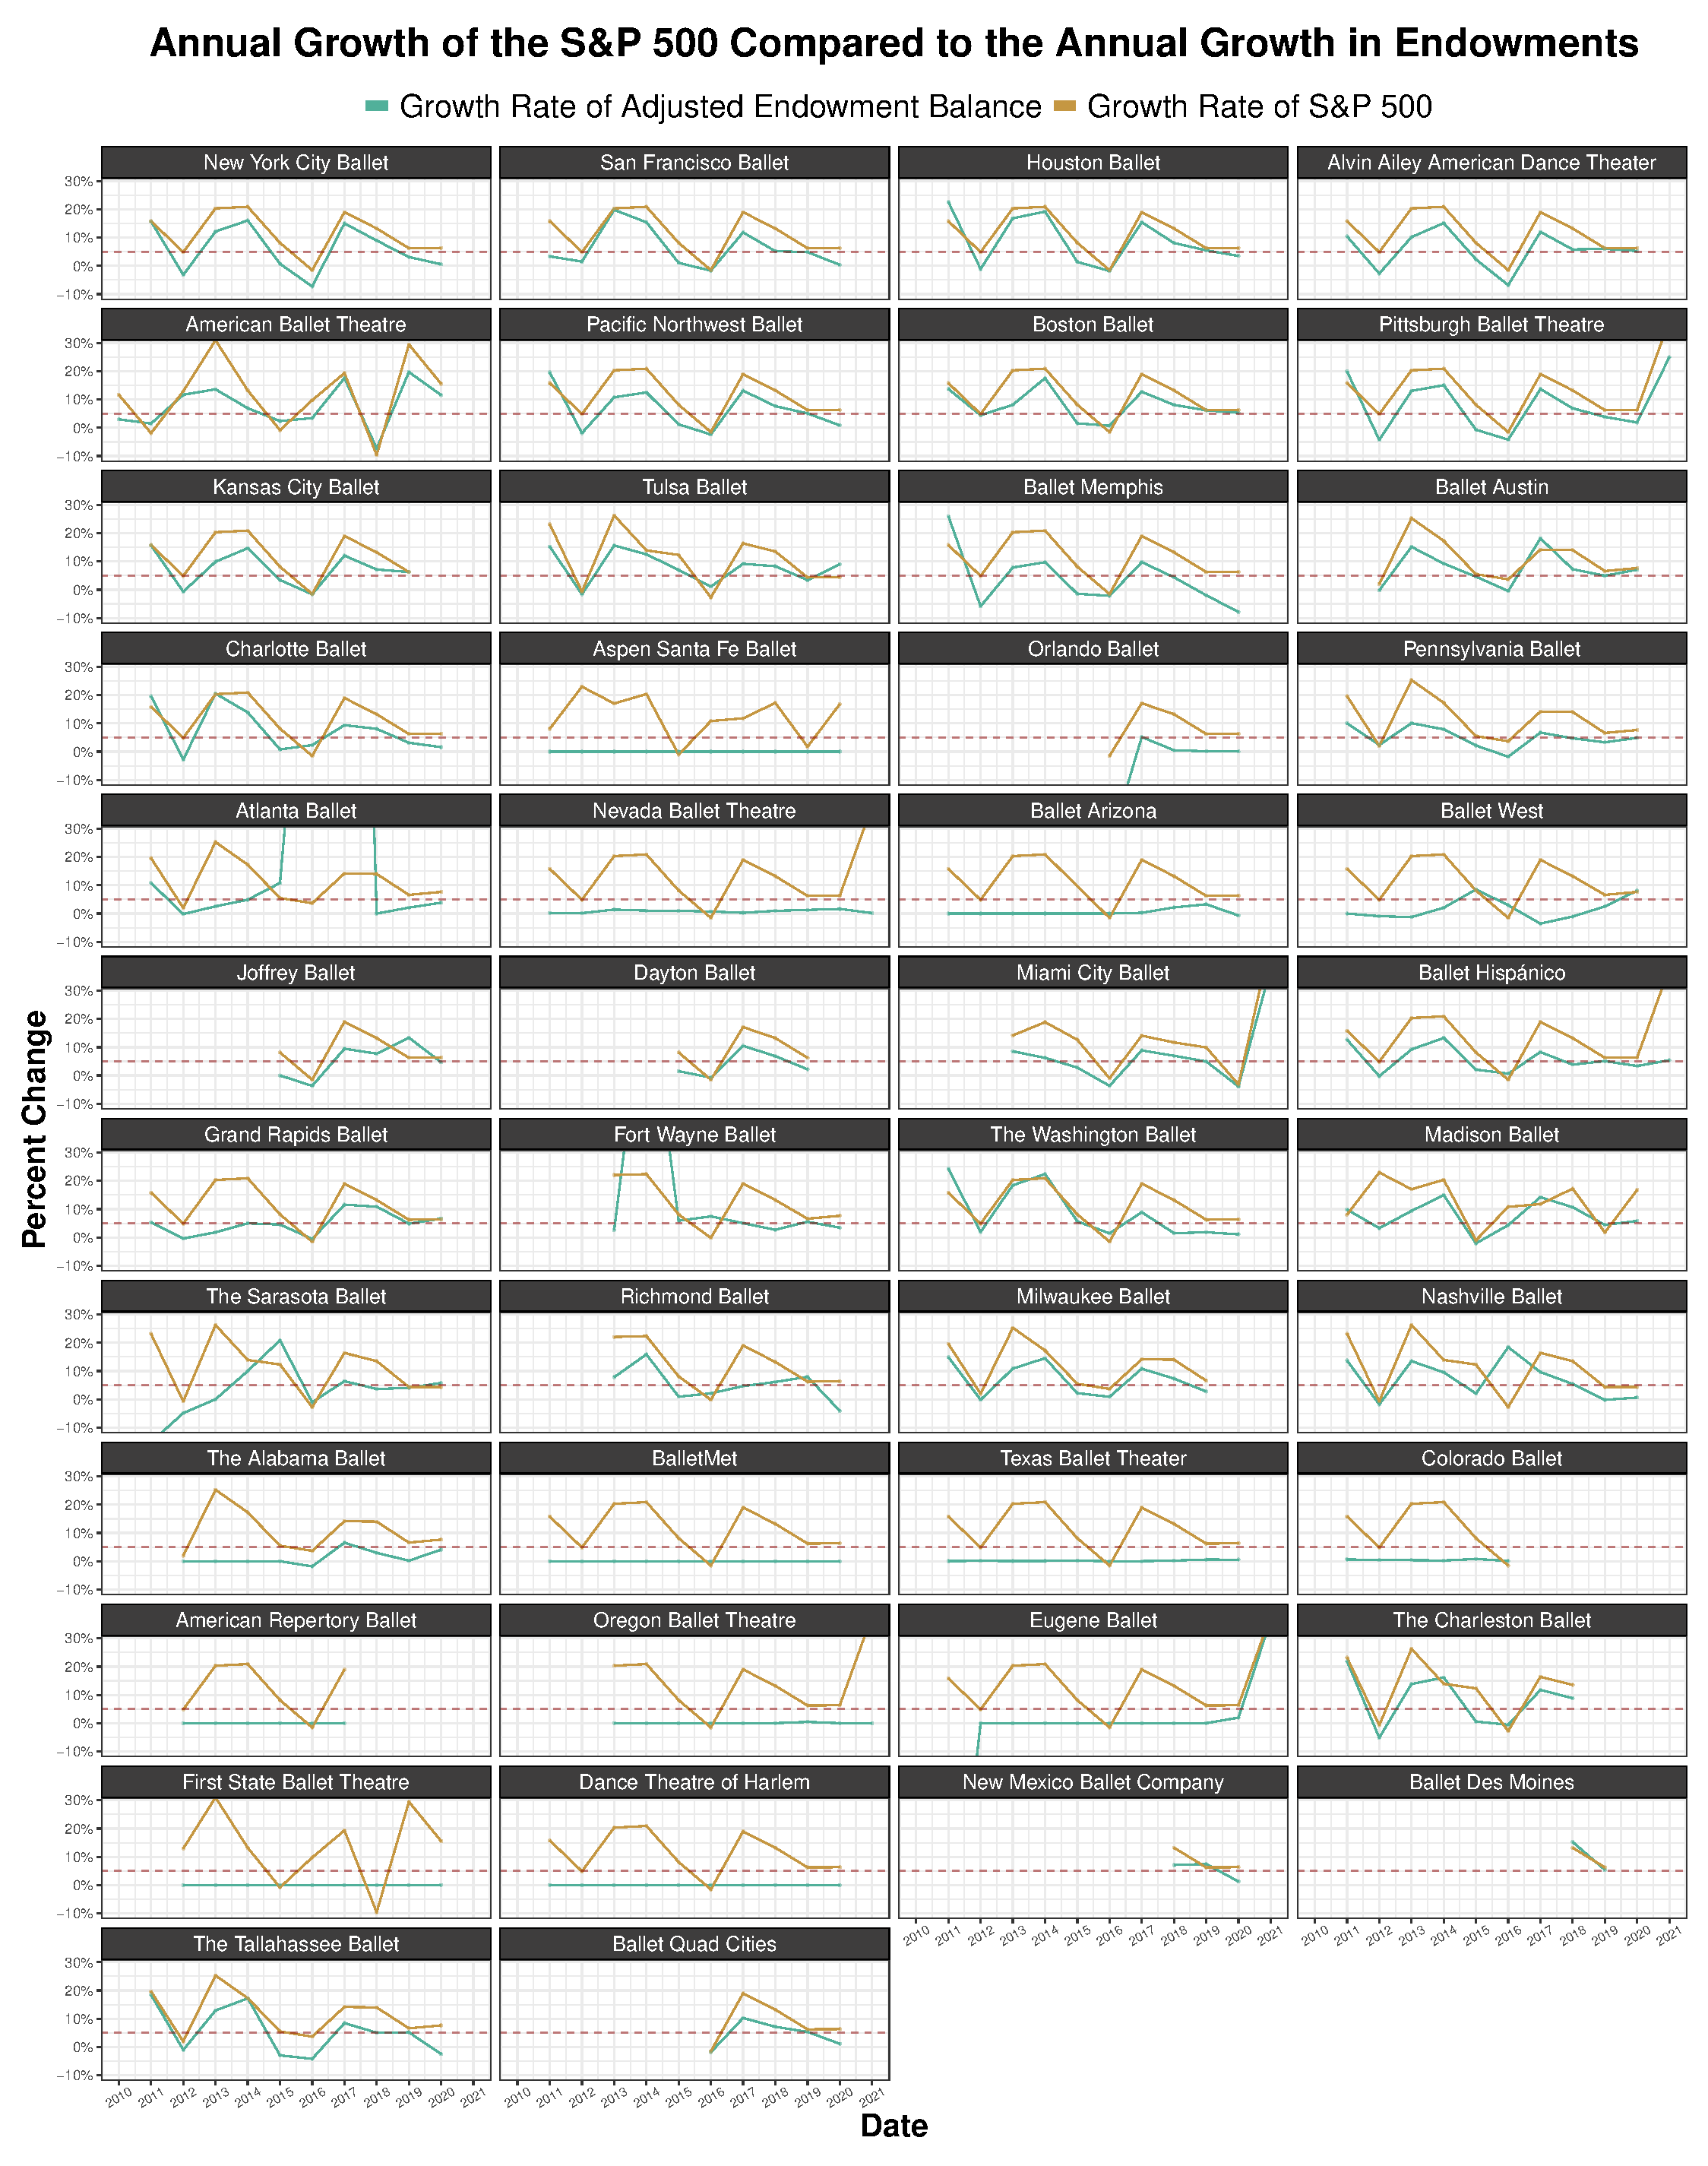
\includegraphics[width=0.9\linewidth,]{../images/annual-growth} \caption{\label{fig:annual-growth-endowment}Annual growth rate of a company's endowment when adjusting for contributions and withdrawals, compared to the annual growth S\&P 500 for the corresponding time period.}\label{fig:unnamed-chunk-13}
\end{figure}

\hypertarget{volunteer-paid-labor}{%
\subsection{Volunteer \& Paid Labor}\label{volunteer-paid-labor}}

\hypertarget{volunteer-labor-and-geography}{%
\subsubsection{Volunteer Labor and
Geography}\label{volunteer-labor-and-geography}}

As we see in Figure \ref{fig:type-region-bar}, the South has the most
companies who use more volunteers than employees with 68\% of all
reported companies volunteers, followed by the Midwest, then the West,
then Mid-America, New England, and finally the Mid-Atlantic.

\begin{figure}[H]
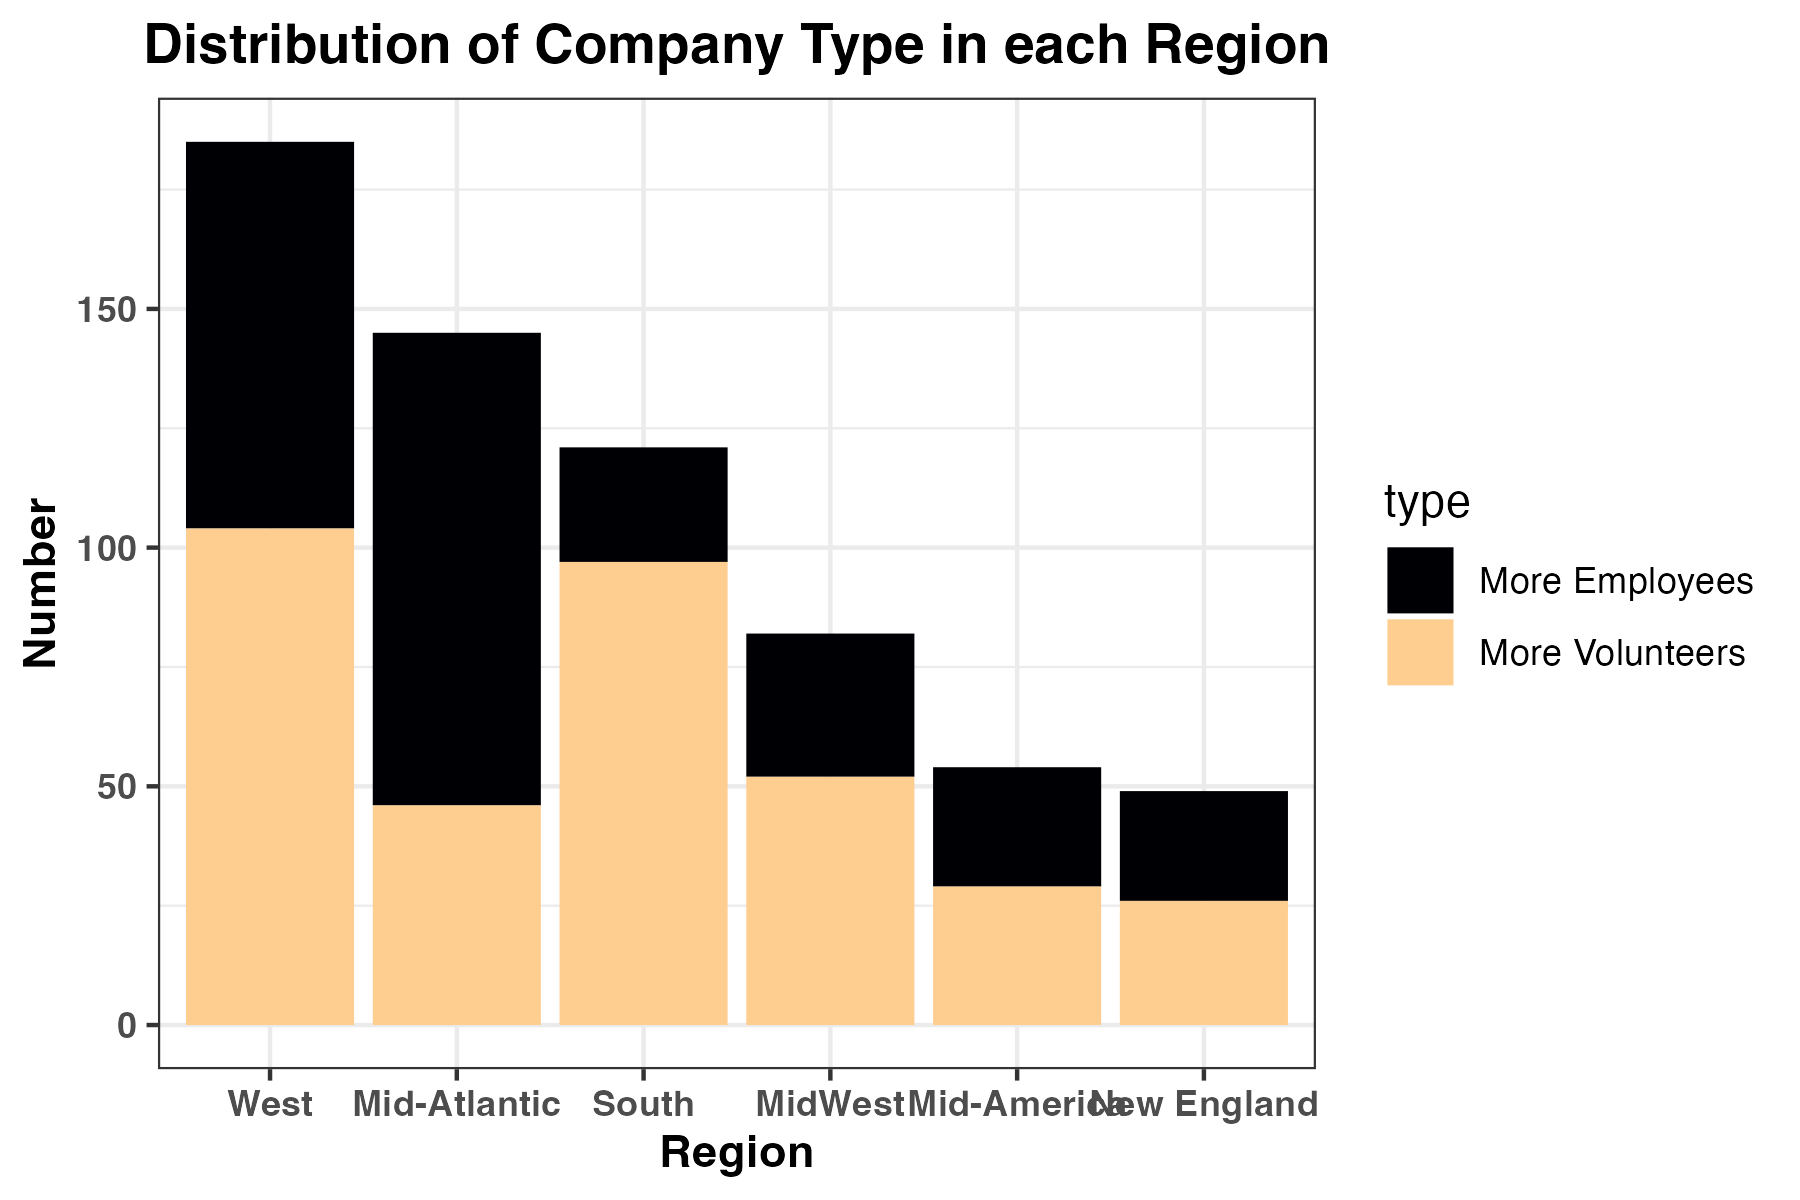
\includegraphics[width=0.9\linewidth,]{../images/type_region_bar} \caption{\label{fig:type-region-bar}Total number of laborers reported for each region in the 2019 fiscal year, colored by the number of companies who report either more employees or more volunteers}\label{fig:unnamed-chunk-14}
\end{figure}

In Figure \ref{fig:ratio-region}, we show the 1st, 2nd, 3rd, and 4th
quantiles of total volunteer labor. We ranked individual companies by
the total number of volunteers they reported and then computed the
quantiles. The share within each quantile is shown by region.

\begin{figure}[H]
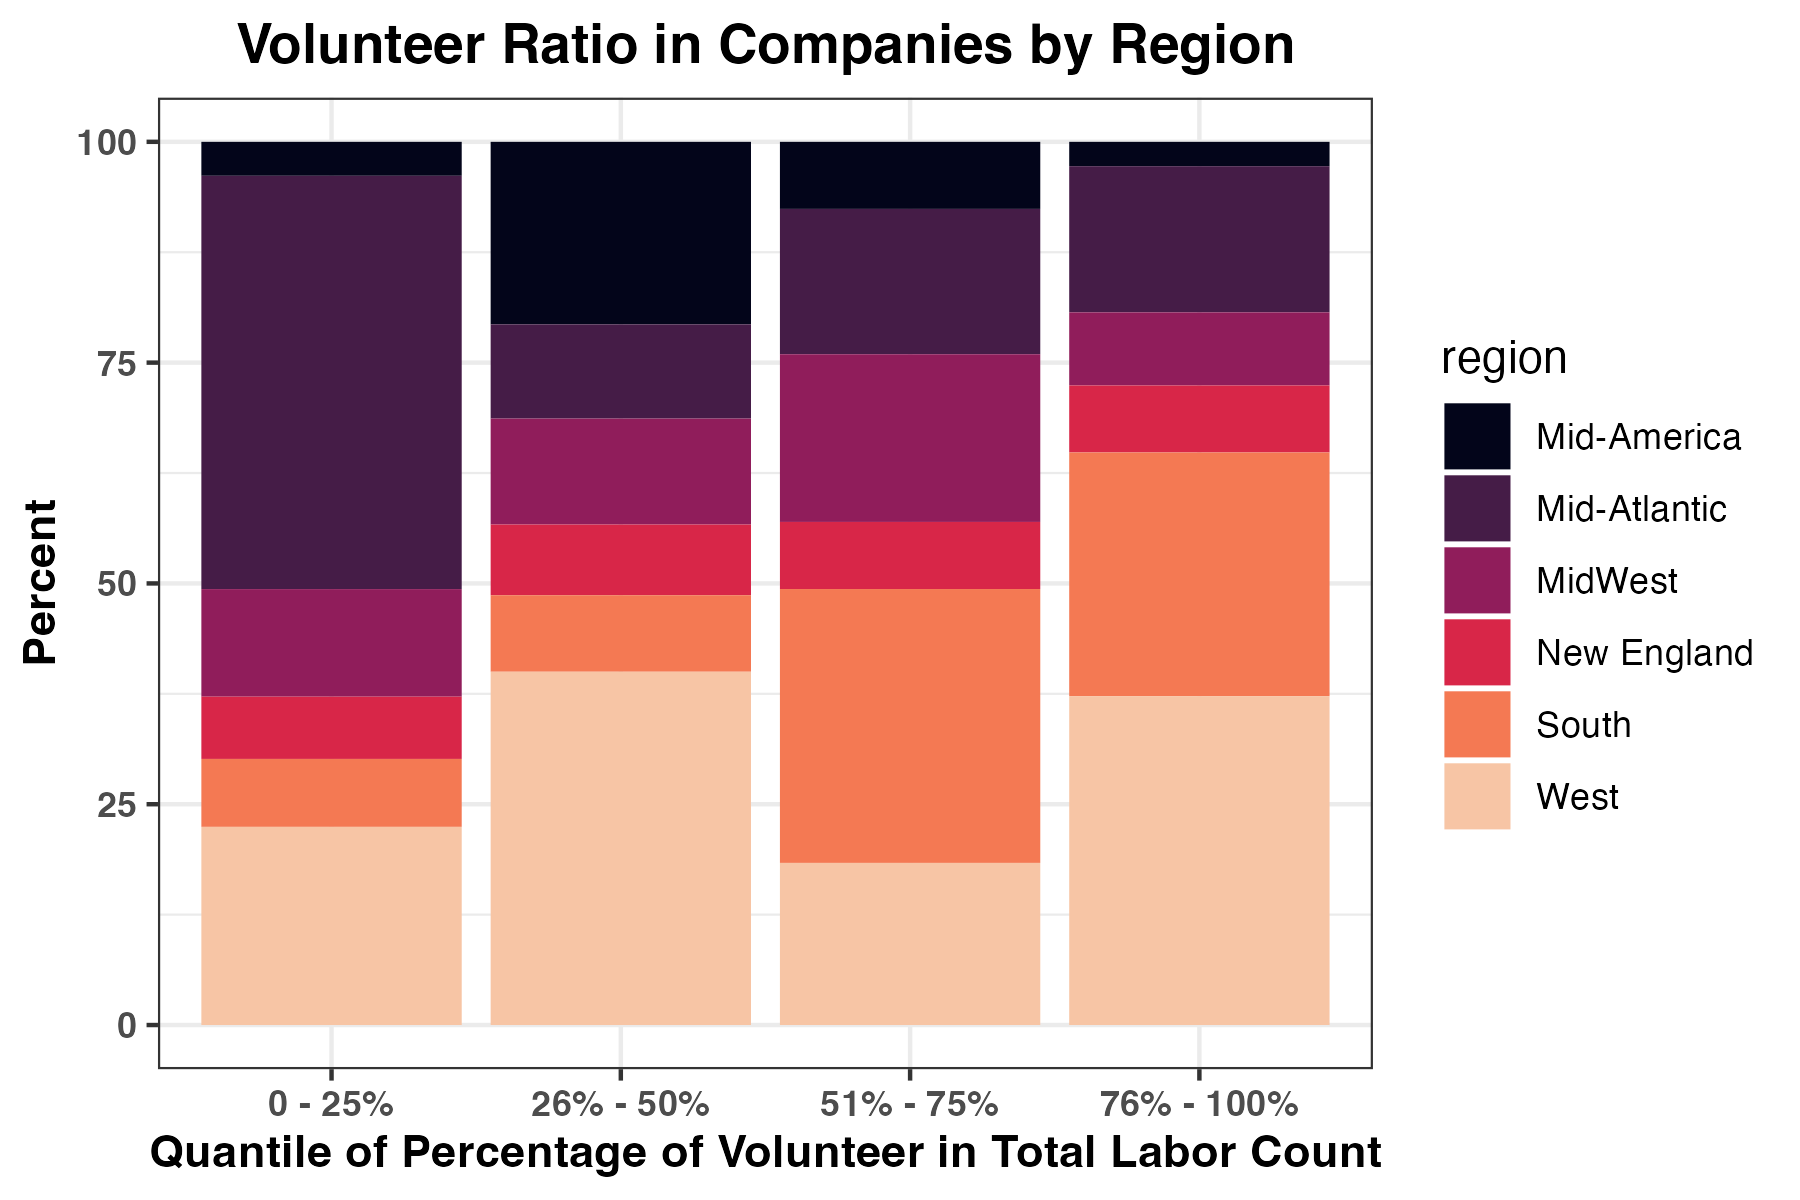
\includegraphics[width=0.9\linewidth,]{../images/ratio_bar_region} \caption{\label{fig:ratio-region}Share of volunteer use for each region by quantile using individual companies.}\label{fig:unnamed-chunk-15}
\end{figure}

We visualize the percentage of total labor that was volunteer labor by
state across the United States in Figure \ref{fig:us-map}.

\begin{figure}[H]
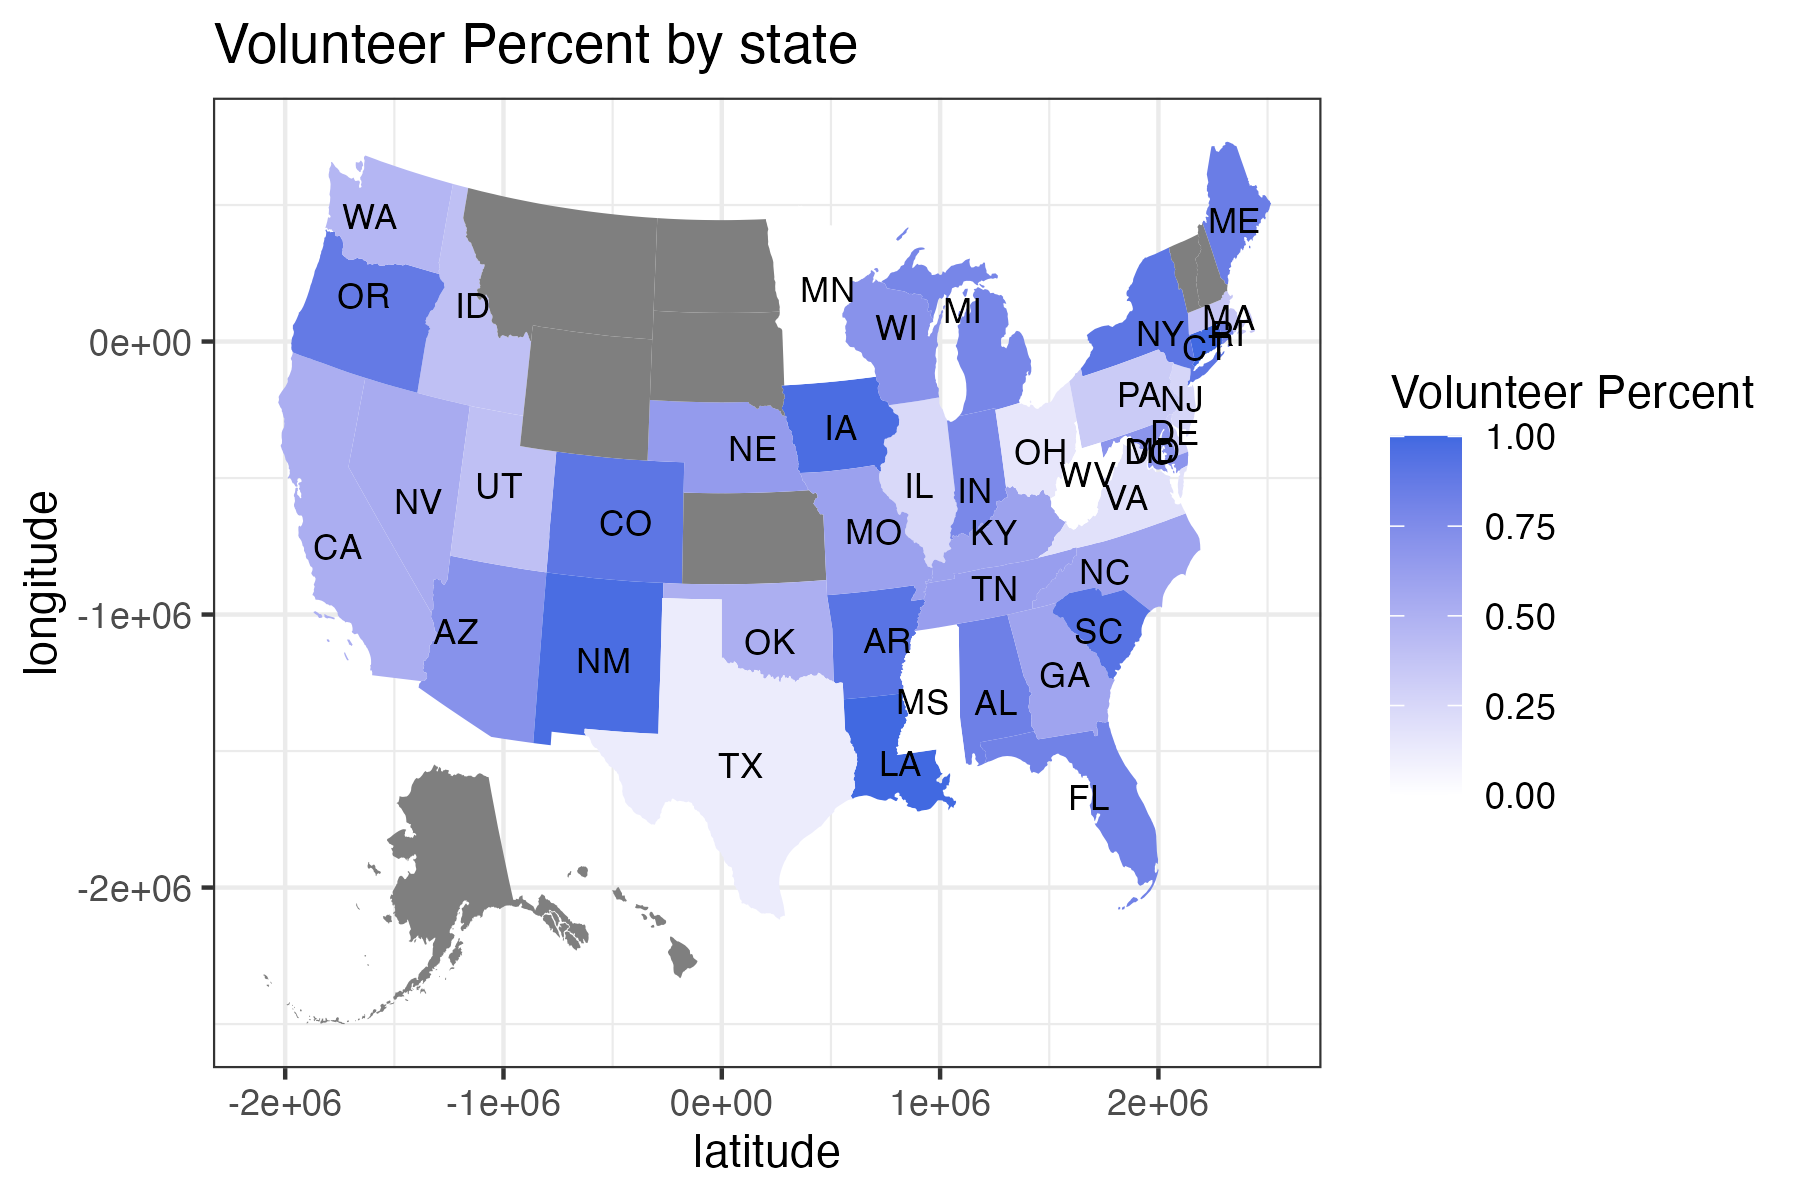
\includegraphics[width=0.9\linewidth,]{../images/vol_map} \caption{\label{fig:us-map}Share of volunteer labor among all labor by state. States, where we do not have data, are in gray.}\label{fig:unnamed-chunk-16}
\end{figure}

\hypertarget{compensation-totop-employees}{%
\subsubsection{Compensation toTop
Employees}\label{compensation-totop-employees}}

As we think about paid and unpaid labor in the dance industry, it is
also useful to look at how compensation is distributed among paid
employees.

In Part IX of the Form 990, companies report compensation going to the
set of top employees -- in particular, ``officers, directors, trustees,
and key employees''; we refer to this set of top employees as C-Suite
employees. Additionally, they report the total compensation to all
employees.

This information allows us to compare what percent of total employee
compensation was going to C-Suite employees. For this analysis, we only
included companies with more than 45 employees. This choice was due to
the extent of variability in the percentages paid to C-Suite employees
in companies smaller than this threshold size, since there are some
years where smaller companies report zero compensation to C-Suite
employees.

Of note, Aspen Santa Fe Ballet has previously contacted DDP ® regarding
C-Suite compensation, as they amended their fiscal year 2020 990s;
however, as the IRS is behind in its uploading of amended returns, we do
not have the corrected information.

The percentage paid to C-Suite employees ranges from 0\% to a little
over 30\%, and is fairly constant over the years (Figure
\ref{fig:frac-comp} ) . The median for each fiscal year was close to
10\%. However, we do see with the limited data available for 2021 that
percentages appear to increase following the onset of the pandemic; this
trend will be important to consider as more data from 2021 is released.

In Figure \ref{fig:csuite-comp-bar}, where we summarize the difference
in the percentage of total compensation paid to C-Suite employees in
2020 to that in 2015, we see there's actually fairly even split between
companies that increased the percent paid to C-Suite employees versus
those that decreased the percent going to C-Suite employees.

\begin{figure}[H]
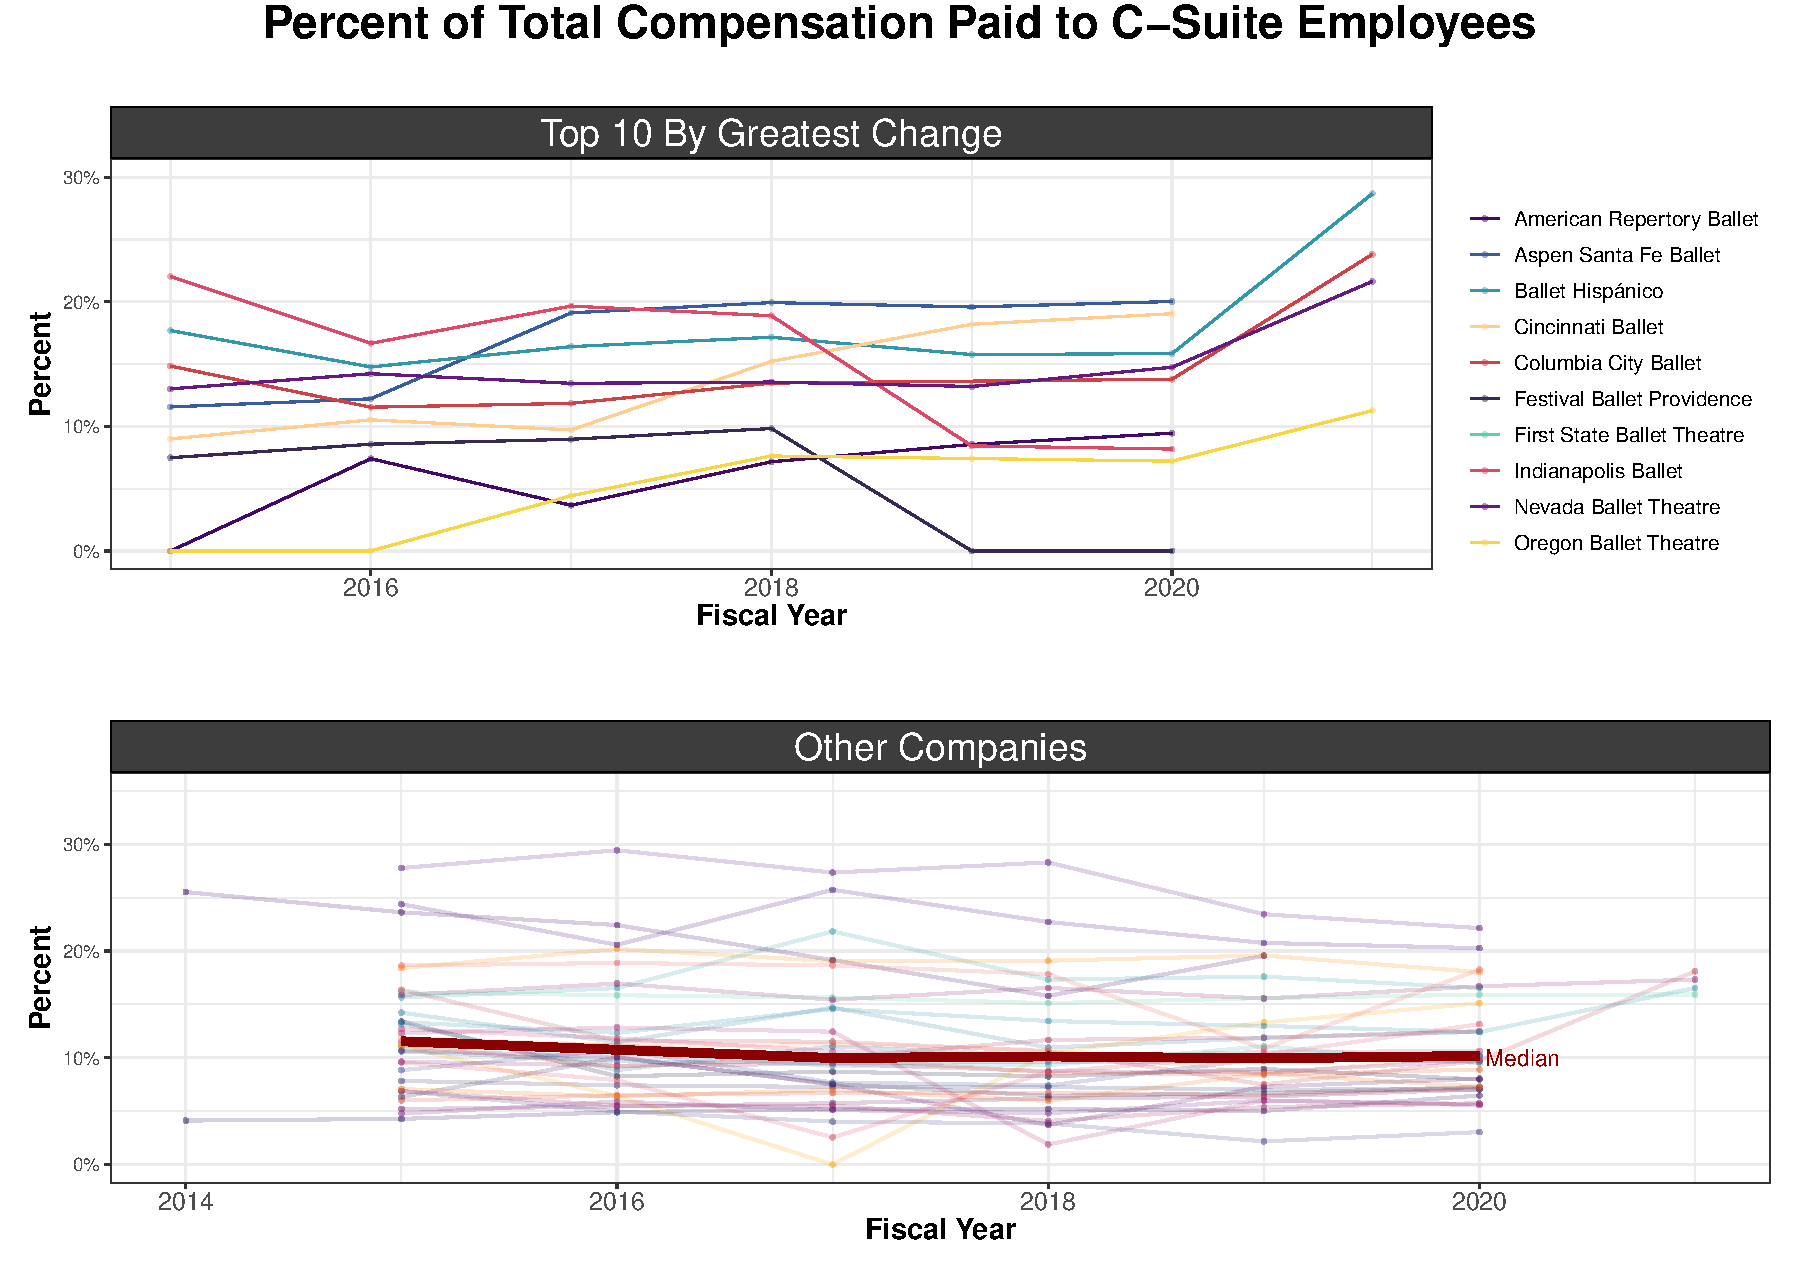
\includegraphics[width=0.9\linewidth,]{../images/frac-comp} \caption{\label{fig:frac-comp} percent of the total compensation paid to employees that was paid to officers, directors, trustees, or key employees, as reported in Part IX of the Form 990. Highlighted in the first panel are the 10 companies that had the greatest change in the percent paid to C-Suite employees from the earliest year on file to the latest. Only companies with more than 45 employees and that reported complete data for more than 5 years are included.}\label{fig:unnamed-chunk-17}
\end{figure}

\begin{figure}[H]
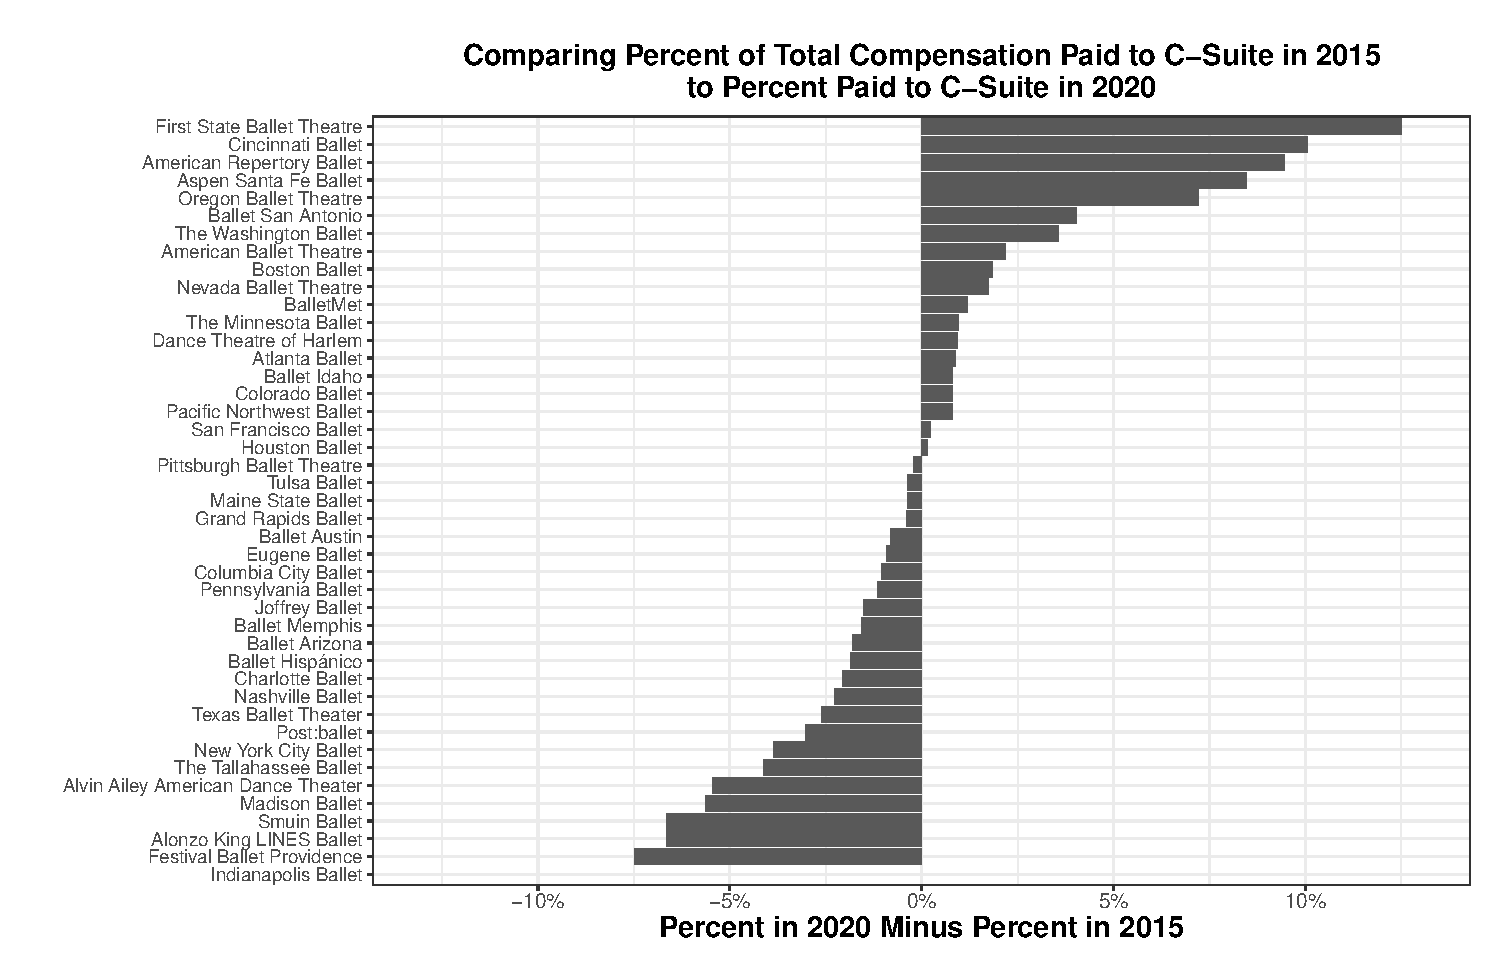
\includegraphics[width=0.9\linewidth,]{../images/csuite-comp-bar} \caption{\label{fig:csuite-comp-bar} Comparing the percent of total compensation paid to C-Suite employees in 2015 to that in 2020. Since we are subtracting the 2015 percent from the 2020 percent, positive values indicate a greater percent of compensation went to C-Suite employees in 2020, while negative values indicate a smaller percent of compensation went to C-Suite employees in 2020.}\label{fig:unnamed-chunk-18}
\end{figure}

\hypertarget{buildings}{%
\subsection{Buildings}\label{buildings}}

In-person performances are a huge part of dance companies' business, and
many of shows are held in companies' own theaters. Therefore, analyzing
how each company's endowment of buildings and lands, especially their
book values, is important in understanding how these companies are
faring economically. In this analysis, we define book values as the
value of the asset recorded on the balance sheet, as reported in Part VI
of Schedule D of the Form 990. For all the analyses included below, the
book values are summed from all the buildings and lands owned by the
company.

In the following plots, we consider one quantile at a time because these
values are on such different scales, with some companies approaching
\(8 \times 10^7\) in book values, while others had less than
\(1 \times 10^5\).

\hypertarget{the-trend-in-property-book-values-highmediumlow-by-quantile}{%
\subsubsection{The Trend in Property Book Values (high/medium/low by
quantile)}\label{the-trend-in-property-book-values-highmediumlow-by-quantile}}

\begin{figure}[H]
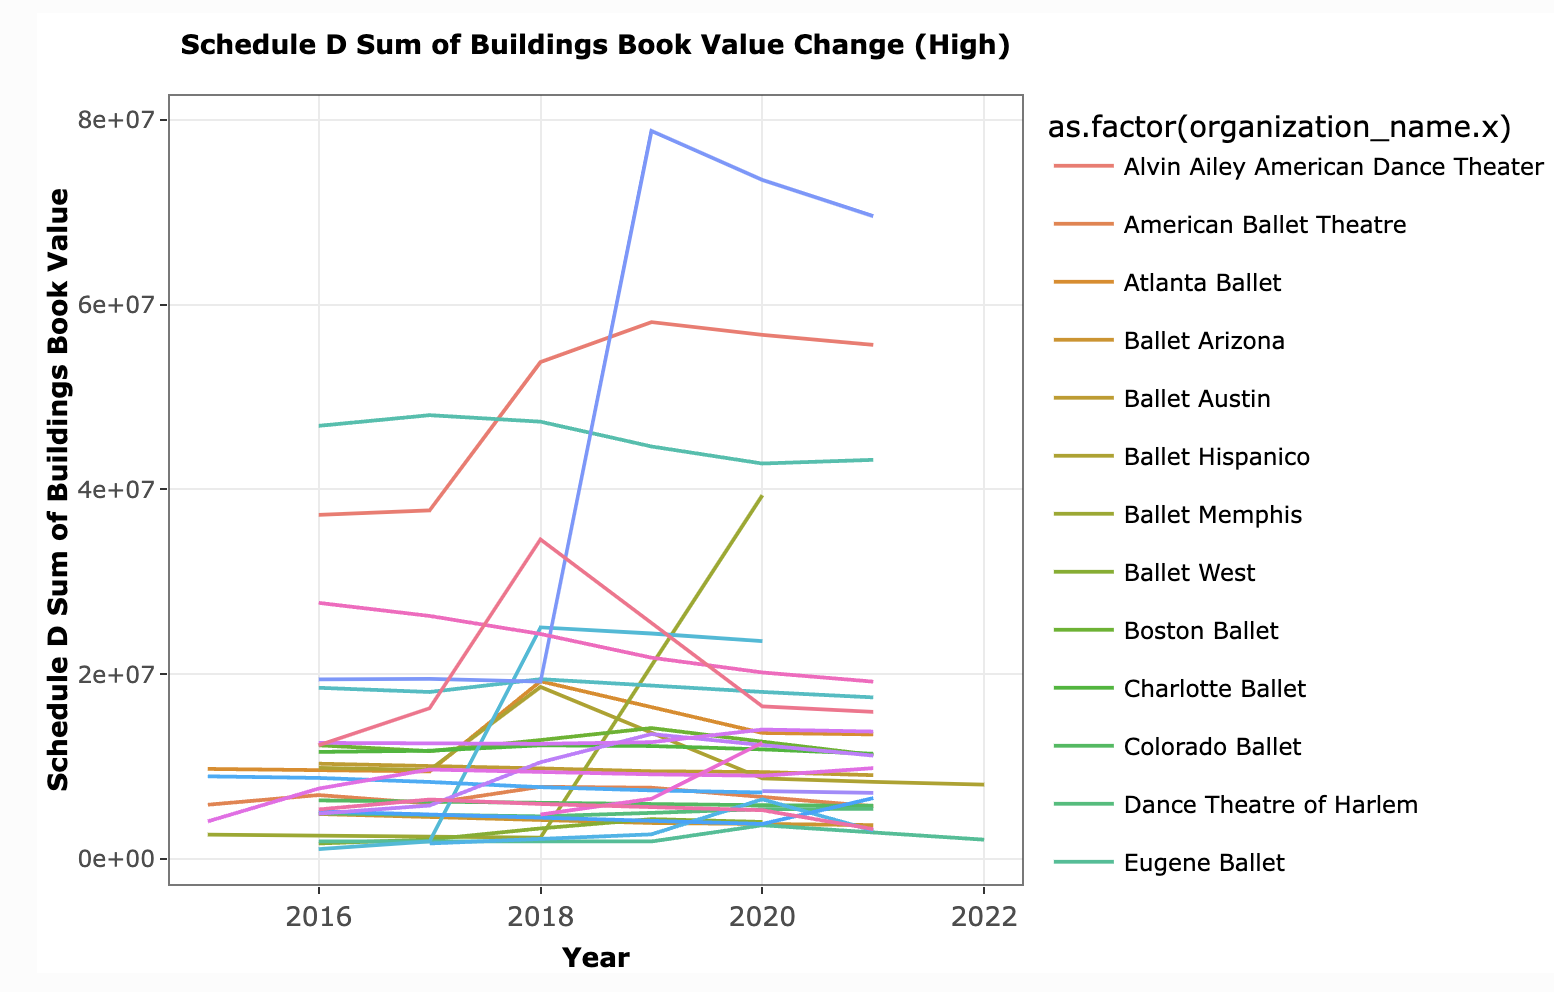
\includegraphics[width=0.8\linewidth,]{../images/high} \caption{\label{fig:high}}\label{fig:unnamed-chunk-19}
\end{figure}

\begin{figure}[H]
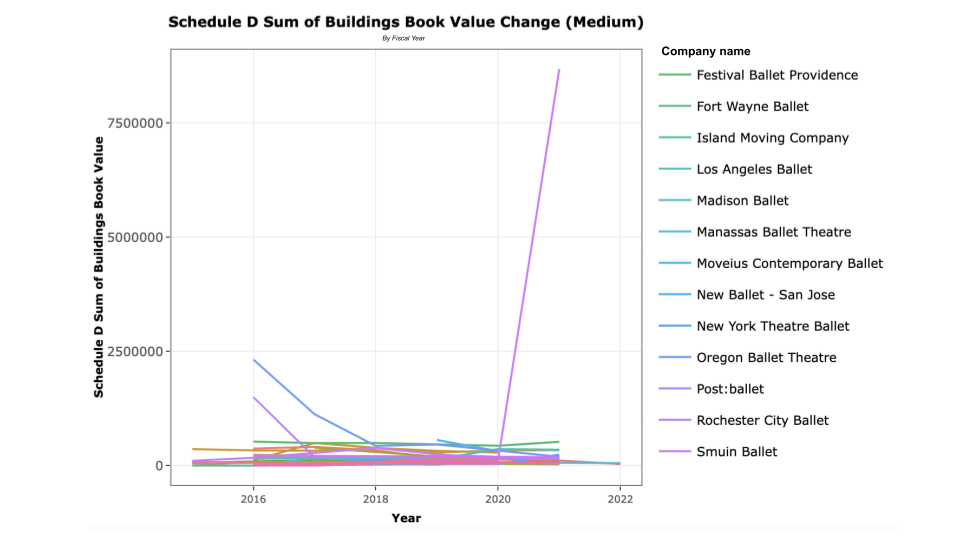
\includegraphics[width=0.8\linewidth,]{../images/medium} \caption{\label{fig:medium}}\label{fig:unnamed-chunk-20}
\end{figure}

\begin{figure}[H]
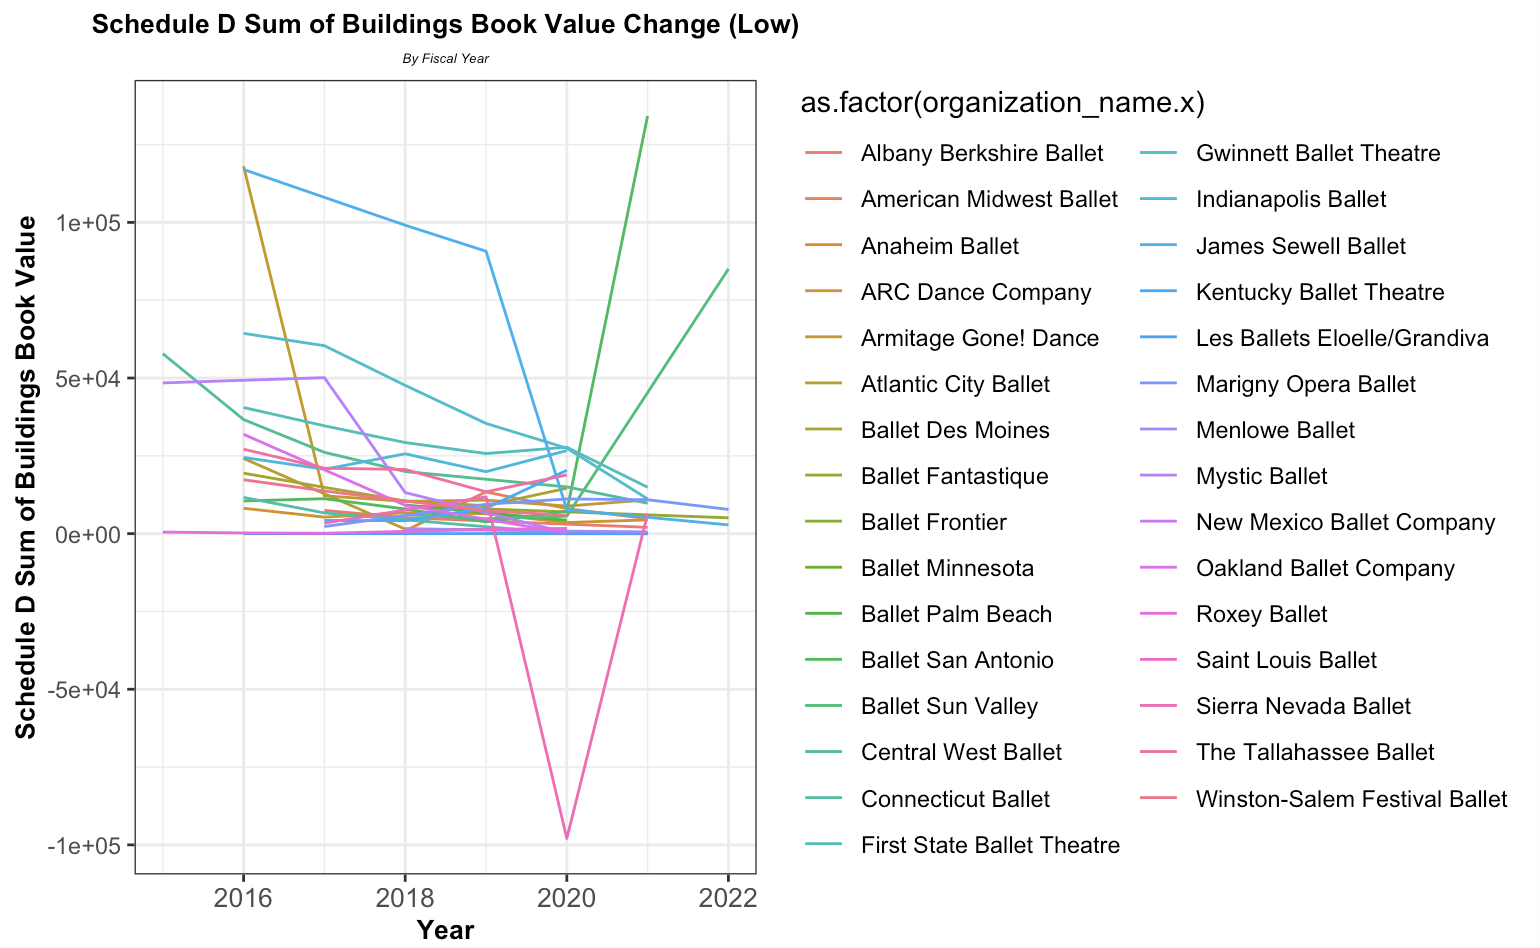
\includegraphics[width=0.8\linewidth,]{../images/low} \caption{\label{fig:low}}\label{fig:unnamed-chunk-21}
\end{figure}

In Figures \ref{fig:high}, \ref{fig:medium}, and \ref{fig:low}, we see
the percent changes in buildings' book values for each company from 2014
to 2021. We divided companies into three groups based on their
building's book value: high, medium, and low, based on the quantile of
their book values in 2020. Companies with notable changes for each
category are:

\begin{itemize}
\tightlist
\item
  Major: New York City Ballet, Ballet Memphis, Tulsa Ballet.\\
\item
  Medium: Smuin Ballet\\
\item
  Low: Saint Louis Ballet, Les Ballets Eloelle/Grandiva, Ballet Palm
  Beach, Ballet
\end{itemize}

\hypertarget{percent-change-in-building-book-values}{%
\subsubsection{Percent change in Building Book
Values}\label{percent-change-in-building-book-values}}

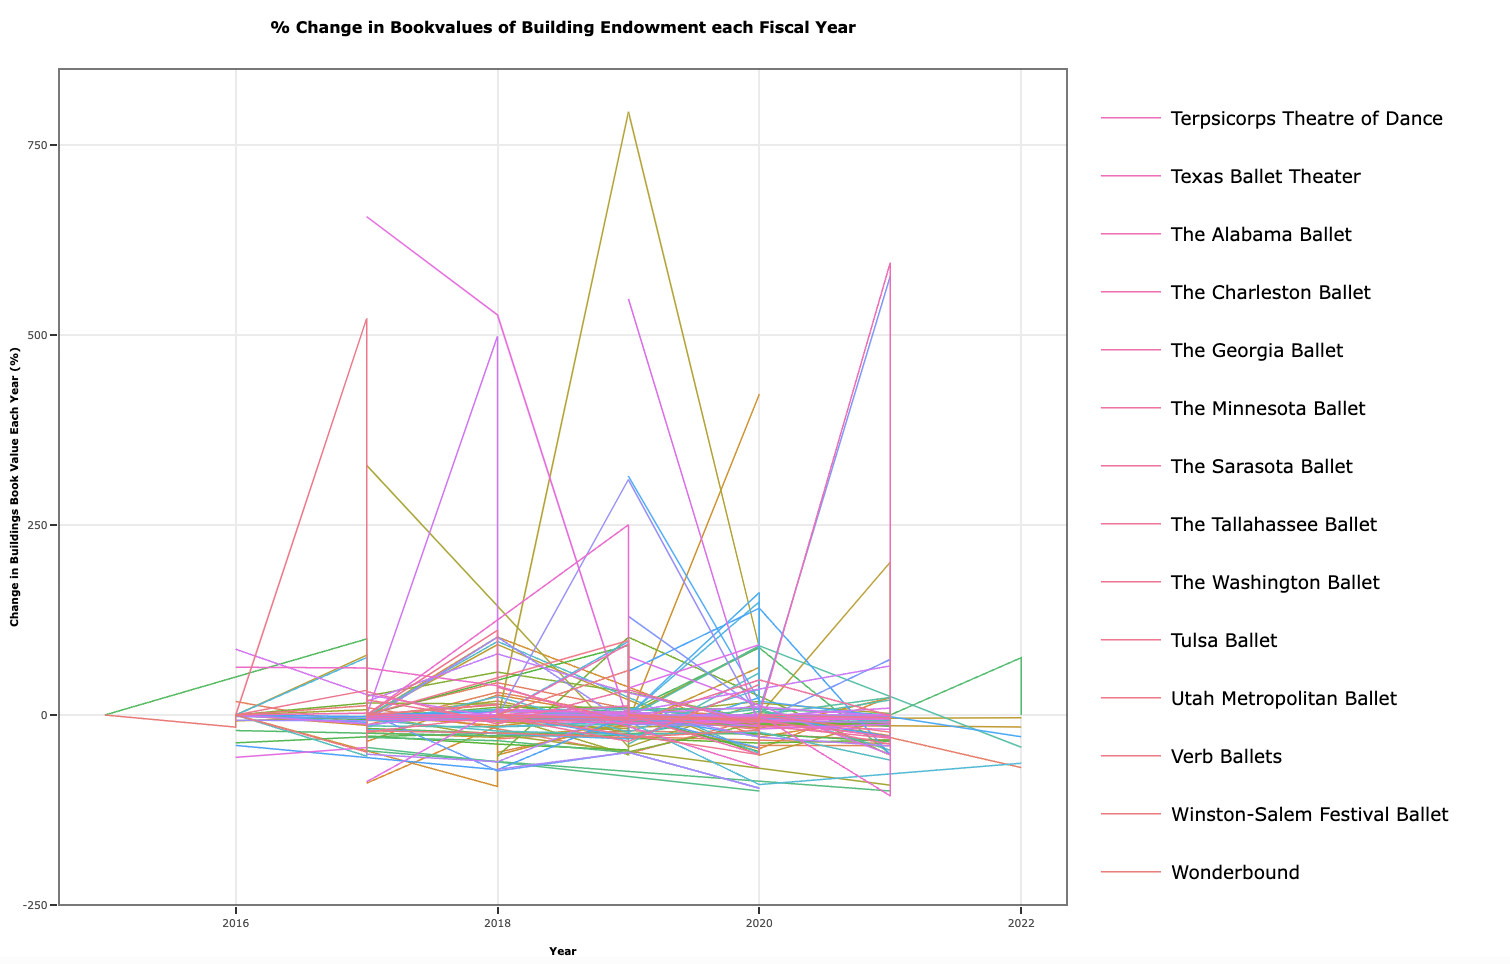
\includegraphics[width=0.9\linewidth,]{../images/percentage_building}

Most companies did not go through large changes in book values of
buildings in their endowment besides depreciation. The companies went
through larger changes include Utah Metropolitan Ballet, Post:ballet,
Ballet Memphis, Philadanco, New Ballet San Jose, Sacramento Ballet,
Marigny Opera Ballet, and Ballet Idaho.

\hypertarget{percent-change-in-ranking}{%
\subsubsection{Percent Change in
Ranking}\label{percent-change-in-ranking}}

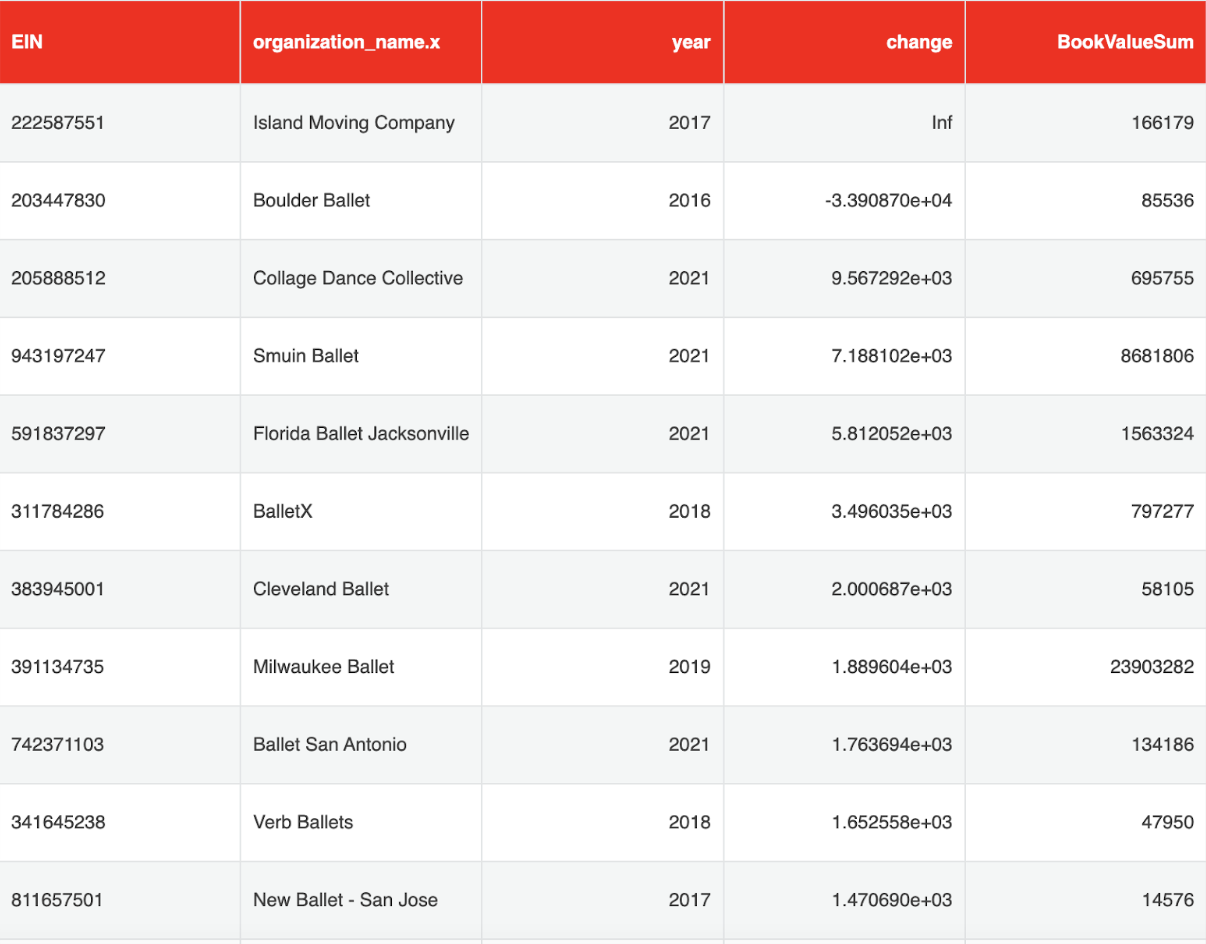
\includegraphics[width=0.6\linewidth,]{../images/percent_change_ranking}

\hypertarget{percentage-change-in-book-value-by-year}{%
\subsubsection{Percentage change in book value by
year}\label{percentage-change-in-book-value-by-year}}

We can see from the mean that many extreme values exist in terms of
changes in the building's book values.

\hypertarget{conclusions}{%
\section{Conclusions}\label{conclusions}}

\hypertarget{data-quality}{%
\subsection{Data Quality}\label{data-quality}}

As stated in the introduction, online reporting of tax returns by dance
companies has facilitated this research; however, a long-standing issue
with publicly-available tax reporting is there is no guarantee that
mistakes are not made and published. Therefore, a significant part of
our analyses were focused on checking the quality, completeness, and
aberrations in values reported on the 990 forms. We found many
discrepancies indicating non-concordance concerning the end of year
balances and beginning year balances within the same year for many
companies, where the values reported don't match indicating missing
information. Additionally, values reported for previous years did not
match what certain companies actually filed for those years with no
apparent explanation. Many companies we reached out to for clarification
did not respond. This issue should be addressed in future analyses.
Implications for missing or inaccurate reporting on form 990s and 990EZs
include misinforming the public. Data analyses run on inaccurate
information may also draw false conclusions towards financial practices
of certain companies that don't really exist. Informing dance companies
on the importance of proper tax reporting may help address these errors
in the future.

\hypertarget{endowments-and-the-sp-500}{%
\subsection{Endowments and the S\&P
500}\label{endowments-and-the-sp-500}}

Our analyses have demonstrated that the trends of the stock market, and
particularly the S\&P 500, heavily influence percent change in the
endowments of many companies. Other companies perform very differently
from the S\&P 500. This indicates that companies significantly differ in
their investment behavior. Some companies differ in their investment
behavior. Some companies, such as Oregon Ballet Theatre and Aspen Santa
Fe Ballet, did not invest their endowments at all. Others, including San
Fransico Ballet, Arizona Ballet, Joffrey Ballet, and Houston Ballet, saw
substantial investment gains over the years we analyzed. This has
significant implications for the individual dancers employed by these
companies in terms of compensation opportunities as well as job
security. A company that does not earn investment income risks long-term
operation deficits due to inflation and unforeseen expenses. Therefore,
it is important to continue to examine changes in endowments for dance
companies over time and clearly communicate these findings to the dance
world.

\hypertarget{employee-and-volunteer-labor}{%
\subsection{Employee and Volunteer
Labor}\label{employee-and-volunteer-labor}}

\hypertarget{by-geographical-region}{%
\subsubsection{By Geographical Region}\label{by-geographical-region}}

Overall, more labor (both volunteer and employee) is used in the West,
followed by the Mid-Atlantic, then the South, then the Midwest, then
Mid-America, and finally New England. Of these regions, the one with the
highest proportion of companies who rely more on volunteer labor than
paid employees is the Midwest, followed by the West, then Mid-America,
New England, and then the Mid-Atlantic. This indicates that a few things
could be happening in the world of dance. First, in regions with high
rates of volunteer labor, there may be a higher percentage of community
engagement. This is especially true for companies such as Eugene Dance
in Oregon from the West region, which reports a significant number of
volunteers but generates significant community support for their
productions. Secondly, in regions with high rates of employee labor,
state, and local governments may subsidize compensation costs which
increase companies' ability to hire and pay their employees. Since dance
is known to be an industry with a disproportionate amount of unpaid
labor, it is especially important to understand where and why these
discrepancies occur.

\hypertarget{compensation-and-building-value}{%
\subsection{Compensation and Building
Value}\label{compensation-and-building-value}}

We also examined the fraction of compensation going to senior executives
(i.e.~their C-Suite employees) is generally consistent. Future research
should track trends of executive compensation throughout the pandemic.
Additionally, the pattern of how dance companies use their building
endowment is inconsistent. Further investigation is required to fully
understand why and how real estate is used by these companies.

The wide-ranging impacts of these understandings may lead to greater
awareness by unpaid and underpaid laborers in dance, accountability for
dance companies, and more equity in the dance industry. We hope this
work provides motivation for further investigation of dance companies'
publicly available 990 data to better understand the financial
performance and decisions of dance companies, as well as other companies
in the performing arts.

\hypertarget{limitations}{%
\section{Limitations}\label{limitations}}

Our analyses were not without limitations. First, certain companies have
discrepancies in their End-of-Year and Beginning-of-Year balances. We
used End-of-Year balances to calculate the percent change in endowments
of all dance companies, so some information may be misrepresented based
on these discrepancies. Additionally, data on a finer time scale, for
example at the monthly time scale rather than the yearly, would be more
informative for studying how investments did over time; however, 990
Forms only provide this data annually. Another limitation of this work
is the analysis of compensation. The Form 990 provides summarized
information across total employees, along with some information about
compensation to C-Suite executives. However, we cannot tell directly
from this data which of these employees are dancers, and as such, we
cannot tell how dancers are being compensated relative to other
employees. Finally, a significant number of companies did not report
their number of employees and/or their number of volunteers. This led to
missing data that was left out the geographical and unpaid labor
analyses. Nine states (New Hampshire, Vermont, Kansas, Wyoming, South
Dakota, North Dakota, Montana, Hawaii, and Alaska) did not have any
companies in this analysis.

\hypertarget{future-research}{%
\section{Future Research}\label{future-research}}

Because the IRS is greatly behind on releasing Form 990s, we only have
data from 2021 for a smaller subset of companies, 29 companies in total.
That said, the effect of the COVID-19 pandemic on all trends we have
examined here is a crucial area of future research. Because the federal
government issued billions of dollars in public subsidies, trends
throughout the pandemic would be helpful to identify whether these
subsidies helped those intended. Similarly, we would like to see if the
COVID-19 pandemic has changed the way companies used and reported their
building endowment found in this study, Lockdown policies in each state
might change how in-person performances were held, and companies might
shut down certain performance centers due to prolonged quarantine.
Therefore, future research on buildings' book values should be conducted
after more data in 2021 and 2022 is uploaded. Yet, to date, no
comprehensive analysis has been done on the wage gap in dance throughout
the pandemic. Once tax documents through 2022 are filed for these
companies, future research can examine how wages, income, operations,
and unpaid labor at dance companies have evolved throughout the
pandemic.

% %%%%%%%%%%%%%%%%%%%%%%%%%%%%%%%%%%%%%%%%%%
% %% optional
% \supplementary{The following are available online at www.mdpi.com/link, Figure S1: title, Table S1: title, Video S1: title.}
%
% % Only for the journal Methods and Protocols:
% % If you wish to submit a video article, please do so with any other supplementary material.
% % \supplementary{The following are available at www.mdpi.com/link: Figure S1: title, Table S1: title, Video S1: title. A supporting video article is available at doi: link.}

\vspace{6pt}

%%%%%%%%%%%%%%%%%%%%%%%%%%%%%%%%%%%%%%%%%%
\acknowledgments{The authors thank the support and mentorship of
Dr.~Lindsay Poirier, Andrew Hoekstra, and Elizabeth Yntema.}

%%%%%%%%%%%%%%%%%%%%%%%%%%%%%%%%%%%%%%%%%%

%%%%%%%%%%%%%%%%%%%%%%%%%%%%%%%%%%%%%%%%%%
\conflictsofinterest{The authors declare no conflict of interest.}

%%%%%%%%%%%%%%%%%%%%%%%%%%%%%%%%%%%%%%%%%%
%% optional
\abbreviations{The following abbreviations are used in this manuscript:\\

\noindent
\begin{tabular}{@{}ll}
DDP ® & Dance Data Project ® \\
IRS & Internal Revenue Service \\
\end{tabular}}


%%%%%%%%%%%%%%%%%%%%%%%%%%%%%%%%%%%%%%%%%%
% Citations and References in Supplementary files are permitted provided that they also appear in the reference list here.

%=====================================
% References, variant A: internal bibliography
%=====================================
%\reftitle{References}
%\begin{thebibliography}{999}
% Reference 1
%\bibitem[Author1(year)]{ref-journal}
%Author1, T. The title of the cited article. {\em Journal Abbreviation} {\bf 2008}, {\em 10}, 142--149.
% Reference 2
%\bibitem[Author2(year)]{ref-book}
%Author2, L. The title of the cited contribution. In {\em The Book Title}; Editor1, F., Editor2, A., Eds.; Publishing House: City, Country, 2007; pp. 32--58.
%\end{thebibliography}

% The following MDPI journals use author-date citation: Arts, Econometrics, Economies, Genealogy, Humanities, IJFS, JRFM, Laws, Religions, Risks, Social Sciences. For those journals, please follow the formatting guidelines on http://www.mdpi.com/authors/references
% To cite two works by the same author: \citeauthor{ref-journal-1a} (\citeyear{ref-journal-1a}, \citeyear{ref-journal-1b}). This produces: Whittaker (1967, 1975)
% To cite two works by the same author with specific pages: \citeauthor{ref-journal-3a} (\citeyear{ref-journal-3a}, p. 328; \citeyear{ref-journal-3b}, p.475). This produces: Wong (1999, p. 328; 2000, p. 475)

%=====================================
% References, variant B: external bibliography
%=====================================
\reftitle{References}
\externalbibliography{yes}
\bibliography{DDPCitations.bib}

%%%%%%%%%%%%%%%%%%%%%%%%%%%%%%%%%%%%%%%%%%
%% optional

%% for journal Sci
%\reviewreports{\\
%Reviewer 1 comments and authors’ response\\
%Reviewer 2 comments and authors’ response\\
%Reviewer 3 comments and authors’ response
%}

%%%%%%%%%%%%%%%%%%%%%%%%%%%%%%%%%%%%%%%%%%


\end{document}
